% Targeted for International Journal of Medical Informatics
% Word limit: 3000
%\documentclass[review]{elsarticle}
\documentclass{elsarticle}


\usepackage{lineno,hyperref,graphicx}
\usepackage{amsmath}
\usepackage{amsfonts}
\usepackage[table]{xcolor}
\usepackage[section]{placeins}
\modulolinenumbers[5]
\graphicspath{ {./images/} }

% Adapted from https://www.overleaf.com/learn/how-to/Is_there_a_way_to_run_a_word_count_that_doesn%27t_include_LaTeX_commands%3F
\newcommand{\wordcount}[2]{%
  (\immediate\write18{texcount -1 -sum -merge #1.tex > #1-words.sum }%
  \input{#1-words.sum}/#2 words)%
}

\journal{Elsevier}

%%%%%%%%%%%%%%%%%%%%%%%
%% Elsevier bibliography styles
%%%%%%%%%%%%%%%%%%%%%%%
%% To change the style, put a % in front of the second line of the current style and
%% remove the % from the second line of the style you would like to use.
%%%%%%%%%%%%%%%%%%%%%%%

%% Numbered
%\bibliographystyle{model1-num-names}

%% Numbered without titles
%\bibliographystyle{model1a-num-names}

%% Harvard
%\bibliographystyle{model2-names.bst}\biboptions{authoryear}

%% Vancouver numbered
%\usepackage{numcompress}\bibliographystyle{model3-num-names}

%% Vancouver name/year
%\usepackage{numcompress}\bibliographystyle{model4-names}\biboptions{authoryear}

%% APA style
%\bibliographystyle{model5-names}\biboptions{authoryear}

%% AMA style
%\usepackage{numcompress}\bibliographystyle{model6-num-names}

%% `Elsevier LaTeX' style
\bibliographystyle{elsarticle-num}
%%%%%%%%%%%%%%%%%%%%%%%

\begin{document}
\newcommand{\plugin}[1]{\texttt{#1}}
\begin{frontmatter}

  % \title{Healthcare Pathway Discovery, Conformance, and Enrichment}
  \title{Healthcare Pathway Discovery and Probabilistic Machine
    Learning}
% \wordcount{main-body}{3000}

%% Group authors per affiliation:
%\author{Michael O’Sullivan,  Andreas W. Kempa-Liehr, Christina Lin\fnref{myfootnote}, Randall Britten, Delwyn Armstrong}
%\address{Radarweg 29, Amsterdam}
%\fntext[myfootnote]{Since 1880.}

%% or include affiliations in footnotes:
\author[mymainaddress]{Christina Yin-Chieh Lin}
\author[mymainaddress]{Andreas W. Kempa-Liehr\corref{mycorrespondingauthor}}
\cortext[mycorrespondingauthor]{Corresponding author}
\ead{a.kempa-liehr@auckland.ac.nz}
\author[ADHB,Orion]{Randall Britten}
\author[Waitemata]{Delwyn Armstrong}
\author[Waitemata]{Jonathan Wallace}
%\author[Waitemata]{Patrick Gladding}
\author[Adelaide,wasWaitemata]{Dylan Mordaunt}
\author[mymainaddress]{Michael O'Sullivan}

\address[mymainaddress]{Department of Engineering Science, The University of Auckland, 70 Symonds St, Auckland, New Zealand}
\address[ADHB]{Auckland District Health Board, 2 Park Road, Auckland, New Zealand}
\address[Orion]{was at Orion Health, 181 Grafton Rd, Auckland, New Zealand}

\address[Waitemata]{Waitemata District Health Board, 124 Shakespeare Rd, Auckland, New Zealand
}
\address[Adelaide]{University of Adelaide and Flinders University, Adelaide, Australia}
\address[wasWaitemata]{was at Waitemata District Health Board, 124 Shakespeare Rd, Auckland, New Zealand
}

\begin{abstract}
\subsection*{Background and purpose}
Healthcare pathways define the execution sequence of clinical activities as patients move through a treatment process, and they are critical for maintaining quality of care. The aim of this study is to investigate the utilization of business process modelling (BPM) to design an adaptive healthcare pathway mining methodology, with particular emphasis on producing pathway models that are easy to interpret for clinicians without a sufficient background in process mining.

\subsection*{Method}
This study utilizes the business process-mining software ProM to design a process mining pipeline for healthcare pathway discovery, conformance analysis, and enrichment using hospital records. The efficacy of the BPM approach is demonstrated via a case study that applies the proposed process mining pipeline to discover appendicitis pathways from hospital records. Machine learning methodologies based on probabilistic programming are utilised to explore pathway features that influence patient recovery time.

\subsection*{Results}
The produced appendicitis pathway models are
easy for clinical interpretation and provide an unbiased overview of patient movements through the treatment process. Analysis of the discovered pathway model enables reasons for longer than usual treatment times to be explored and deviations from standard treatment pathways to be identified. A probabilistic regression model that estimates patient recovery time based on the information extracted by the process mining pipeline is developed and has the potential to be very useful for hospital scheduling purposes.

\subsection*{Conclusion}
This study establishes the application of the business process modelling tool ProM for the improvement of healthcare pathway mining methods. 
%There is also value in investigating the capabilities of other business process modelling tools for healthcare pathway mining purposes. 
The proposed pipeline for healthcare pathway discovery  has the potential to support the development of machine learning models to further relate healthcare pathways to performance indicators such as patient recovery time. 

\end{abstract}

\begin{keyword}
Healthcare pathway; Process mining; Electronic health record; Probabilistic programming
%\MSC[2010] 00-01\sep  99-00
\end{keyword}

\end{frontmatter}

\linenumbers

\section{Introduction}
Healthcare pathways are critical for reducing clinical variability, affecting operational excellence, and maximizing health outcomes \cite{Lin2001}. They define the execution sequence of clinical activities as patients move through a treatment process, a department, a hospital, or a wider health organization %(e.g., a District Health Board) 
\cite{Huang2016}. The accurate definition of healthcare pathways and patient conformance to those pathways is an issue of increasing relevance as precision medicine enables targeted approaches and diagnostic splitting. The proliferation of pathway branches is exponential, and pathways are increasingly non-linear. 

Most healthcare pathways result from clinician-led practice rather than explicit pathway design via a consensus model and systems approach. In addition, healthcare pathways “shift” dynamically as steps in the pathway are altered or resources change along the pathway. If no explicit redesign of pathways is performed, then the providers of the pathways (and its associated resources) may be unaware of the change \cite{Zhang2015}. Pathway discovery (identification of pathways without a priori knowledge), conformance analysis (including gaps in care and clinical variability) and pathway enrichment (enrichment of a priori models with additional event data) are critical for healthcare services now, and into the future \cite{Baker2017}.

Past studies have shown that there is potential for informative healthcare pathways to be extracted from hospital health records \cite{Xu2017}, \cite{Iwata2013}, but there is currently no consensus on a systematic healthcare pathway mining method that supports explicit design and conformance analysis of concise and comprehensible healthcare pathway models. The research described in this paper investigates the utilization of Business Process Modelling (BPM) as outlined by Becker et al. \cite{Becker2000} to provide a scaffold for healthcare pathway discovery, conformance analysis and enrichment. The main objectives of applying BPM to healthcare data include:
\begin{enumerate}
    \item Pathway discovery
    \begin{itemize}
        \item Investigate the potential of ProM (a process-mining software package) to discover healthcare pathways from hospital records \cite{VanDongen2005}.
    \end{itemize}
    \item Conformance analysis
    \begin{itemize}
        \item Apply BPM conformance analysis to discovered healthcare pathways. 
        \item Improve detection of possible non-conformance and explain anomalies.
    \end{itemize}
    \item Data enrichment
    \begin{itemize}
        \item Investigate correlation between healthcare pathway and performance indicators (e.g., patient length-of-stay, readmission rate).
    \end{itemize}
\end{enumerate}

\section{Healthcare Pathway Mining Methodology}
This section outlines the proposed process mining pipeline designed for mining healthcare pathways from hospital records using business process modelling tools. This study adopts the scientific computing practices recommended by Wilson et al. \cite{Wilson2014}, \cite{Wilson2017} to ensure that all results are reproducible. The proposed process mining pipeline consists of three major phases that correspond to each of the three main objectives (i.e. pathway discovery, conformance, and enrichment). An overview of the process mining pipeline designed for this study is shown in Fig.~\ref{fig:pipeline}.  The following sections elaborate the three phases of the proposed pipeline and their respective objectives.

\begin{figure}[t]
\centering
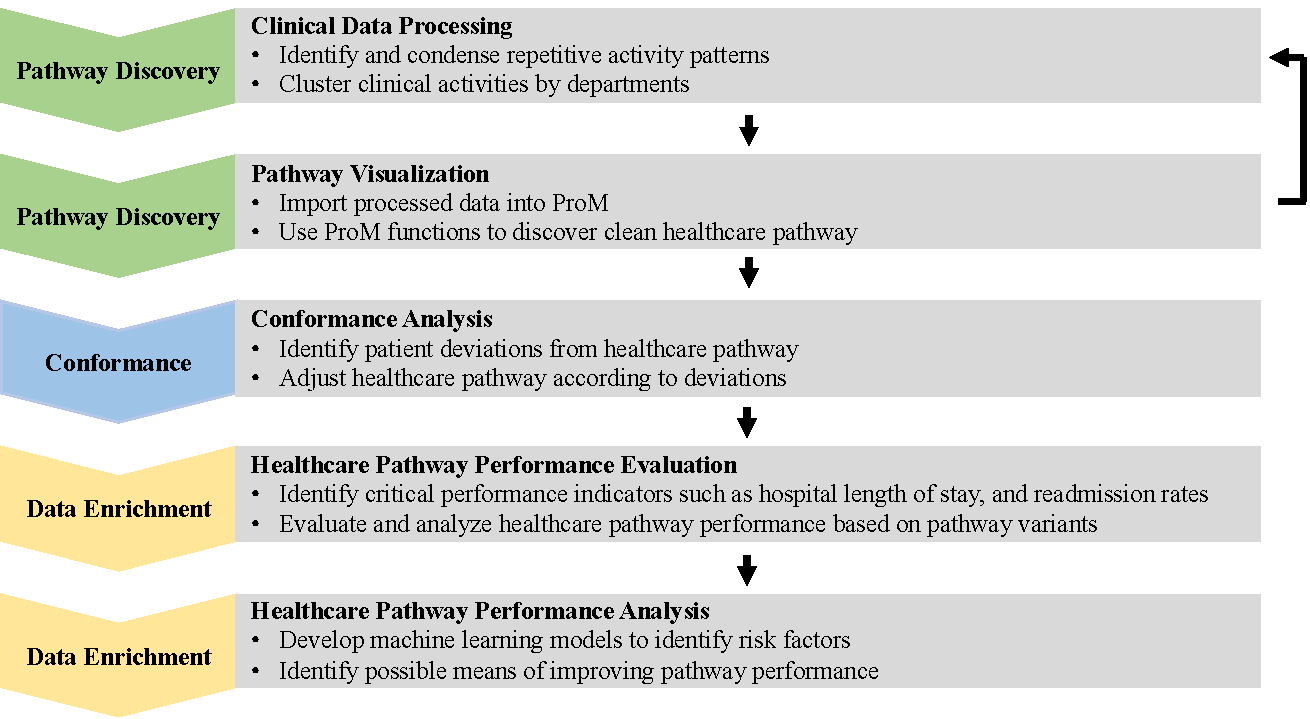
\includegraphics[width=\textwidth]{images/pipeline_diagram_journal.pdf}
\caption{The process mining pipeline comprises three sections, which
  are subdivided into five steps: Clinical data processing, pathway
  visualization, conformance analysis, healthcare pathway conformance
  evaluation, and prescriptive analytics of healthcare pathways. The
  first three steps are connected in two iterative cycles.}
\label{fig:pipeline}
\end{figure}

This study evaluates ProM (version 6.7) as the main process mining tool\footnote{\url{http://www.promtools.org}}. 
ProM is an open-source process mining software that is effective for construction of business models from input data files. ProM is chosen for this study because it has an intuitive user interface and supports many process mining plug-ins \cite{VanDongen2005}. The process mining and conformance analysis plug-ins supported by ProM are well documented. All these features of ProM make it easy for the process mining steps in the pipeline (see Fig.~\ref{fig:pipeline}) to be repeated by users with no background in process mining. The process mining techniques used in this paper are selected based on their ease for clinical interpretation and their potential to be combined with machine learning models. 

\subsection{Healthcare Pathway Discovery}
Healthcare pathway discovery is the first phase of the proposed process mining pipeline. It consists of two steps: clinical data processing and pathway visualization, which are conducted iteratively until a concise model is produced.
The aim is to use patient healthcare records stored in hospital information systems to design a concise pathway model that is easy for clinical interpretation. Therefore, clinical input is critical to the selection of appropriate processing methods. 
 
Healthcare pathways generally have much higher levels of complexity than standard business processes, and unprocessed clinical data contains too many clinical variations for a clean and concise pathway model to be mined \cite{Huang2013, Veiga2010}. Each pathway variant is a unique event sequence of a complete patient trace. The ProM plug-in \plugin{Explore Event Log} (from the Log Enhancement package) extracts pathway variants from patient traces, and the total number of pathway variants is an indicator of the level of clinical variation between patient traces. The basic format of an example pathway variant extracted by \plugin{Explore Event Log} is demonstrated in  Fig.~\ref{fig:example pathway variant}.

\begin{figure}[t]
\centering

\includegraphics[width=\textwidth]{images/example_pathway_variant_format2.jpg}
\caption{Basic format of example pathway variant visualized by ProM's
  plugin \plugin{Explore Event Log}. The same colour represents the same activity, and each activity is composed of a start event and a stop event.}
\label{fig:example pathway variant}
\end{figure}

In order to reduce healthcare pathway variations to a meaningful pathway model, the pathway variants visualized by the plug-in \plugin{Explore Event Log} are examined closely to determine the most suitable processing methods. 
There are three effective methods for reducing clinical variations without filtering patient traces:

\begin{description}
    \item[Cluster clinical activities] that are similar in nature so that the range of activities is reduced to a manageable size, e.g., `Abdomen CT scan' and `Pelvis CT scan' could be clustered into a single activity under `CT scan'.
    \item[Merge consecutive clinical activities] that are performed consecutively into a single activity, e.g., a patient receiving the same medication five times on the same day could be regarded as a single activity.
    \item[Condense repetitive activity patterns] 
         that repeat but exhibit variable cycle length. These patterns indicate an activity that must be performed periodically while the patient is waiting for a different activity to begin, e.g., lab tests to monitor a patient’s condition, medication to prevent infection. These repetitive patterns could be condensed into a single, parallel activity.
\end{description}
Clinical input is highly recommended at this step particularly for complex or unfamiliar healthcare pathways. 

%\subsubsection{Pathway Visualization}

\subsection{Healthcare Pathway Conformance Analysis}
It is very difficult for clinicians to manually track individual patient traces through the treatment process and ensure that they are conforming to standard protocols. Identifying unwarranted deviations and making the required interventions early in the process has the potential to improve health outcomes and decrease cost. 
Conformance analysis identifies patient deviations by comparing the pathway model to clinical data. 
Accuracy of the discovered healthcare pathway model is validated if the majority of the patient traces conform to the model. Patient traces rarely all follow identical pathways, so the healthcare pathway model is not expected to capture all patient traces. The objective is to discover a healthcare pathway model that captures the fundamental structure of most patient traces and detect unexpected patient deviations. 

ProM offers tools for conformance analysis of healthcare
pathway models: Its plug-in \plugin{Inductive Visual Miner} compares
patient traces from input clinical data to a healthcare pathway model
and indicates patient traces which are deviating from the pathway
model.
For this purpose, the pathway model is visualized as a process tree,
which is a hierarchical map comprised of decision nodes and
tasks representing clinical activities
\cite{25a7fd818bf44606a903d9b78b95cdd3}.
Therefore, process trees enable the identification of pathway branches
throughout the healthcare pathway model (c.f. Sec~\ref{Sec:AppendicitisDiscoveryConformance}).

If valid patient traces deviate from a healthcare pathway model, 
adjustments are made to the model to improve patient conformance.
A typical example might be the introduction of a new form of
treatment, which has not been included into the model yet.
Including these findings into the model leads to an iterative approach
between pathway discovery and conformance analysis (Fig.~\ref{fig:pipeline}).
Conversely, conformance analysis can identify where invalid
patient traces deviate from the model and investigate the reason for
the discrepancy, e.g., clinicians following obsolete pathways or data errors.

\subsection{Healthcare Pathway Data Enrichment}
% \subsubsection{Healthcare Pathway Performance Evaluation}
Data enrichment of healthcare pathways is the third phase of the
discussed process mining pipeline (Fig.~\ref{fig:pipeline}).
It comprises two steps: Healthcare pathway performance evaluation and
healthcare pathway performance analysis.

The main objectives of evaluating healthcare pathway performance are
to understand the strengths and weaknesses of the current pathway design,
and to identify potential methods of improvement. Possible indicators
of healthcare pathway performance include waiting times of clinical
activities, hospital length of stay, recovery time, and readmission
rates \cite{Rotter2008_pathways}.
Most of these indicators can be calculated or estimated using standard clinical timestamps. Postoperative Length of Stay (PLS), which is measured from leaving operating theatre to discharge, can also be considered as patient recovery time.
For surgical healthcare pathways,  PLS is one of the critical indicators for evaluating healthcare pathway
performance \cite{Pearson2001_pathways}. 

Analysing the performance of healthcare pathways with respect to
pathway variants and other possible influencing factors like
demographics or patient specific pathway characteristics, e.g. surgery duration (SD), is the final step of the process mining pipeline
(Fig.~\ref{fig:pipeline}).
Due to the fact, that most pathway performance indicators do not
follow normal distributions, while exhibiting significant stochastic
volatility, neither classical hypotheses tests \cite{Goodman2008_p-value}, nor point-predicting
machine learning models are appropriate for analysing healthcare
pathways.
Instead, probabilistic machine learning models
\cite{Ghahramani2015_PML} are used for extracting interpretable models
from healthcare pathways (Sec.~\ref{sec:ML}).
For this purpose, feature engineering \cite{DongLiu2018_FE} from
the patients' pathway traces (e.g. SD, pathway variant),
demographics (e.g. age), as well as medical documentation like written
diagnosis, time series, or images become important.
In order to demonstrate this approach, the following case study
discusses a probabilistic machine learning model for PLS, which
takes into account pathway variants
(Sec.~\ref{Sec:AppendicitisDiscoveryConformance}), as well as demographics, and
SD (Sec.~\ref{sec:ML}).

\section{Case Study: Appendicitis and Cholecystitis Healthcare Pathways}
This section discusses the healthcare pathway discovery process for the appendicitis and cholecystitis case studies. For this purpose, two years’ worth of data
from 2015 to 2017 on 448 appendicitis patients and 52 cholecystitis patients have been analysed. These case studies are selected because clinicians confirmed they are relatively simple surgical pathways with clear start and end points.

\subsection{Data Description}
\label{Sec:DataDescription}
The patient records for both case studies were collected from North Shore Hospital in Auckland, New Zealand.
The data were de-identified and an ethics approval for this research was obtained. All data sets collected from the hospital's information system on appendicitis and cholecystitis patients are summarized in Tab.~\ref{table:data description table}. Theatre encounter is the system ID used to identify patient traces, and clinical activities are categorized by clinical departments (e.g. radiology, pharmacy). Unfortunately, patient demographics data is only available for appendicitis patients. These data sets are processed and imported into ProM for pathway discovery and conformance analysis.

\newcommand{\tabitem}{~~\llap{\textbullet}~~}

\begin{table}[t]
\centering
\caption{Description of all data sets collected from North Shore Hospital for the appendicitis and cholecystitis case studies.}
\label{table:data description table}
\begin{tabular}{lll}
  \hline
  \hline
EMR  &     Columns of Interest & Data Type  \\
\hline
Acute Theatre   &    \tabitem Theatre Encounter & String\\  &\tabitem Surgery Start Time & Datetime\\  &\tabitem Surgery End Time & Datetime\\  &\tabitem Into Theatre Time & Datetime\\  &\tabitem Out of Theatre Time & Datetime\\
  \hline
General Surgery   &    \tabitem Theatre Encounter & String\\  &\tabitem Admission Time & Datetime\\  &\tabitem Discharge Time & Datetime\\
  \hline
Radiology/Pharmacy   &    \tabitem Theatre Encounter & String\\  /Lab/Anesthesia & \tabitem Clinical Activity & String\\  &\tabitem Clinical Activity Start Time  & Datetime\\
  \hline
Patient    &    \tabitem Theatre Encounter & String\\(specific to appendicitis patients)  &\tabitem Patient Age & Integer\\  &\tabitem Patient Gender  & String\\  &\tabitem Patient Ethnicity  & String\\
  \hline
  \hline
\end{tabular}
\end{table}

\subsection{Appendicitis Pathway Discovery and Conformance Analysis}
\label{Sec:AppendicitisDiscoveryConformance}
The appendicitis pathway model, which has been generated by ProM's
plugin \plugin{Explore Event Log}, is shown in
Fig.~\ref{fig:appendicitis pathway variants} in the form of a pathway
variant plot.
The pathway variants are extracted without activities related to medication (i.e. preoperative and postoperative cefuroxime/metronidazole) because the clinicians confirmed that antibiotics are usually taken while the patient is waiting for surgery or discharge. The duration of these activities are therefore highly variable and result in a high number of unique pathway variants.

%The variant specific numbers of patient traces given in  Fig.~\ref{fig:appendicitis pathway variants} are repeated in Tab.~\ref{table:appendicitis variant table}.
The pathway variant plot visualizes the 13 pathway variants of the
appendicitis model sorted from the most common pathway (index 0) to
the least common pathway (index 12).
The top four variants account for approximately 88\% of the patient
traces (Tab.~\ref{table:appendicitis variant table}).
All clinical activities are represented by a start event and a stop
event.
The activities are colour coded such that the same colour refers to the same clinical activity. The most common pathway variant (index 0) only consists of anesthesia and surgery, while the second most common variant (index 1) also includes preoperative X-ray.
The pathway variant indices are used in Sec.~\ref{sec:ML} as one-hot
encoded feature of the probabilistic machine learning model.

\begin{figure}[t]
\hspace{-2cm}
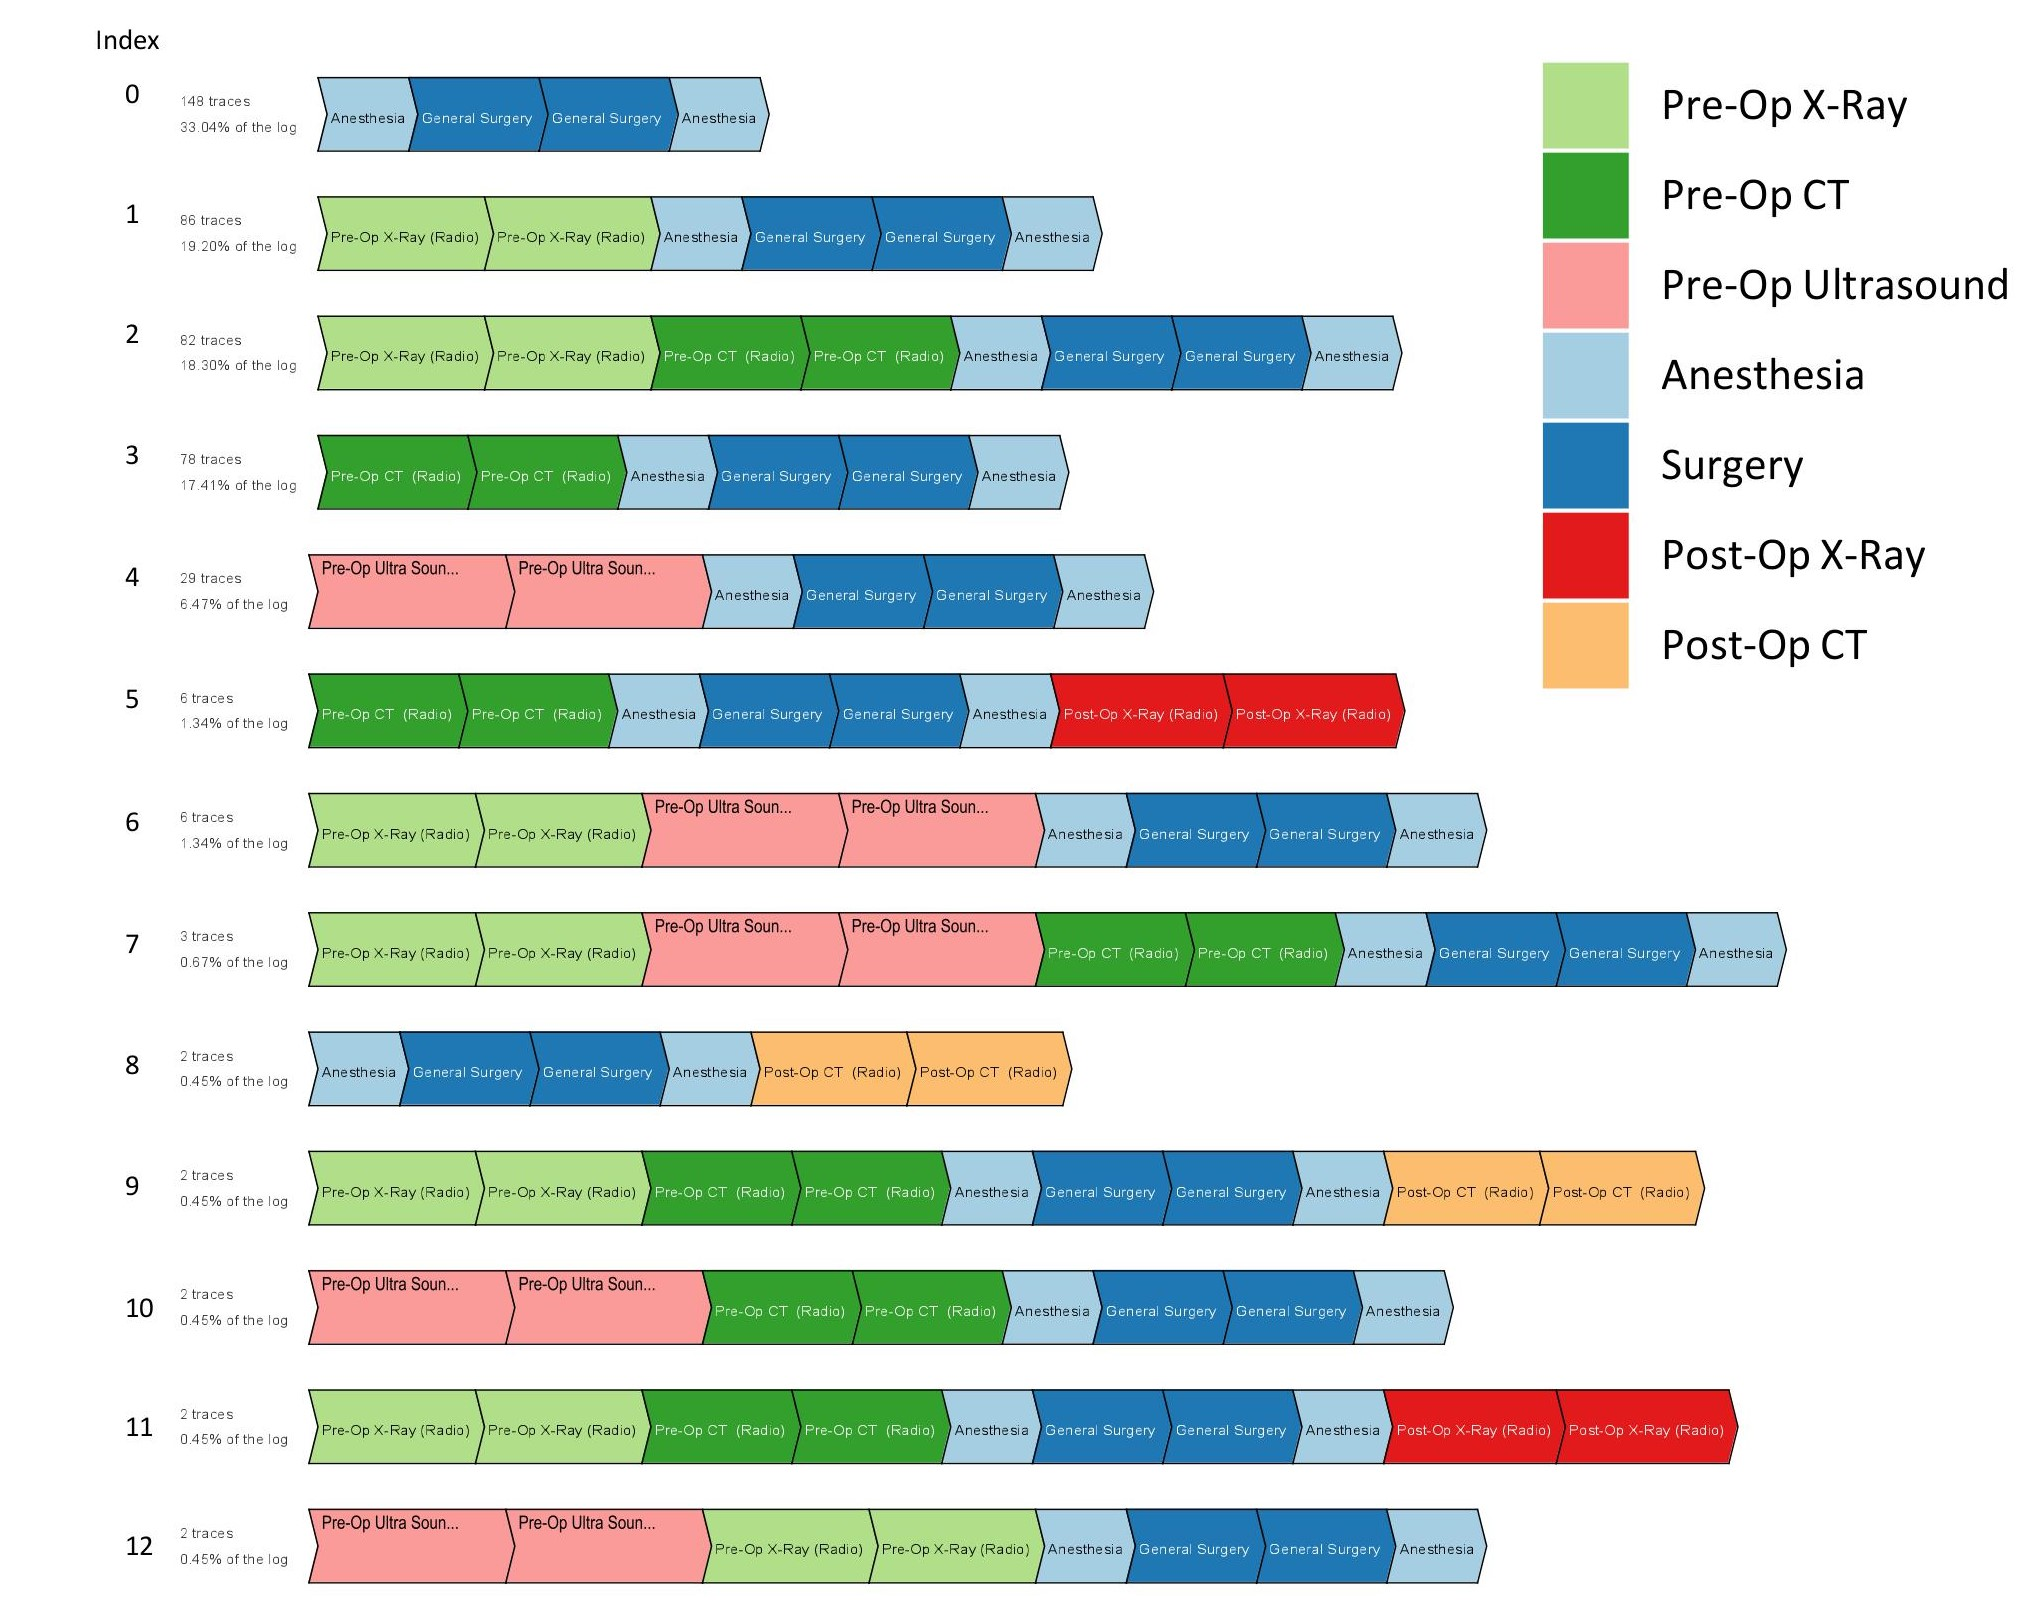
\includegraphics[width=1.5\textwidth]{images/appendicitis_variant_index_anes.jpg}
\caption{Appendicitis pathway variant plot auto-generated by ProM's
  plugin \plugin{Explore Event Log}. 
  The plot visualizes the sequences of start and stop events for the different pathways.
  For the purpose of readability the legend was added and the
  statistics on the left are repeated in Tab.~\ref{table:appendicitis variant table}.
 The top four variants account for approximately 88\% of the patient
 traces. They are modelled as one-hot encoded features V0, V1, V2, and V3
 in Sec.~\ref{sec:ML}, while pathway variants V4--V12 together represent
 the base model.
 }
\label{fig:appendicitis pathway variants}
\end{figure}
\clearpage

\begin{table}[t]
\centering
\caption{Statistics of appendicitis patient traces shown in Fig.~\ref{fig:appendicitis pathway variants}.}
\label{table:appendicitis variant table}
\begin{tabular}{llllllll}
  \hline
  \hline
Variant &     0  &     1  &     2  &     3  &    4  &    5  &    6  \\
\hline
Patients   &    148 &     86 &     82 &     78 &    29 &     6 &     6 \\
  Percentage &  33.04\% &  19.20\% &  18.30\% &  17.41\% &  6.47\% &  1.34\% &  1.34\%\\
  \hline
  \hline
Variant &     7  &    8  &    9  &    10 &    11 &    12 \\
\hline
Patients   &   3 &     2 &     2 &     2 &     2 &     2 \\
Percentage &  0.67\% &  0.45\% &  0.45\% &  0.45\% &  0.45\% &  0.45\% \\
  \hline
  \hline
\end{tabular}
\end{table}

The first stage of the appendicitis pathway model visualized by \plugin{Inductive Visual Miner} is shown in Fig.~\ref{fig:ivm pathway model example}.
Unlike the pathway variants, this appendicitis pathway model incorporates activities representing antibiotics. The model indicates that 42 patients perform ultrasound and 183 patients perform X-ray upon admission. 

\begin{figure}[t]
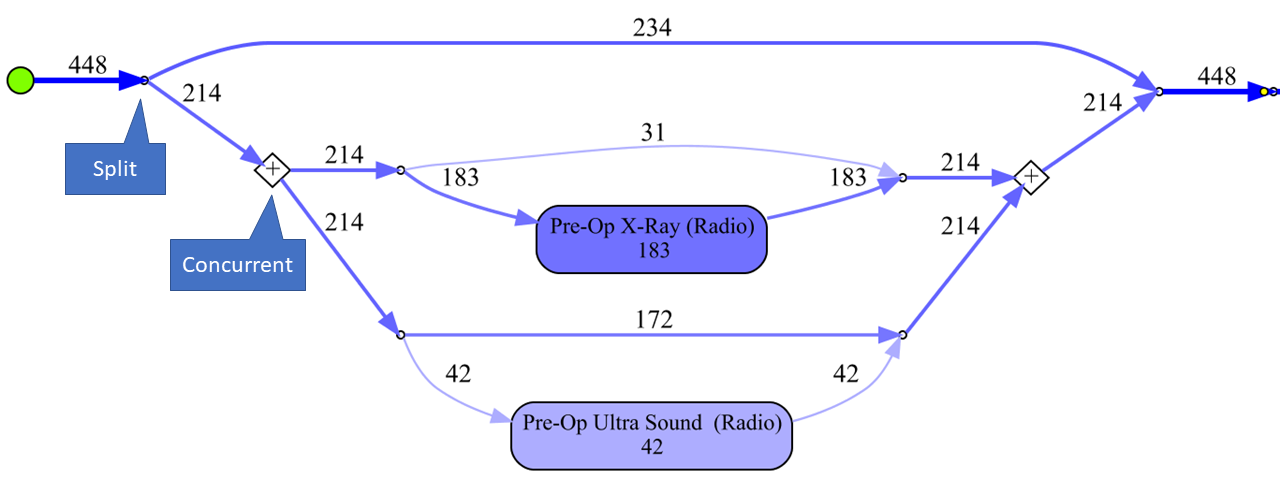
\includegraphics[width=\textwidth]{images/ivm_appendicitis_first_stage_example.png}
\caption{First stage of the appendicitis pathway model generated by
  ProM. The following stages have been omitted for the purpose of
  readability.
  The process indicates that 234 patients do not have any preoperative
  imaging diagnostics, while 214 patients enter the imaging
  diagnostics branch.
  Please refer to Leeman's manual on \plugin{Inductive Visual Miner} for details on the model notations \cite{leemansinductive}.}
\label{fig:ivm pathway model example}

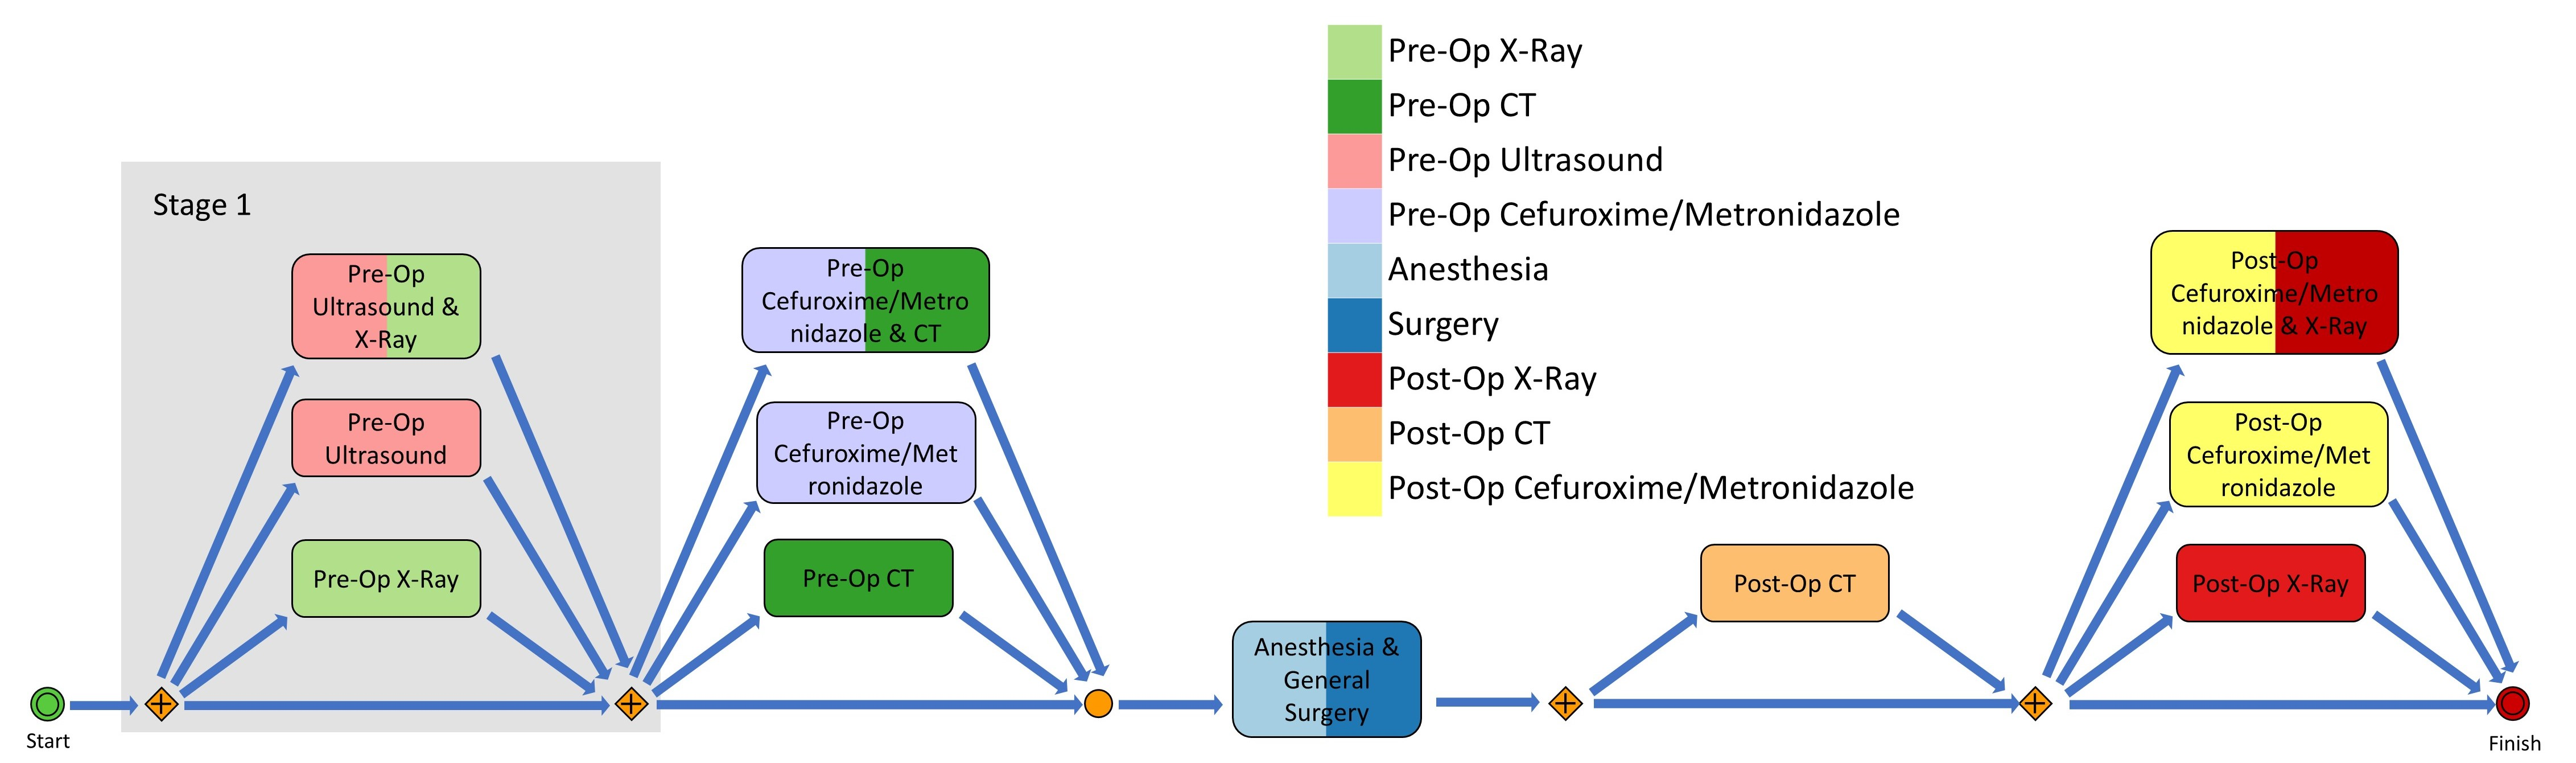
\includegraphics[width=\textwidth]{images/communicative_appendicitis_process_models_anes.jpg}
\caption{Appendicitis pathway model using nomenclature of Tab.~\ref{table:notation table}. All preoperative and
  postoperative activities belong to radiology and pharmacy
  departments. Preoperative antibiotics are taken in the second stage
  of the treatment pathway.}
\label{fig:appendicitis pathway model}
\end{figure}

While the complex process tree notation of ProM's \plugin{Inductive
  Visual Miner} plugin is optimal for detailed analysis, it has been
reformulated under new notations for easy clinical interpretation.
The new model notations are summarized in Table \ref{table:notation
  table}, and the reformulated appendicitis pathway model is shown in
Fig.~\ref{fig:appendicitis pathway model}. The section of the model
labelled as `Stage 1' in Fig.~\ref{fig:appendicitis pathway model}
corresponds to the process tree shown in Fig.~\ref{fig:ivm pathway
  model example}.
This is the final pathway model that has been compiled based on
clinical input to account for valid patient deviations, and all
patient traces conform to the updated pathway.
The most common pathway variant (index 0) shown in Fig.~\ref{fig:appendicitis pathway variants} corresponds to the horizontal path from start to finish in Fig.~\ref{fig:appendicitis pathway model}.

\begin{table}[t]
\centering
\caption{Definitions of new pathway model notations.}
\label{table:notation table}
\begin{tabular}{ l c l }
 \hline
 \hline
 Notation & Symbol & Definition \\ 
 \hline
 Orange Diamond 
 &
%\raisebox{-\totalheight}{\includegraphics[width=0.3\textwidth, height=60mm]{images/myLboro.png}}
 \raisebox{-3pt}{
\includegraphics[width=0.5cm]{images/decision_node.png}}
 & Decision Point, indicating exclusive choice \\ 
 \hline
 Orange Connector 
 & 
 \raisebox{-3pt}{
\includegraphics[width=0.5cm]{images/connection_node.png}}
 & Pathway Connection Point \\
 \hline
 Green Connector 
 & 
 \raisebox{-3pt}{
\includegraphics[width=0.5cm]{images/start_node.png}}
 & Starting Point \\
 \hline
 Red Connector 
 & 
 \raisebox{-3pt}{
\includegraphics[width=0.5cm]{images/finish_node.png}} 
 & Finishing Point \\
 \hline
 \hline
\end{tabular}
\end{table}

\subsection{Length of Stays of Appendicitis Pathway Variants}
Length of stays in hospital are analyzed based on the 13 identified appendicitis pathway variants shown in Fig.~\ref{fig:appendicitis pathway variants}. Hospital length of stay, measured from admission to discharge, for each of the 13 appendicitis pathway variants are shown in Fig.~\ref{fig:hospital length of stay appendicitis}. Postoperative length of stay, measured from leaving theatre to discharge, for each pathway variant is shown in Fig.~\ref{fig:post op length of stay appendicitis}. Pathway variant 9 has the longest length of stay for both measures. Pathway variants 5, 7 and 11 also have relatively long length of stays. Out of these four pathway variants, only pathway variant 7 consists of no postoperative activities. The number of patient traces that follow each pathway variant is limited, and more samples are required to identify rate-determining steps. Probabilistic machine learning models are used to further investigate factors influencing postoperative length of stay (Sec.~\ref{sec:ML}).

\begin{figure}[t]
\centering
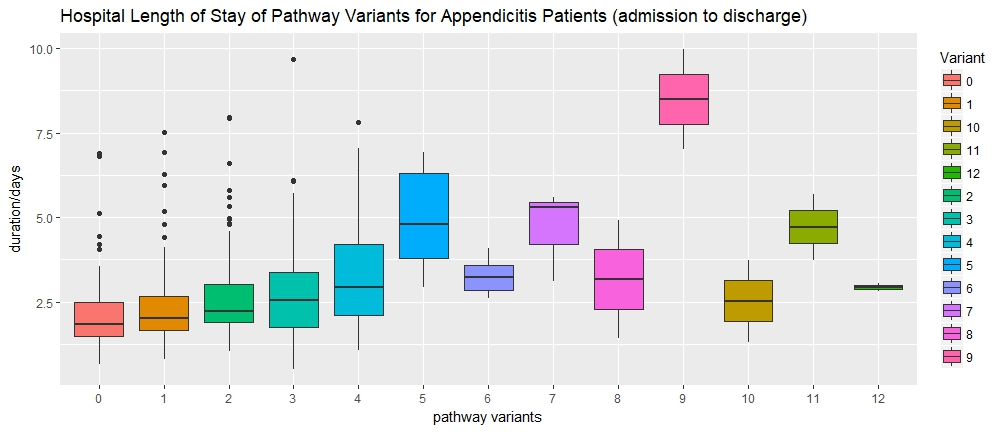
\includegraphics[width=\textwidth]{images/hospital_length_of_stay_appendicitis_210518.jpeg}
\caption{Hospital length of stay of the 13 appendicitis pathway variants, measured from admission to discharge.}
\label{fig:hospital length of stay appendicitis}
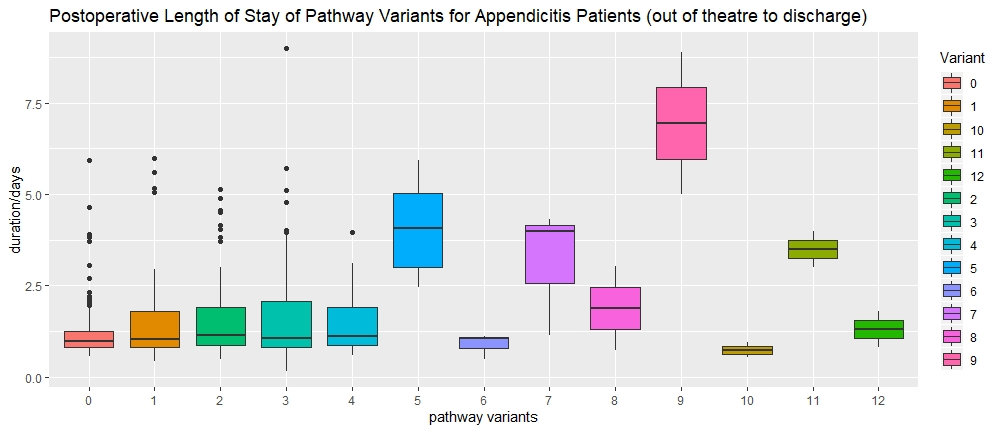
\includegraphics[width=\textwidth]{images/postoperative_length_of_stay_appendicitis.jpeg}
\caption{Postoperative length of stay of the 13 appendicitis pathway variants, measured from leaving theatre to discharge.}
\label{fig:post op length of stay appendicitis}
\end{figure}

\subsection{Cholecystitis Pathway Discovery and Conformance Analysis}
\label{Sec:CholecystitisDiscoveryConformance}
This section shows the cholecystitis pathway variant plot auto-generated by ProM. Cholecystitis pathway variants are analyzed without activities from the `antibiotics' sub-process and the `monitoring labs' sub-process (see Fig.~\ref{fig:cholecystitis pathway model} for the activities from the two sub-processes). Clinicians confirmed that these sub-processes are standard monitoring and maintenance systems while the patient is waiting for further diagnosis. Only analyzing activities from the primary cholecystitis pathway significantly reduces the level of clinical variation between patient traces.

The cholecystitis pathway model consists of 10 pathway variants. The 10 pathway variants of the cholecystitis pathway model are shown in Fig.~\ref{fig:cholecystitis pathway variants}, and the number of patient traces that follow each pathway variant are listed in Table \ref{table:cholecystitis variant table}. Pathway variants from Fig.~\ref{fig:cholecystitis pathway variants} are sorted from the most common pathway (index 0) to the least common pathway (index 9). The most common pathway variant (index 0) consists of anesthesia, surgery, and surgical pathology lab. The second pathway variant (index 1) includes surgery without anesthesia because of faulty clinical data. 

\begin{figure}[t]
\hspace{-2cm}
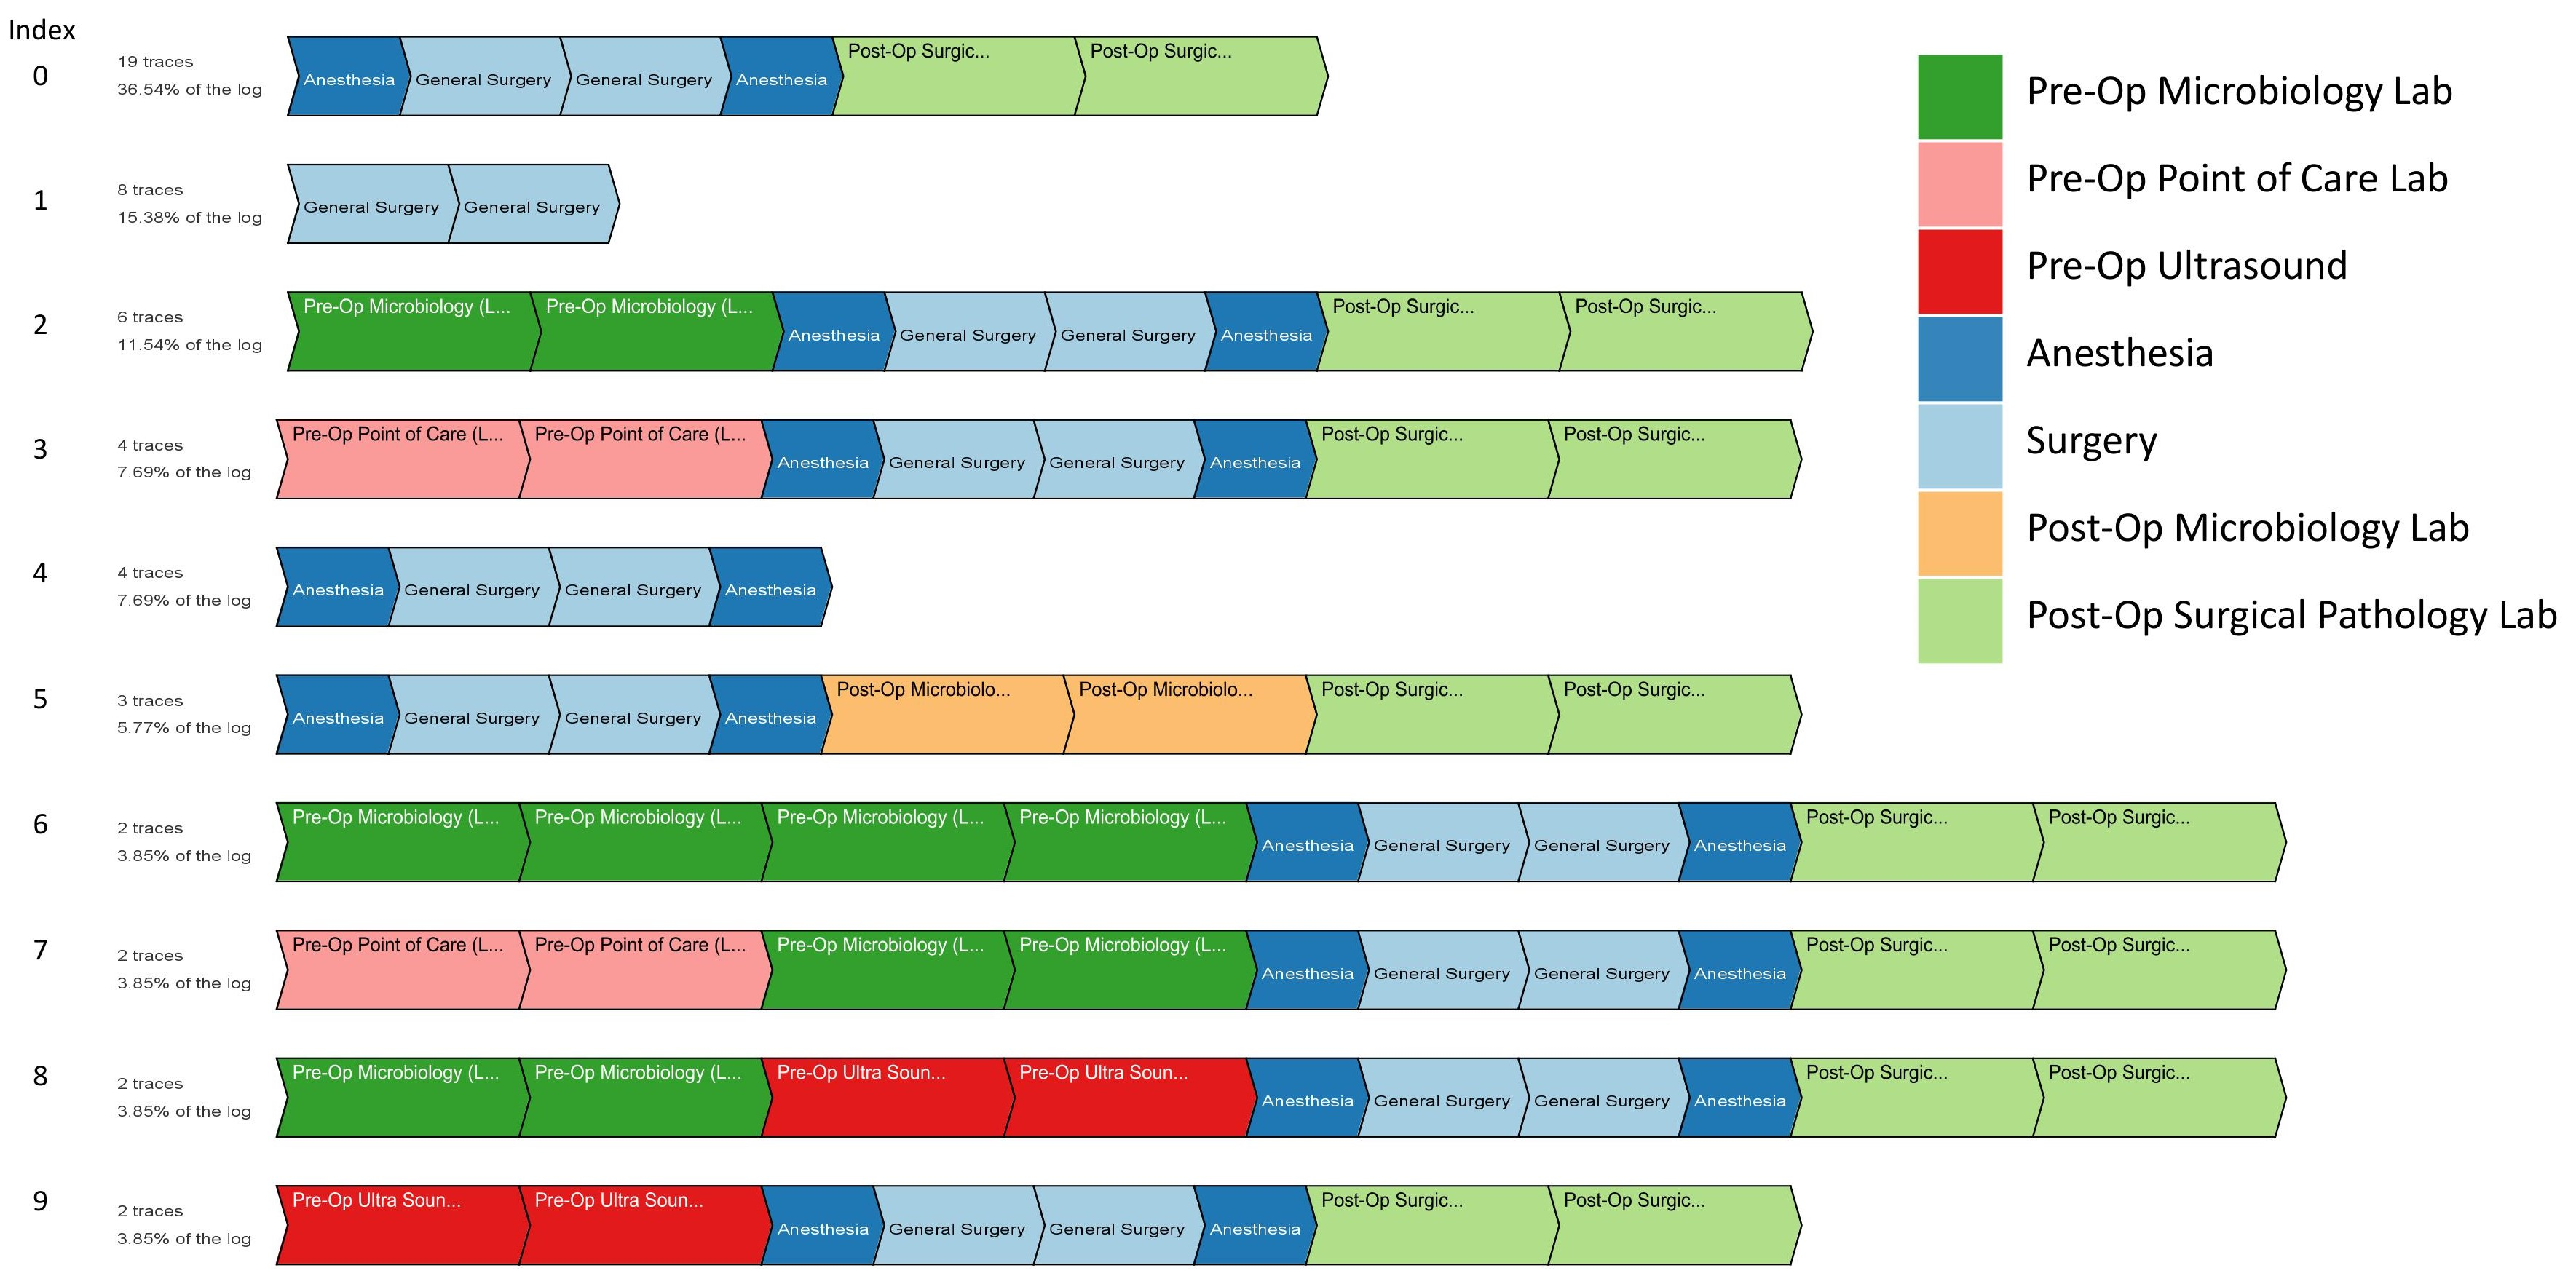
\includegraphics[width=1.5\textwidth]{images/cholecystitis_variant_index_anes.jpg}
\caption{Cholecystitis pathway variant plot auto-generated by ProM's plugin \plugin{Explore Event Log}. For the purpose of readability the legend was added and the statistics on the left are repeated in Tab.~\ref{table:cholecystitis variant table}.
The top three variants account for approximately 63\% of the patient traces.}
\label{fig:cholecystitis pathway variants}
\end{figure}

\begin{table}[t]
\centering
\caption{Statistics of cholecystitis patient traces shown in Fig.~\ref{fig:cholecystitis pathway variants}.}
\label{table:cholecystitis variant table}
\begin{tabular}{llllll}
  \hline
  \hline
Variant &     0  &     1  &     2  &     3  &    4\\
\hline
Patients   &    19 &     8 &     6 &     4 &    4\\
  Percentage &  36.54\% &  15.38\% &  11.54\% &  7.69\% &  7.69\%\\
  \hline
  \hline
Variant &     5  &    6  &    7  &    8 &    9\\
\hline
Patients   &   3 &     2 &     2 &     2 &     2 \\
Percentage &  5.77\% &  3.85\% &  3.85\% &  3.85\% &  3.85\% \\
  \hline
  \hline
\end{tabular}
\end{table}

The cholecystitis pathway model visualized by \texttt{`Inductive Visual Miner'} incorporates activities from the `antibiotics' sub-process and the `monitoring labs' sub-process. A breakdown of the cholecystitis pathway model into one primary pathway and two concurrent sub-processes is shown in Fig.~\ref{fig:cholecystitis pathway model}, and the model notations are summarized in Table \ref{table:notation table}. The first pathway model in Fig.~\ref{fig:cholecystitis pathway model} is the primary pathway, followed by the `antibiotics’ sub-process and the `monitoring labs’ sub-process. Patient traces can execute any combination of the two sub-processes concurrently with the primary pathway. Based on this model, preoperative haematology and chemistry labs tend to span the entire preoperative process, while preoperative antibiotics are taken closer to surgery. The eight patient traces that follow the second pathway variant (index 1) do not conform to this pathway model because of faulty clinical data. These eight patients suffer from both appendicitis and cholecystitis. Appendicitis and cholecystitis are studied as separate healthcare pathways in this study, and activity ‘Anesthesia’ is only recorded in the appendicitis data sets for the eight patients that suffer from both appendicitis and cholecystitis. This demonstrates that conformance analysis is able to detect flaws in the hospital's information system.

\begin{figure}[t]
\centering
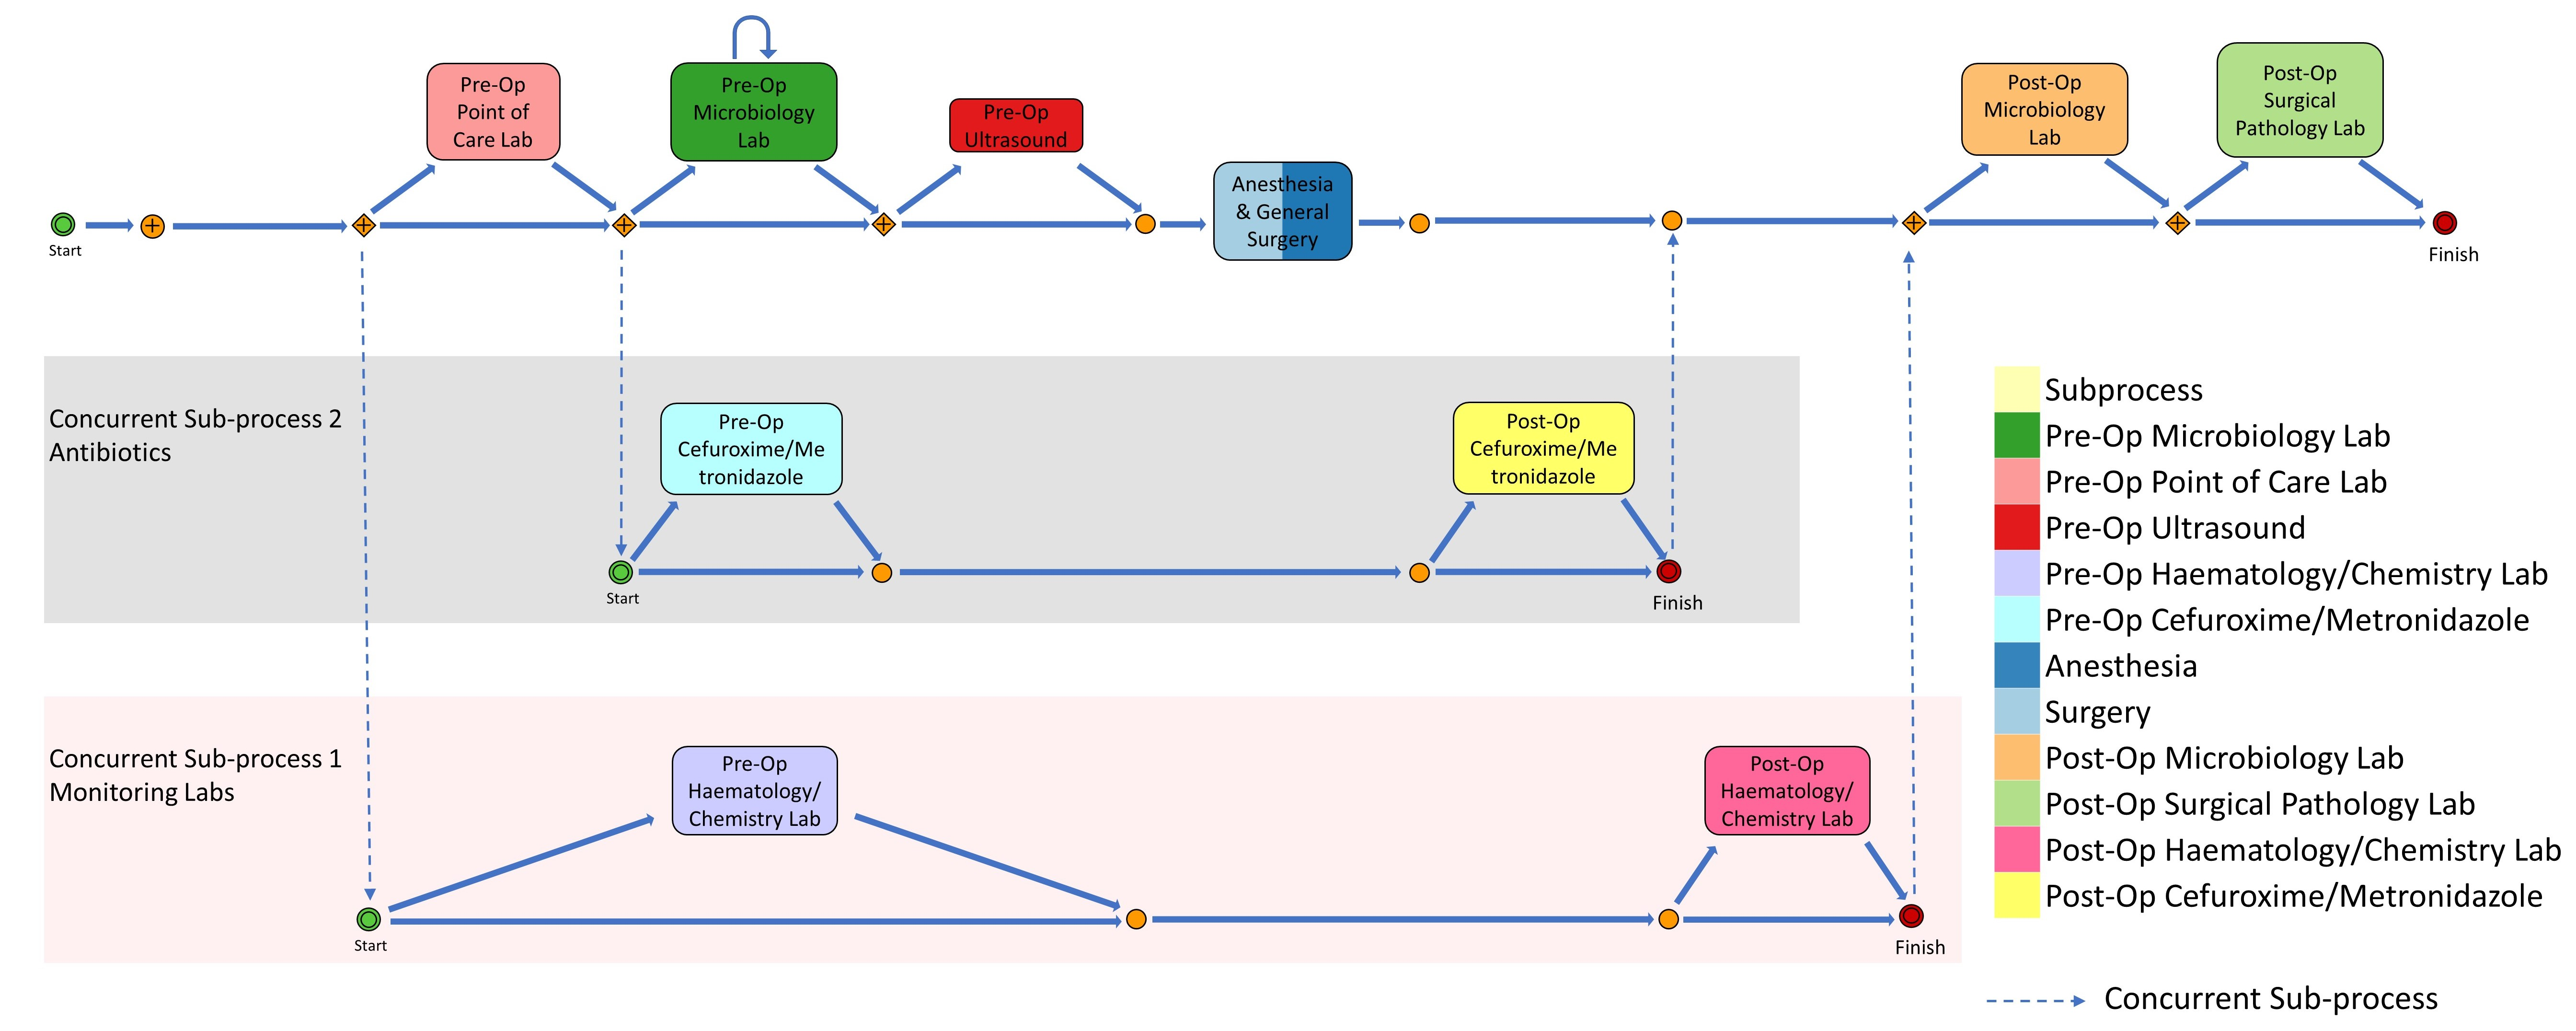
\includegraphics[width=18cm,angle=270]{images/communicative_cholecystitis_process_models_anes.jpg}
\caption{Cholecystitis pathway model using nomenclature of Tab.~\ref{table:notation table}. The model is broken down into one primary pathway and two sub-processes.}
\label{fig:cholecystitis pathway model}
\end{figure}

\subsection{Length of Stays of Cholecystitis Pathway Variants}
Length of stays are analyzed based on the 10 identified cholecystitis pathway variants shown in Fig.~\ref{fig:cholecystitis pathway variants}. Hospital length of stay, measured from admission to discharge, for each of the 10 cholecystitis pathway variants are shown in Fig.~\ref{fig:hospital length of stay cholecystitis}. Postoperative length of stay, measured from leaving theatre to discharge, for each pathway variant is shown in Fig.~\ref{fig:post op length of stay cholecystitis}. Pathway variant 1 appears to have the longest total postoperative length of stay even though it consists of no postoperative activities. All patients that follow pathway variant 1 suffer from both appendicitis and cholecystitis, and the clinicians confirmed that the long total postoperative length of stay could be due to a prolonged recovery time.  

\begin{figure}[t]
\centering
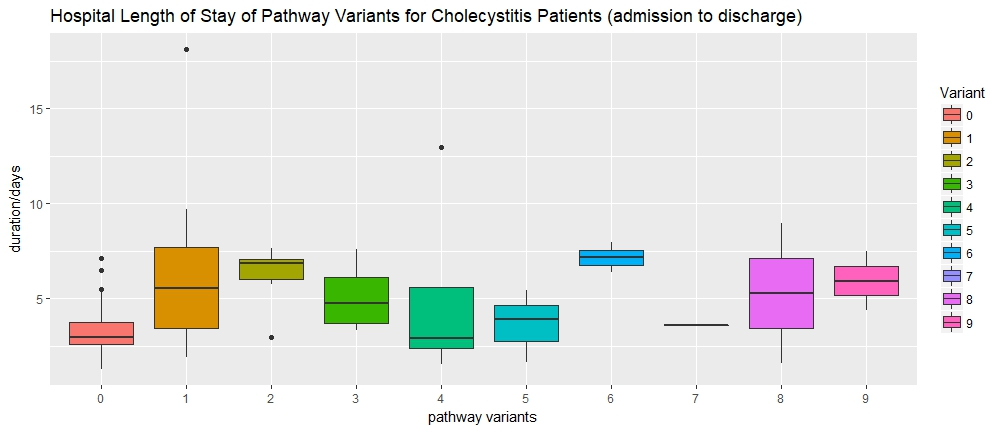
\includegraphics[width=\textwidth]{images/hospital_length_of_stay_cholecystitis_210518.jpeg}
\caption{Hospital length of stay of the 10 cholecystitis pathway variants, measured from admission to discharge.}
\label{fig:hospital length of stay cholecystitis}
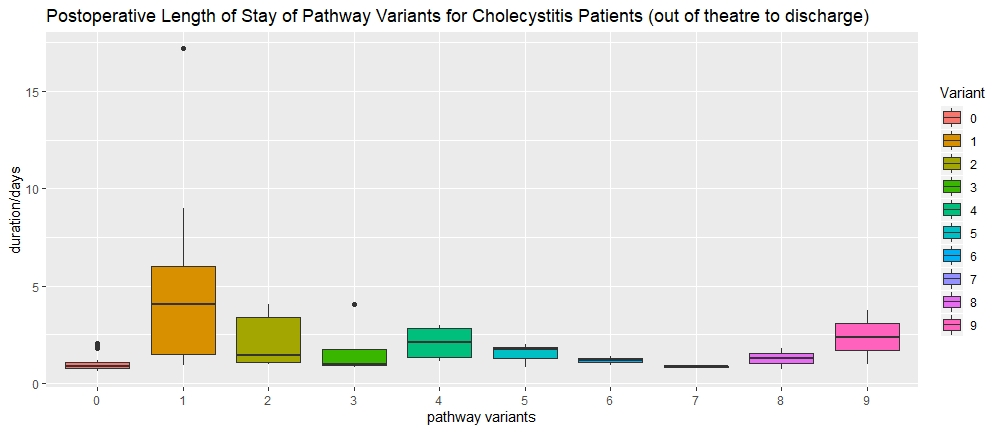
\includegraphics[width=\textwidth]{images/postoperative_length_of_stay_cholecystitis.jpeg}
\caption{Postoperative length of stay of the 10 cholecystitis pathway variants, measured from leaving theatre to discharge.}
\label{fig:post op length of stay cholecystitis}
\end{figure}

\subsection{Probabilistic Machine Learning Model for Postoperative Length of Stay of Appendicitis Patients}
\label{sec:ML}
The following section investigates the question of whether the pathway
variants of the appendicitis case study are relevant features or
covariates for explaining the stochastic volatility of PLS (Fig.~\ref{fig:Geom}a).
This is quite a challenging task, because the individual healing process is expected to depend on personal factors like age \cite{polanczyk2001impact} as well as the individual severity of the appendicitis inflammation, which in general is unknown at this stage of the data analysis, but might be captured by proxies like surgery duration (SD). As mentioned in Sec.~\ref{Sec:DataDescription}, demographics data on cholecystitis patients is unavailable so probabilistic models are only built for appendicitis patients.

\begin{figure}
  \centering
  \begin{tabular}{ll}
    (a) & (b) \\
    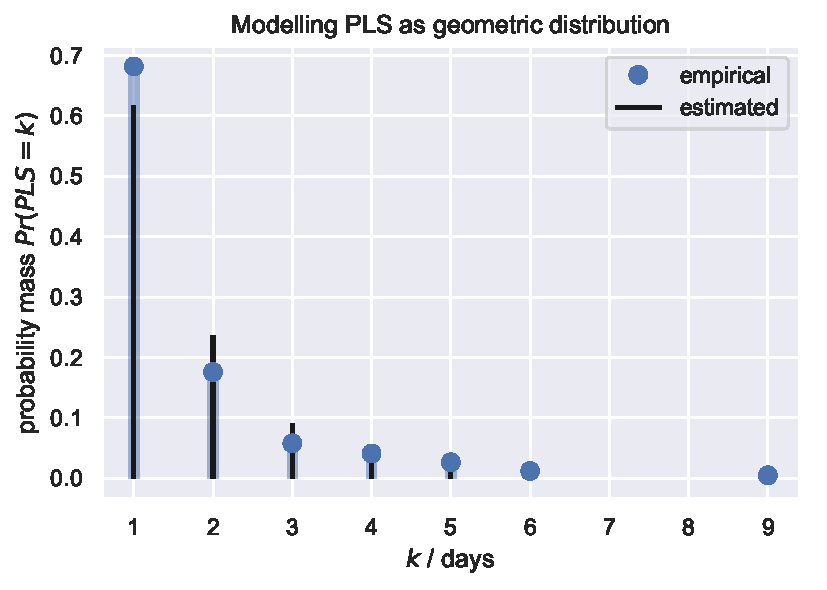
\includegraphics[width=0.5\textwidth]{images/DS19eH1_G0__empirical_geometric.pdf}
    &
    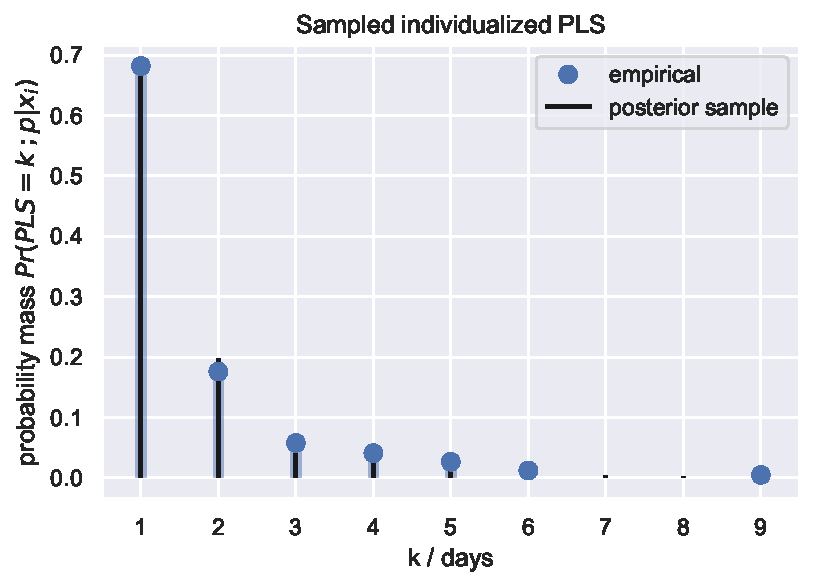
\includegraphics[width=0.5\textwidth]{images/DS19fk1_c0__sampled_posterior.pdf}\\
  \end{tabular}
    \caption{Modelling PLS as geometric distribution without patient
      specific model (a) and with individualised posterior (b) from
      model B (Eq. \eqref{modelB}). Sampling from patient specific
      posterior distributions replicates the observed PLS quite well.
      }
    \label{fig:Geom}
\end{figure}

For the purpose of this analysis, patients' traces with complete
demographic information (415 samples) are selected and
the patients' $PLS$, which is
calculated as the time interval between leaving operating theatre and discharge, is
converted into the number of days after surgery. Therefore, a $PLS$ of
one corresponds to a patient who has been discharged the day after
surgery. Three of the $N=415$  %DS19fA0
patient traces had a PLS of zero, because the surgery ended shortly after midnight and the patients were discharged on the same day. In order to simplify our analysis, the interpretation of PLS was broadened to the number of night rests after surgery, such that the PLS of these three patients could be projected to one.

Analysing the PLS of the 415 appendicitis patients reveals a
histogram which closely resembles a Geometric distribution (Fig.~\ref{fig:Geom}a)
\begin{equation}
Pr(PLS=k) = \text{Geom}(k; p) = (1-p)^{k-1}p^{k},
\end{equation}
parameterized by probability $p$ of being discharged on the $k^\text{th}$ day, respectively $k$ nights of rest after surgery. 
However, estimating $p$ as inverse mean of the observed PLS to 
\begin{equation}
 \hat{p} = \frac{N}{\sum\limits_{i=1}^N PLS_i} \approx 61.8\%	
\end{equation}
reveals that the average discharge probability $\hat{p}$ does not
generalize well over the cohort (Fig.~\ref{fig:Geom}a), because the number of patients being discharged on the first day after surgery is underestimated and the number of patients being discharged on the second and third day after surgery is overestimated.

For the following probabilistic machine learning models, the individualized discharge probability $p_i$ is modelled as a generalized linear model (GLM) using the inverse logistic function (logit) as a link function and the geometric distribution for generating the likelihood. 
For the following analysis, we are comparing two different models of
discharge probability $p_i$ as
\begin{equation}\label{modelA}
  \begin{split}
  \text{logit}(p_i) \sim & \;SD_i + \text{log}(age_i) + 
                            V_{0,i} + V_{1,i} + V_{2,i} + V_{3,i} + V_{0,i}\times\text{log}(age_i) +\\
  &   V_{1,i}\times\text{log}(age_i) + V_{2,i}\times\text{log}(age_i) + V_{3,i}\times\text{log}(age_i),\\
  \end{split}
\end{equation}
which we refer to as \textit{model A}, and
\begin{equation}\label{modelB}
  \begin{split}
  \text{logit}(p_i) \sim & \;SD_i + \text{log}(age_i) +
                                                         V_{0,i} + V_{1,i} + V_{2,i} + V_{3,i} + V_{0,i}\times\text{log}(age_i) +\\
  &    V_{1,i}\times\text{log}(age_i),\\
  \end{split}
\end{equation}
which we refer to as \textit{model B}.
These two models have been selected because they were the most
credible based on the widely applicable information criterion
(WAIC) and leave-one-out cross-validation (LOO) statistics
\cite{Vehtari2017_WAIC_LOO}.
The explanatory variables $V_{j,i}$ are categorical with 
\begin{equation}
V_{j,i} = \begin{cases}
	1: & V_{j,i} = j,\\
        0: & \text{otherwise}.
\end{cases}
\end{equation}
Therefore, the case $V_{0,i}=V_{1,i}=V_{2,i}=V_{3,i}=0$ corresponds to variants V4--V12 of Fig.~\ref{fig:appendicitis pathway variants}.
Models A and B make the simplifying assumption that the individualised
probability of discharge $Pr(PLS_i=k|x_i)$ can be estimated from 
\begin{equation}
x_i = (SD_i, \text{log}(age_i), V_{0,i}, V_{1, i}, V_{2, i}, V_{3, i}).
\end{equation}
 being available at the end of surgery, when future treatment steps and therefore the complete pathway variant for the respective $i^\text{th}$ patient have been decided on:
\begin{equation}
\begin{split}
Pr(PLS_i=k|x_i) & = \text{Geom}\left(k;p(x_i)\right) \\
& = \left(1-p(x_i)\right)^{k-1}\left(p(x_i)\right)^{k} \\
%& = \left(1-\mathbb{E}_{x_i}[p]\right)^{k-1}\left(\mathbb{E}_{x_i}[p]\right)^{k} \\
          %        & = \left(1-\text{logistic}(f(x_i))\right)^{k-1}\text{logistic}(f(x_i))^{k} \\
          %        & = \left(1+e^{f(x_i)}\right) \left(2 + e^{-f(x_i)} + e^{f(x_i)}\right)^{-k}
\end{split}
\end{equation}
with $p(x_i)$ being modelled either by Eq. \eqref{modelA} or
\eqref{modelB}.
    
The statistical model has been fitted using PyMC3
\citep{Salvatier2016_PyMC3} version 0.24.2 using the No-U-Turn Sampler
(NUTS) with 20,000 samples, 2,000 tuning steps, 2 chains, and an
acceptance rate of 90\%. The 95\% credible intervals of the estimated
model coefficients are shown in Fig.~\ref{fig:forest_plots}. The
Gelman-Rubin convergence statistic Rhat is close to one for all
coefficients (Tab.~\ref{tab:coeff}). 
However, for Model A the coefficients of the interaction terms
$\text{log}(age_i)\times V_2$ and $\text{log}(age_i)\times V_3$ are
close to zero with negative expectation values but a 25\% and 15\%
probability of being larger than zero (Tab.~\ref{tab:coeff}). 
Therefore, we have decided to focus the following analysis of the
fitted model on Eq.~\eqref{modelB} for which all credible intervals
exclude zero (Fig.~\ref{fig:forest_plots}b).
However, this does not change the overall trend depicted in Fig.~\ref{fig:posterior}.
It is important to note that both the coefficients of $SD$ and $\text{log}(age)$ are negative. This means that for the base model of variants V4--V12 as well as variants V2 and V3, the probability of discharge decreases with increasing SD and age. 
Compared to the base model, Variants V2 and V3 have a higher discharge probability because both coefficients are positive. 
The situation is more complicated for variants V0 and V1, because their coefficients are negative but the coefficients of their interaction terms with $\text{log}(age)$ are positive, which basically counterbalances the effect of $\text{log}(age)$.

\begin{figure}
  \centering
    \begin{tabular}{ll}
(a) Model A \eqref{modelA} & (b) Model B \eqref{modelB}\\
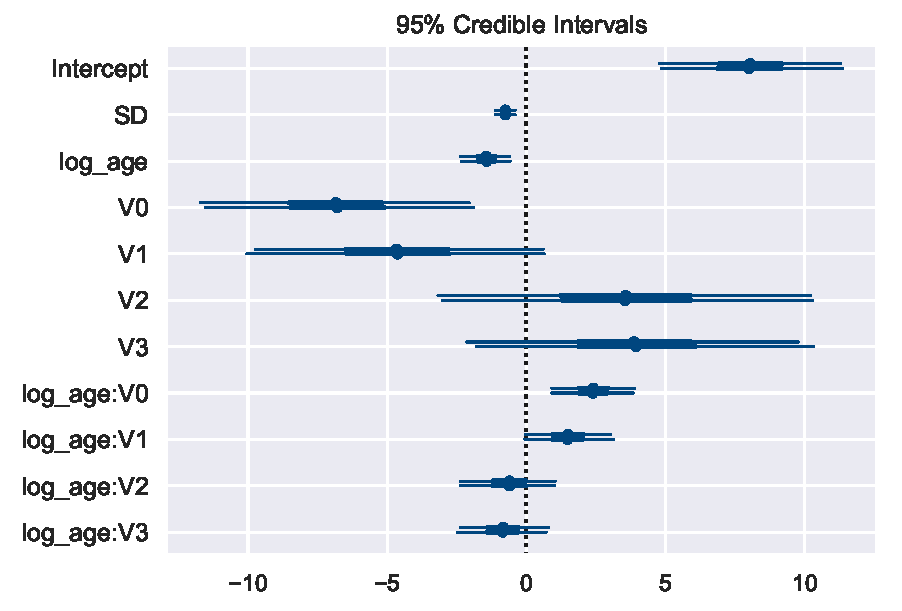
\includegraphics[width=0.5\textwidth]{images/DS19fm0_c0__forestplot_model_A.pdf}&
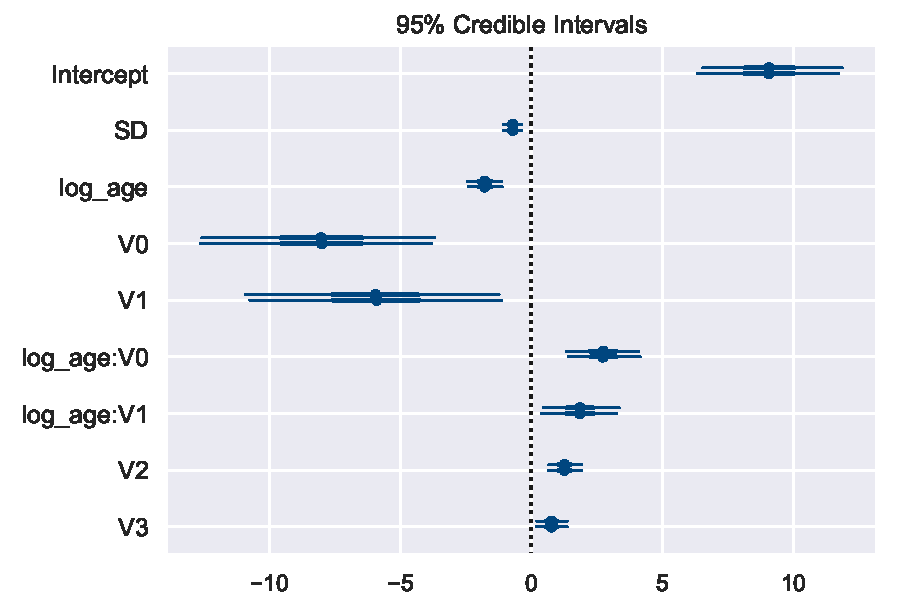
\includegraphics[width=0.5\textwidth]{images/DS19fk1_c0__forestplot_model_B}\\
\end{tabular}
    \caption{Credible intervals for models A \eqref{modelA} and B \eqref{modelB}.}
    \label{fig:forest_plots}
\end{figure}

\begin{table}
\caption{\label{tab:coeff} Coefficients of model B. Rhat is the
  potential scale reduction factor. A value of one indicates
  convergence.}
\centering
\begin{tabular}{lrrrr}
\hline
\hline
{} &      mean &    hpd\_2.5 &   hpd\_97.5 &      Rhat \\
\hline
Intercept  &  9.09 &   6.48 &  11.85 &  0.999988 \\
SD        & -0.71 &  -1.059 &  -0.371 &  0.999987 \\
log\_age    & -1.781 &  -2.46 &  -1.154 &  0.999988 \\
V0         & -8.04 & -12.56 &  -3.70 &  0.999980 \\
V1         & -5.95 & -10.82 &  -1.186 &  1.000013 \\
log\_age:V0 &  2.75 &   1.365 &   4.12 &  0.999980 \\
log\_age:V1 &  1.864 &   0.423 &   3.32 &  1.000013 \\
V2         &  1.267 &   0.646 &   1.901 &  1.000062 \\
V3         &  0.766 &   0.199 &   1.363 &  1.000046 \\
\hline
\hline
\end{tabular}
\end{table}


\begin{figure}
    \centering
    \begin{tabular}{ll}
(a)  & (b) \\
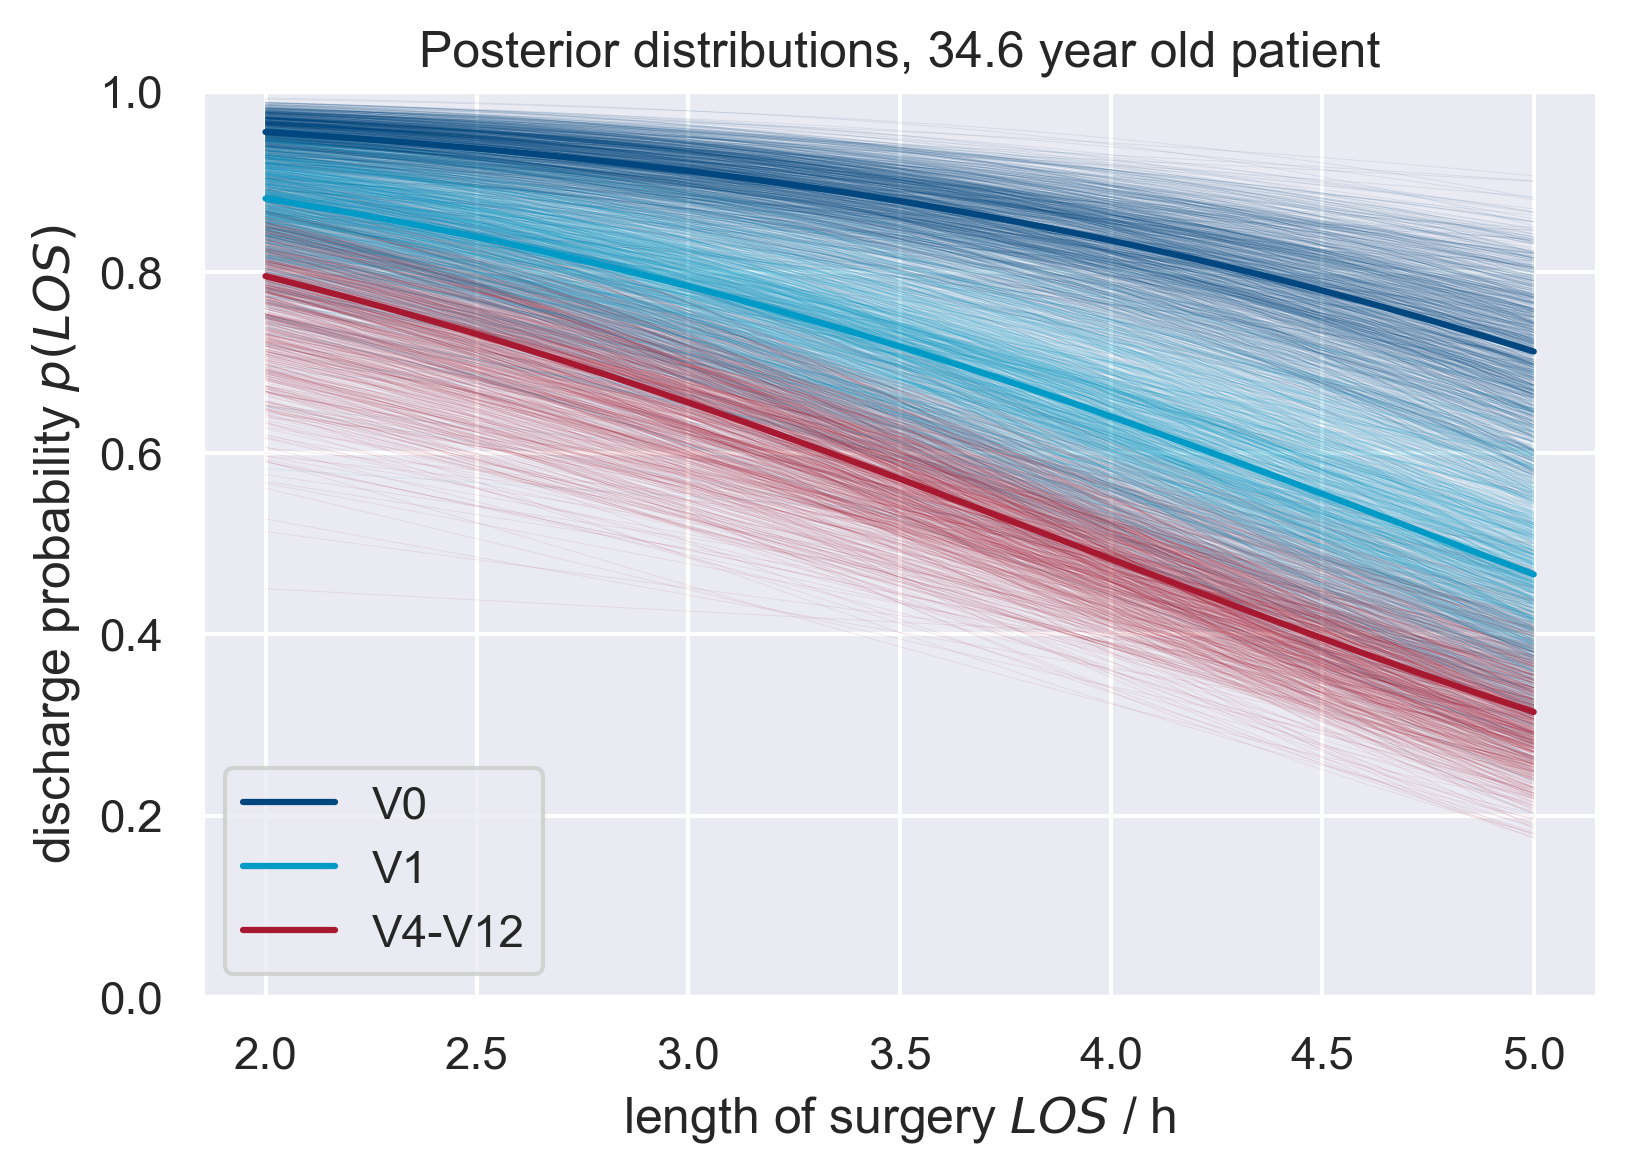
\includegraphics[width=0.5\textwidth]{images/DS19fk1_c0__p_LoS__model_B__traces_V0_V4-12__age_mean.png}&
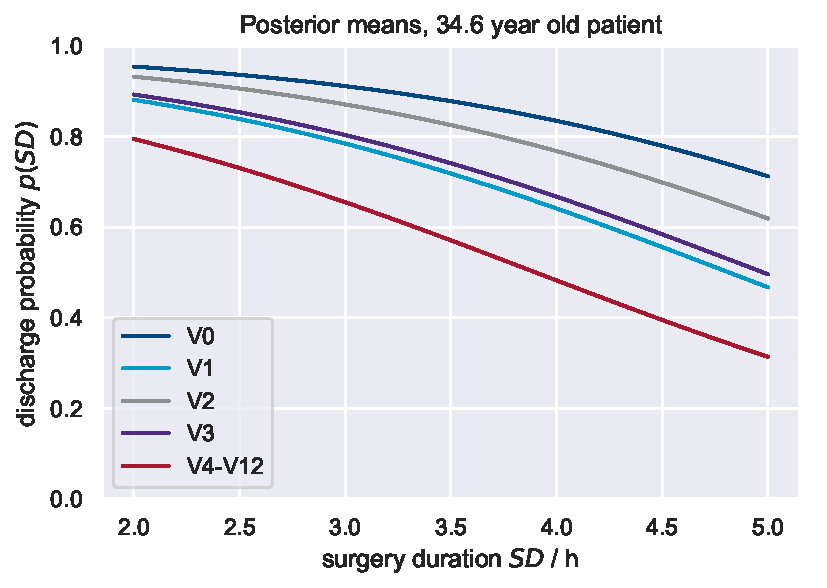
\includegraphics[width=0.5\textwidth]{images/DS19fk1_c0__p_LoS__model_B__mean__age_mean.pdf}\\
(c) & (d) \\
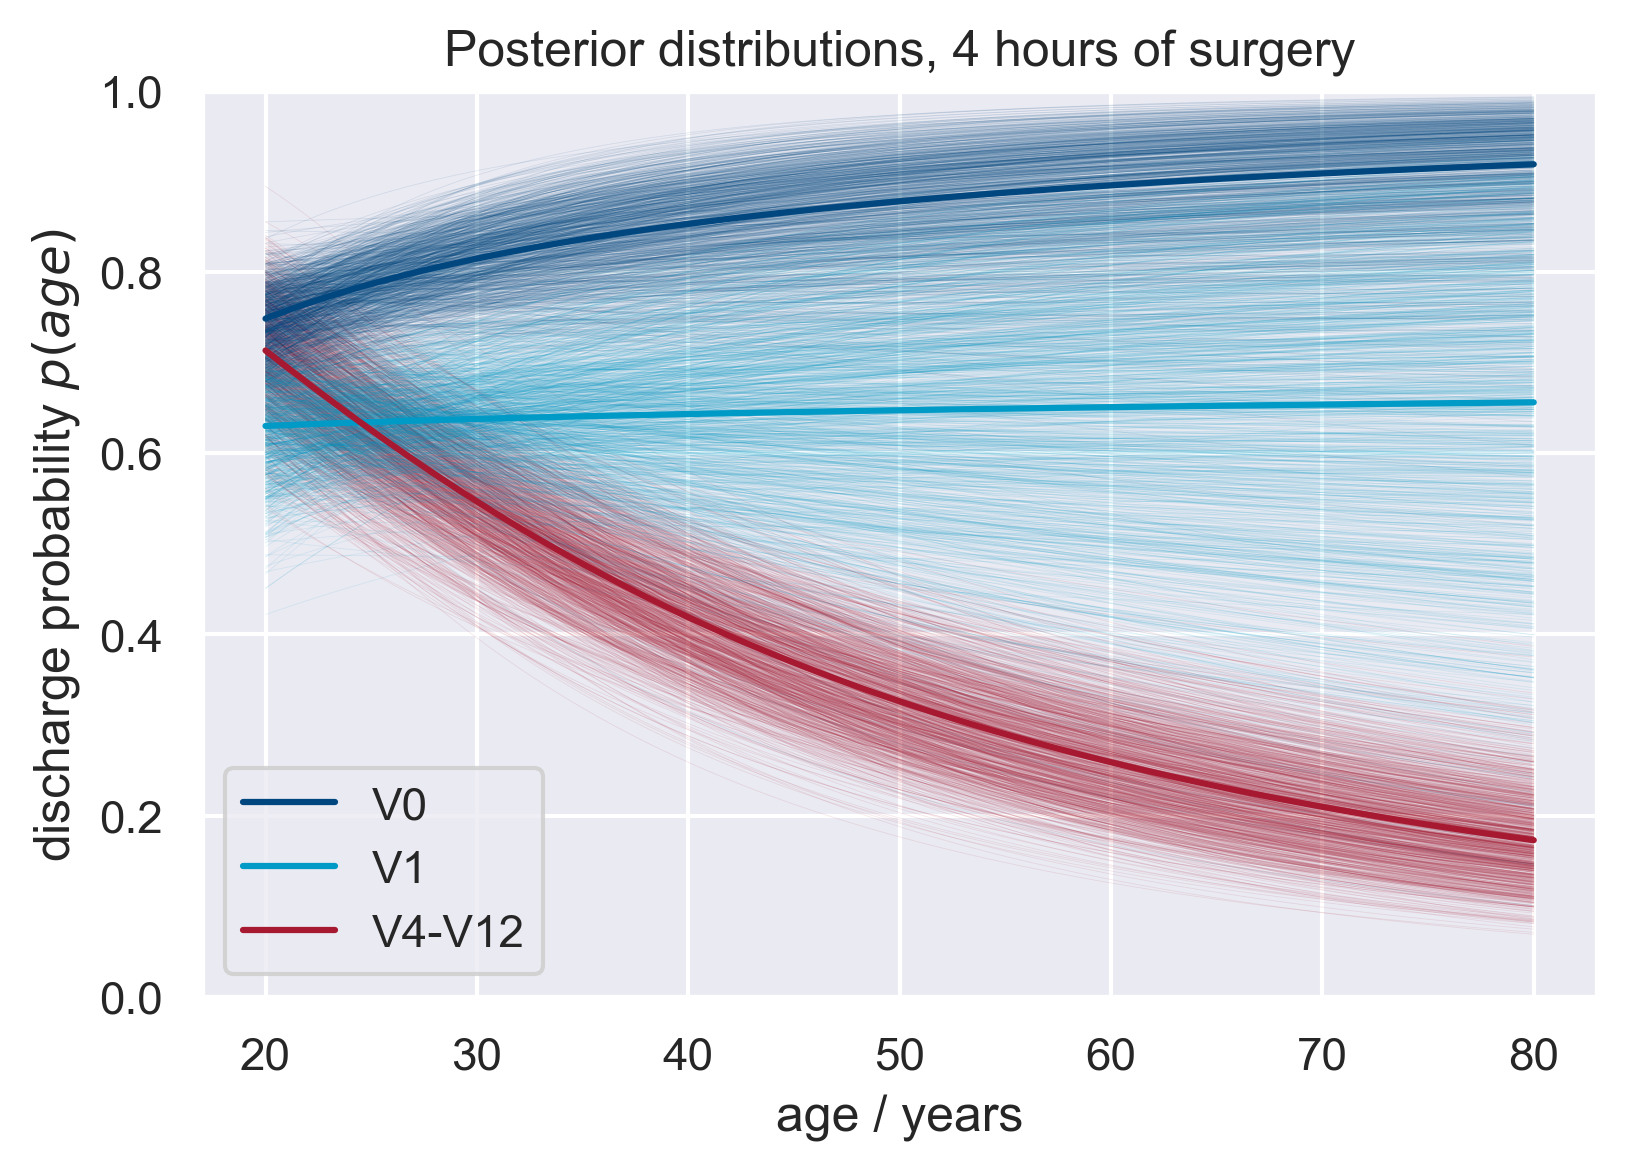
\includegraphics[width=0.5\textwidth]{images/DS19fk1_c0__p_age__model_B__traces__LoS_4h.png}&
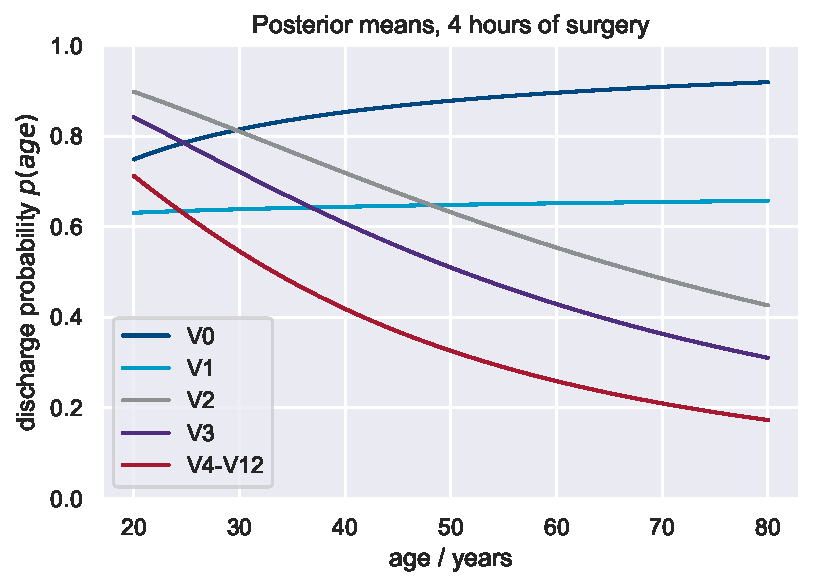
\includegraphics[width=0.5\textwidth]{images/DS19fk1_c0__p_age__model_B__mean__LoS_4h.pdf}\\
\end{tabular}
    \caption{Posterior distributions and corresponding means for
      different pathway variants of model B \eqref{modelB}. Trends with respect to
      SD and age are similar for model A \eqref{modelB}.}
    \label{fig:posterior}
\end{figure}

This is visualized in Fig.~\ref{fig:posterior}, which shows the posterior distributions of discharge probability $p_i$ as function of SD (Fig.~\ref{fig:posterior}(a)) and age (Fig.~\ref{fig:posterior}(c)). While the discharge probability decreases with increasing SD for all pathway variants (Fig.~\ref{fig:posterior}(b)), the effect is different for age. 
The discharge probability $p_i$ decreases for Variants V2, V3, and V4-V12 with increasing age of the patients, while its expectation value is constant for $V1$ and even increases by nearly 10\% for V0. Note, that the corresponding graphics for model A \eqref{modelA}, which are not shown here, resemble nearly the same correlations. 
From the clinical perspective, the difference in effects of age with
respect to the pathway variants might be related to the fact that the
most common pathway variants V0 and V1 are predominantly followed by younger patients (Fig.~\ref{Fig:boxplot}) and possibly older patients, for whom no complications are expected. 
However, the uncertainty of discharge probabilities for V1 is significantly larger compared to V0.

\begin{figure}
  \centering
  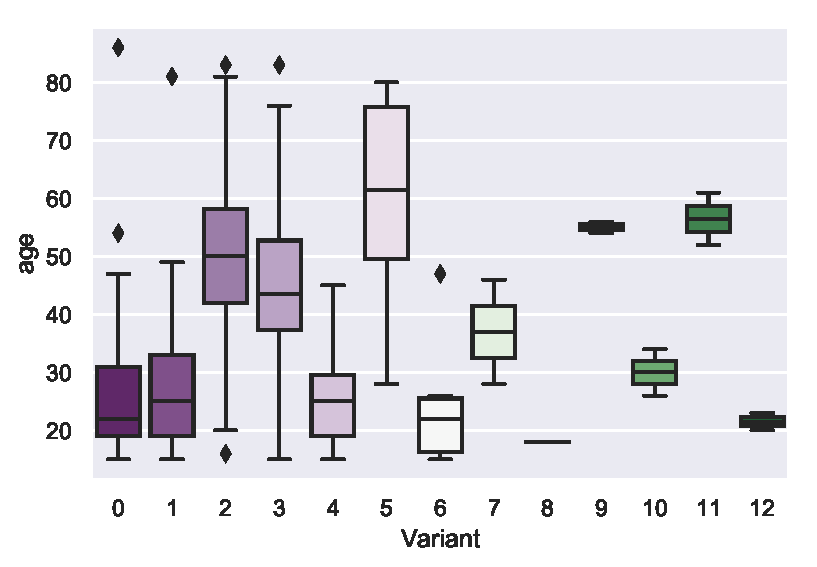
\includegraphics[width=0.618\textwidth]{images/DS19fA0_Lin20180730a__boxplot_age_variant.pdf}
\caption{Boxplot of patients' age for pathway variants of the
  appendicitis model.}
\label{Fig:boxplot}
\end{figure}
%\subsection{Cholecystitis Pathway Variants}
This section shows the cholecystitis pathway variant plot auto-generated by ProM. Cholecystitis pathway variants are analyzed without activities from the `antibiotics' sub-process and the `monitoring labs' sub-process (see section 3.7 for the activities from the two sub-processes). Clinicians confirmed that these sub-processes are standard monitoring and maintenance systems while the patient is waiting for further diagnosis. Only analyzing activities from the primary cholecystitis pathway significantly reduces the level of clinical variation between patient traces.

The cholecystitis pathway model consists of 10 pathway variants. The 10 pathway variants from the cholecystitis pathway model are shown in Fig.~\ref{fig:cholecystitis pathway variants}, and the number of patient traces that follow each pathway variant are listed in Table \ref{table:cholecystitis variant table}. Pathway variants from Fig.~\ref{fig:cholecystitis pathway variants} are ordered from the most frequent (index 0) to the least frequent (index 9). The most frequent pathway variant (index 0) consists of anesthesia, surgery, and surgical pathology lab. The second pathway variant (index 1) includes surgery without anesthesia because of faulty clinical data.

\begin{figure}[t]
\hspace{-2cm}
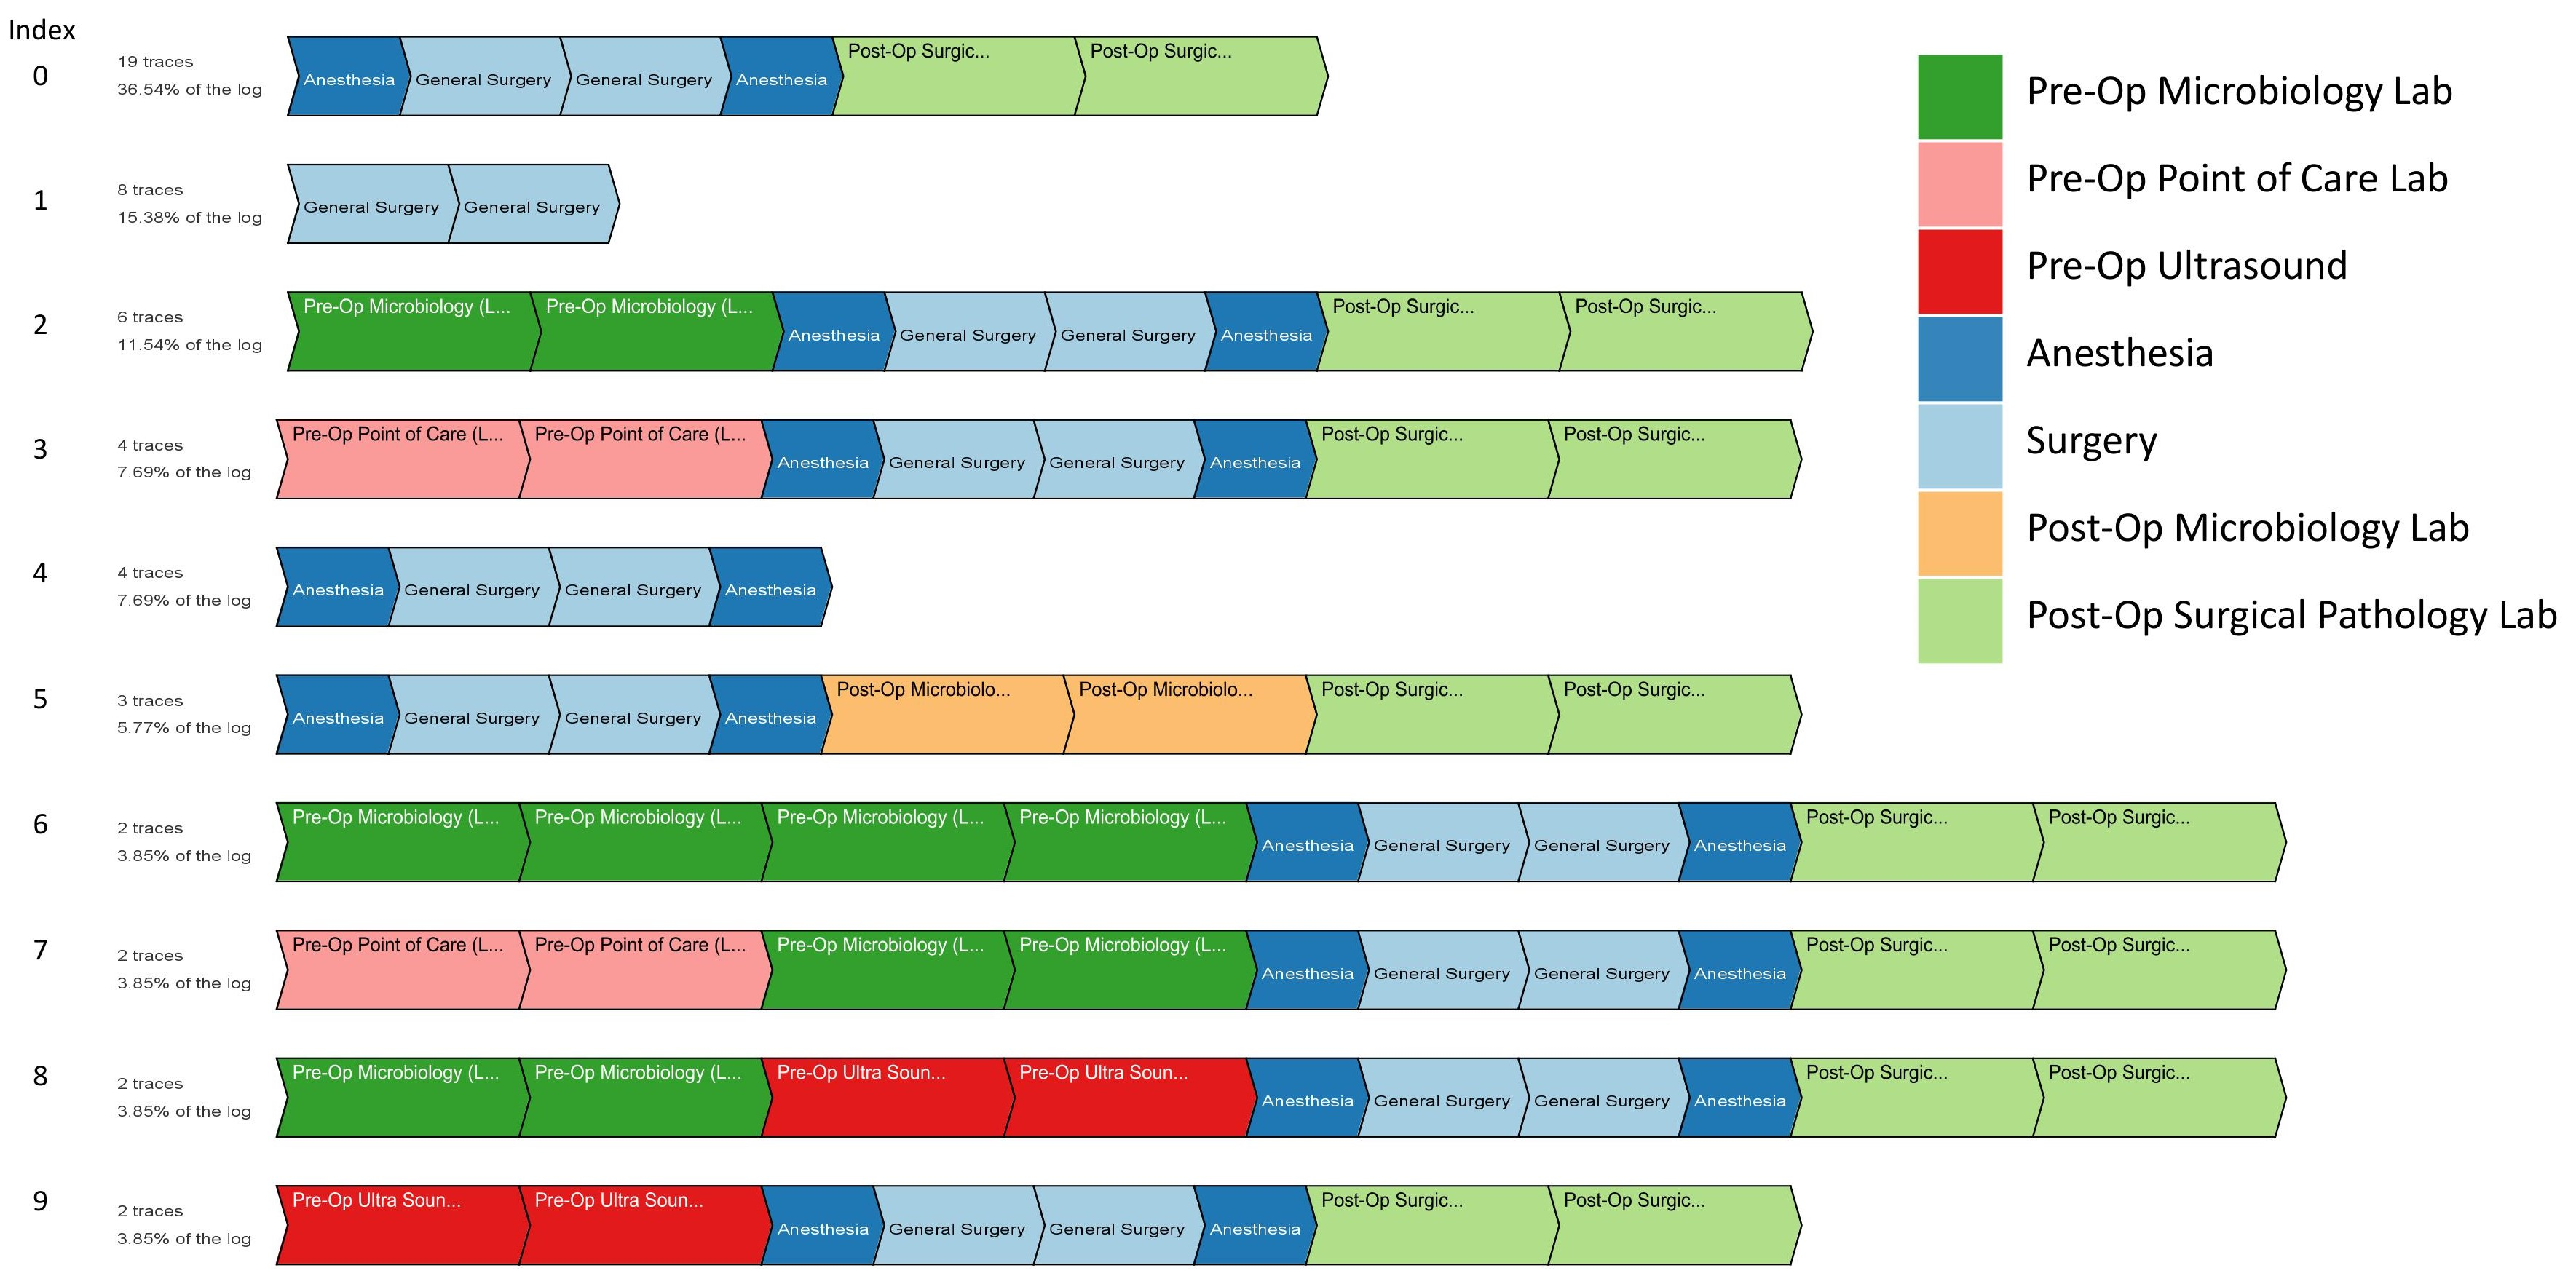
\includegraphics[width=1.5\textwidth]{images/cholecystitis_variant_index_anes.jpg}
\caption{Cholecystitis pathway variants auto-generated by ProM and appended with a legend. The top three pathway variants account for approximately 63\% of the patient traces. The statistics on the left are not readable in this reproduction but are listed in Table \ref{table:cholecystitis variant table}.}
\label{fig:cholecystitis pathway variants}
\end{figure}

\begin{table}[t]
\centering
\caption{Number of patient traces that follow each cholecystitis pathway variant.}
\label{table:cholecystitis variant table}
\begin{tabular}{ l l l }
 \hline
 Index & Number of Patient Traces & Percentage of Patients \% \\ 
 \hline
 0 & 19 & 36.54\\ 
 \hline
 1 & 8 & 15.38\\ 
 \hline
 2 & 6 & 11.54\\ 
 \hline
 3 & 4 & 7.69\\ 
 \hline
 4 & 4 & 7.69\\ 
 \hline
 5 & 3 & 5.77\\ 
 \hline
 6 & 2 & 3.85\\ 
 \hline
 7 & 2 & 3.85\\ 
 \hline
 8 & 2 & 3.85\\ 
 \hline
 9 & 2 & 3.85\\ 
 \hline
\end{tabular}
\end{table}

\subsection{Cholecystitis Pathway Model}
The cholecystitis pathway model visualized by \texttt{`Inductive Visual Miner'} incorporates activities from the `antibiotics' sub-process and the `monitoring labs' sub-process. A breakdown of the reformulated cholecystitis pathway model into one primary pathway and two concurrent sub-processes is shown in Fig.~\ref{fig:cholecystitis pathway model}, and the model notations are summarized in Table \ref{table:notation table}. The first pathway model in Fig.~\ref{fig:cholecystitis pathway model} is the primary pathway, followed by the `antibiotics’ sub-process and the `monitoring labs’ sub-process. Patient traces can execute any combination of the two sub-processes concurrently with the primary pathway. The eight patient traces that follow the second pathway variant (index 1) do not conform to this pathway model because of faulty clinical data. Based on this model, pre-operation haematology and chemistry labs tend to span the entire pre-operation process, while pre-operation antibiotics are taken closer to surgery.

\begin{figure}[t]
\centering
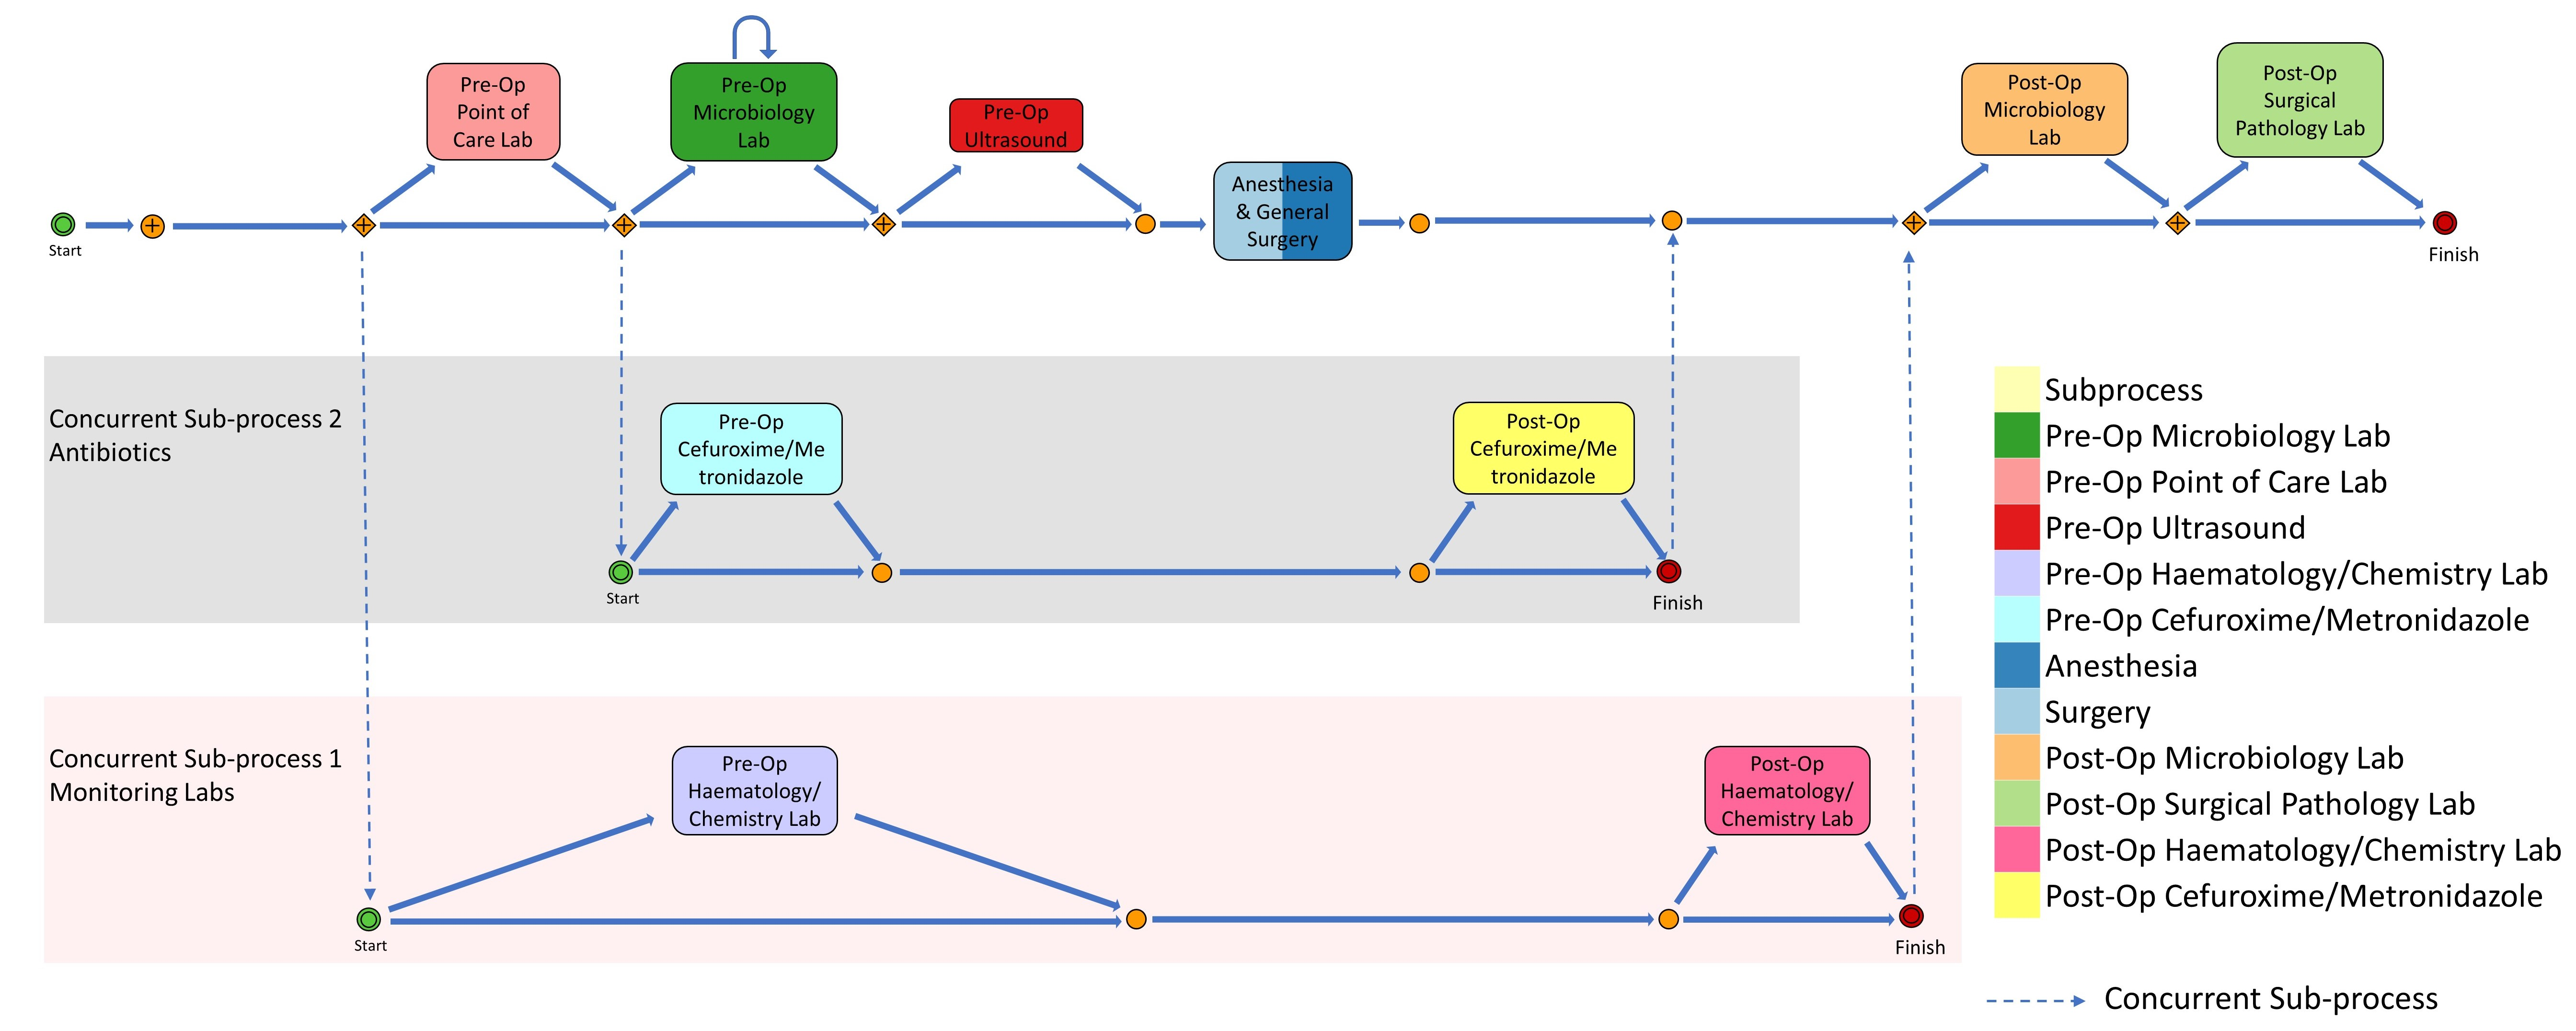
\includegraphics[width=18cm,angle=270]{images/communicative_cholecystitis_process_models_anes.jpg}
\caption{Cholecystitis pathway model. The model is broken down into one primary pathway and two sub-processes.}
\label{fig:cholecystitis pathway model}
\end{figure}

\section{Discussion from Thesis}
The aim of this study is to use business process modelling methods to design a process mining pipeline that supports discovery, conformance analysis, and enrichment of healthcare pathways from hospital health records, and to apply the designed pipeline to two clinical case studies. Results from the two case studies indicate that the designed pipeline with ProM as the main process mining tool is effective for mining both simple and complex healthcare pathway models to produce a concise form that is easy for clinical interpretation. This chapter discusses the advantages and limitations of the proposed healthcare pathway mining method for the three stages of analysis (i.e. healthcare pathway discovery, conformance, and enrichment). Future research directions that would maximize this study’s potential for industrial implementation are also discussed.

The discovery stage of the designed process mining pipeline provides an unbiased view of real patient experiences through the treatment process. The proposed approach to pathway discovery is data-based, so the accuracy of the output healthcare pathway model is highly dependent on data accuracy. Incorrectly logged health records in hospital information systems can lead to an inaccurate representation of real patient experiences through the treatment process, so clinicians must be consulted to determine if unexpected results are caused by faulty data. The main advantage of the proposed approach is that healthcare pathway visualization is automatic, and this means that the healthcare pathway mining pipeline has the potential to be fully automated in the future. Health records from the same hospital usually follow systematic formats and notations, so the process of converting electronic health records to clinical event logs compatible with business process mining software can be automated. The main challenge to automating the entire healthcare pathway discovery process is the event log processing steps required to reduce clinical variations. Even though the chapter on healthcare pathway mining methodology (Chapter 2) provides guidelines on processing steps that are effective for reducing unnecessary clinical variations in event logs, a certain level of clinical input is still required to ensure that no crucial information is filtered. In the first case study (see Chapter 3), appendicitis and cholecystitis pathways both contain repetitive activity patterns (i.e. antibiotics and monitoring labs) that result in incomprehensible spaghetti-models, and these patterns are identified by manual inspection of the pathway variants. There is potential for the process mining pipeline proposed in this study to be combined with clinical pattern mining algorithms developed in previous studies (e.g. the SCP-Miner and CCP-Miner developed by Huang, Lu, and Duan [16]) so that repetitive activity patterns can be identified and condensed automatically. Further research is required to determine the compatibility of the proposed process mining pipeline with various pattern mining algorithms.

The appendicitis and cholecystitis pathway models, from the first clinical case study, and the ambulatory cardiac care pathway model, from the second clinical case study, are all confirmed by clinicians to be easy to interpret and clinically meaningful, but one major limitation of the proposed pathway discovery approach is that the discovered healthcare pathway models can contain pathways that are not executed by any patient traces in the clinical event log. This is because the process mining software arranges all activities into a coherent pathway model by a configuration that summarizes all pathway variants, but a configuration that summarizes pathway variants does not guarantee that all pathways in the final healthcare pathway model make sense clinically. This also means that the pathway representation of models discovered by the proposed pipeline is unable to accurately capture all relations between activities. For example, the ambulatory cardiac care pathway model from the second case study (see Figure 56) shows that it is possible for patients to perform activity ‘Coronary Angiogram’ without performing ‘First Cardiology’ first. Close inspection of the event log revealed that patients who perform ‘Coronary Angiogram’ always perform ‘First Cardiology’ first, but this relation between the two activities is not evident in the discovered pathway model. Analysis of pathway variants instead of the pathway model does portray the true relations between all activities but this is not a realistic approach for complex healthcare pathways. For relatively simple healthcare pathways like the appendicitis and cholecystitis case study, patient traces can be organized into a manageable number of unique pathway variants and all variants can be analyzed individually. For complex healthcare pathways like the ambulatory cardiac care case study, patient traces cannot be organized into a manageable number of pathway variants because the level of variation between patients is too high. The healthcare pathway discovery stage of the methods presented here provides a concise overview of the fundamental structure of the overall pathway but does not always effectively capture the true relations between clinical activities. 
The conformance analysis stage of the designed process mining pipeline effectively identifies and visualizes patient deviations from the discovered healthcare pathway models. Even though this study only analyzes patient conformance to the discovered healthcare pathways, the same method could be applied analyze patient conformance to predefined ideal pathways or new pathway designs. The proposed approach to conformance analysis could be extended in the future to a monitoring tool to maintain quality of care for all patients. It is very difficult for clinicians to manually track individual patient traces through the treatment process and ensure that they are conforming to standard protocols. Identifying unwarranted deviations and making the required interventions early in the process has the potential to improve health outcomes and decrease cost. Even though the proposed approach effectively visualizes patient deviations, it cannot distinguish between clinically significant deviations and minor deviations that have no influence on patient health outcome. For example, some deviations are the results of scheduling availability and the order in which a required set of clinical activities are executed is not always relevant to health outcome. The proposed conformance analysis approach cannot automatically identify clinically significant deviations, and reasons for all deviations must be investigated manually. This is a major obstacle to future hospital implementation of the proposed pipeline, because it is inefficient and impractical to alert clinicians to minor patient deviations. Further research is required to develop a more specialized tool for conformance analysis that is able to classify patient deviations according to their association with patient health outcome.

The enrichment stage of the designed process mining pipeline is effective for identification of bottlenecks and treatment delays in healthcare pathways. The enrichment stage of the ambulatory cardiac care case study revealed that waiting times for transthoracic echo are exceedingly long (see §4.7), and resource reallocation is recommended to reduce the treatment delay. The effects of the delay on patient health outcome can be further investigated by computer simulations, but more clinical data is required for this approach. Analysis of waiting times and hospital length of stays is based on the assumption that the occurring timestamps of clinical activities are accurate. North Shore Hospital has an automated information system that stores patient records in real time and accuracy of the timestamps in the two case studies is therefore high, but the precision of activity timestamps is not always consistent across hospital systems. For example, one clinical department could record the exact time of day an activity is executed, while another department only records the date of execution. This leads to a margin of error of 24 hours, and this margin of error must be taken into account when interpreting the results. Accuracy and precision of clinical data must be assessed when the proposed pipeline is applied to new clinical case studies.

Analysis of pathway performance based on pathway variants reveals associations between clinical activities and performance indicators, but associations do not necessarily indicate causation. For example, the appendicitis pathway variants from the first case study that consist of postoperative imaging activities generally have longer postoperative length of stays, even though larger samples are required to confirm this connection (see §3.9). One possible explanation is that appendicitis patients that develop extra complications are more likely to require postoperative imaging activities. These are also the patients that remain under monitoring for a longer time period and hence have a delayed discharge date. Similarly, the ambulatory cardiac care pathway variants from the second case study that consist of visits to the emergency department generally have higher mortality rates (see §4.84.8). In both of these cases, patient condition is the main factor that influences the pathway performance indicators.
Dr. Andreas W. Kempa-Liehr’s work on developing probabilistic models to predict postoperative length of stay using information from the discovered healthcare pathway has the potential to improve the efficiency of hospital scheduling and resource allocation. This also shows that the proposed process mining pipeline has the potential to support the development of machine learning models for the prediction of performance indicators. A future improvement that could be made to the proposed pipeline is the incorporation of clinical diagnosis into the healthcare pathway models. Incorporating clinical diagnosis into pathway models allows for the identification of critical decision points where pathway variants diverge, but the main challenge is obtaining access to clinical diagnostic data. Overall, there is potential for the use of business process modelling techniques to improve the method of analysis of healthcare pathways, but the capability of other more specialized business process mining software should also be explored.

\section{Conclusion}
Healthcare pathways are critical for maintaining quality of care and
improving health outcome for all patients, but there is no consensus
on a healthcare pathway mining pipeline suitable for hospital
implementation that supports pathway discovery from hospital health
records.
Business process modelling methods are used to design a process mining
pipeline that produces concise and comprehensible healthcare pathway
models from hospital records, and supports conformance analysis and
enrichment of the discovered pathways.
The proposed process mining pipeline successfully constructs concise
pathway models for the appendicitis and cholecystitis case studies.
The produced healthcare pathway models are easy for clinical
interpretation and provide an unbiased overview of real patient traces
through the treatment process.
Probabilistic machine learning models for predicting postoperative
length of stay, using information extracted by the process mining
pipeline, is showing promising results.
This means that the proposed mining pipeline has the potential to
support the development of machine learning models to further relate
healthcare pathways to performance indicators.
This study has established the use of business process modelling methods for the improvement of healthcare pathway mining methods, and there is value in investigating the capabilities of other business process modelling tools for healthcare pathway mining purposes.

\begin{table}[h]
\centering
\begin{tabular}{p{11cm}} 
 Summary points\\ 
 What was already known:
 \begin{itemize}
     \item Healthcare pathways are critical for reducing clinical variability, affecting operational excellence, and thereby maximizing health outcomes.
     \item  Most healthcare pathways result from clinician-led practice rather than explicit pathway design via a consensus model and systems approach. 
     \item  There is currently no consensus on a systematic healthcare pathway mining method that supports explicit design and conformance analysis of concise and comprehensible healthcare pathway models.
 \end{itemize}
 What this study adds:
 \begin{itemize}
     \item  The use of business process modelling methods improves the automatic mapping of healthcare pathways from clinical data.
     \item The application of business process modelling methods to
       healthcare pathway enables deviations from typical treatment
       pathways to be identified, all using standard clinical data
       timestamps.
     \item Probabilistic machine learning models enable the prediction
       of patient specific discharge probabilities, which lead to
       patient specific postoperative
       length of stay distributions.
 \end{itemize}
\end{tabular}
\end{table}


\section*{Author Contributions}
\input{author_statement.txt}

\section*{Acknowledgements}
The authors like to thank Patrick Gladding for fruitful discussions.
This research has been funded by the Precision Driven Health research partnership (project number 1209).


\section*{Declaration of Competing Interests}
\input{conflict_of_interest.txt}

\bibliography{mybibfile}
%% Targeted for International Journal of Medical Informatics
% Word limit: 3000
%\documentclass[review]{elsarticle}
\documentclass{elsarticle}


\usepackage{lineno,hyperref,graphicx}
\usepackage{amsmath}
\usepackage[table]{xcolor}
\usepackage[section]{placeins}
\modulolinenumbers[5]
\graphicspath{ {./images/} }

% Adapted from https://www.overleaf.com/learn/how-to/Is_there_a_way_to_run_a_word_count_that_doesn%27t_include_LaTeX_commands%3F
\newcommand{\wordcount}[2]{%
  (\immediate\write18{texcount -1 -sum -merge #1.tex > #1-words.sum }%
  \input{#1-words.sum}/#2 words)%
}

\journal{Elsevier}

%%%%%%%%%%%%%%%%%%%%%%%
%% Elsevier bibliography styles
%%%%%%%%%%%%%%%%%%%%%%%
%% To change the style, put a % in front of the second line of the current style and
%% remove the % from the second line of the style you would like to use.
%%%%%%%%%%%%%%%%%%%%%%%

%% Numbered
%\bibliographystyle{model1-num-names}

%% Numbered without titles
%\bibliographystyle{model1a-num-names}

%% Harvard
%\bibliographystyle{model2-names.bst}\biboptions{authoryear}

%% Vancouver numbered
%\usepackage{numcompress}\bibliographystyle{model3-num-names}

%% Vancouver name/year
%\usepackage{numcompress}\bibliographystyle{model4-names}\biboptions{authoryear}

%% APA style
%\bibliographystyle{model5-names}\biboptions{authoryear}

%% AMA style
%\usepackage{numcompress}\bibliographystyle{model6-num-names}

%% `Elsevier LaTeX' style
\bibliographystyle{elsarticle-num}
%%%%%%%%%%%%%%%%%%%%%%%

\begin{document}
\newcommand{\plugin}[1]{\texttt{#1}}
\begin{frontmatter}

\title{Healthcare Pathway Discovery, Conformance, and Enrichment \wordcount{main-body}{3000}}

%% Group authors per affiliation:
%\author{Michael O’Sullivan,  Andreas W. Kempa-Liehr, Christina Lin\fnref{myfootnote}, Randall Britten, Delwyn Armstrong}
%\address{Radarweg 29, Amsterdam}
%\fntext[myfootnote]{Since 1880.}

%% or include affiliations in footnotes:
\author[mymainaddress]{Christina Lin\corref{mycorrespondingauthor}}
\cortext[mycorrespondingauthor]{Corresponding author}
\ead{clin364@aucklanduni.ac.nz}
\author[mymainaddress]{Andreas W. Kempa-Liehr}

\author[Orion]{Randall Britten}
\author[Waitemata]{Delwyn Armstrong}
\author[Waitemata]{Jonathan Wallace}
\author[Waitemata]{Patrick Gladding}
\author[mymainaddress]{ Michael O'Sullivan}

\address[mymainaddress]{Department of Engineering Science, The University of Auckland, 70 Symonds St, Auckland, New Zealand}
\address[Orion]{Orion Health, 181 Grafton Rd, Auckland, New Zealand}
\address[Waitemata]{Waitemata District Health Board, 124 Shakespeare Rd, Auckland, New Zealand
}

\begin{abstract}
\subsection*{Background and purpose}
Healthcare pathways define the execution sequence of clinical activities as patients move through a treatment process, and they are critical for maintaining quality of care. The aim of this study is to investigate the utilization of business process modelling (BPM) to design an adaptive healthcare pathway mining methodology, with particular emphasis on producing pathway models that are easy to interpret for clinicians without a sufficient background in process mining.

\subsection*{Method}
This study utilizes the business process-mining software ProM to design a process mining pipeline for healthcare pathway discovery, conformance analysis, and enrichment using hospital records. The efficacy of the BPM approach is demonstrated via two case studies that apply the proposed process mining pipeline to discover appendicitis and cholecystitis 
pathways from hospital records. Machine learning methodologies based on probabilistic programming are utilised to explore pathway features that influence patient recovery time.

\subsection*{Results}
The produced appendicitis and cholecystitis 
pathway models are
easy for clinical interpretation and provides an unbiased overview of patient movements through the treatment process. Analysis of the discovered pathway model enables reasons for longer than usual treatment times to be explored and deviations from standard treatment pathways to be identified. A probabilistic regression model that estimates patient recovery time based on the information extracted by the process mining pipeline is developed and has the potential to be very useful for hospital scheduling purposes.

\subsection*{Conclusion}
This study establishes the application of the business process modelling tool ProM for the improvement of healthcare pathway mining methods. 
%There is also value in investigating the capabilities of other business process modelling tools for healthcare pathway mining purposes. 
The proposed pipeline for healthcare pathway discovery  has the potential to support the development of machine learning models to further relate healthcare pathways to performance indicators such as length of post operation stay. 

\end{abstract}

\begin{keyword}
Healthcare pathway; Process mining; Electronic health record; Probabilistic programming
%\MSC[2010] 00-01\sep  99-00
\end{keyword}

\end{frontmatter}

\linenumbers

\section{Introduction}
Healthcare pathways are critical for reducing clinical variability, affecting operational excellence, and maximizing health outcomes \cite{Lin2001}. They define the execution sequence of clinical activities as patients move through a treatment process, a department, a hospital, or a wider health organization %(e.g., a District Health Board) 
\cite{Huang2016}. The accurate definition of healthcare pathways and patient conformance to those pathways is an issue of increasing relevance as precision medicine enables targeted approaches and diagnostic splitting. The proliferation of pathway branches is exponential, and pathways are increasingly non-linear. 

Most healthcare pathways result from clinician-led practice rather than explicit pathway design via a consensus model and systems approach. In addition, healthcare pathways “shift” dynamically as steps in the pathway are altered or resources change along the pathway. If no explicit redesign of pathways is performed, then the providers of the pathways (and its associated resources) may be unaware of the change \cite{Zhang2015}. Pathway discovery (identification of pathways without a priori knowledge), conformance analysis (including gaps in care and clinical variability) and pathway enrichment (enrichment of a priori models with additional event data) are critical for healthcare services now, and into the future \cite{Baker2017}.

Past studies have shown that there is potential for informative healthcare pathways to be extracted from hospital health records \cite{Xu2017}, \cite{Iwata2013}, but there is currently no consensus on a systematic healthcare pathway mining method that supports explicit design and conformance analysis of concise and comprehensible healthcare pathway models. The research described in this paper investigates the utilization of Business Process Modelling (BPM) as outlined by Becker et al. \cite{Becker2000} to provide a scaffold for healthcare pathway discovery, conformance analysis and enrichment. The main objectives of applying BPM to healthcare data include:
\begin{enumerate}
    \item Pathway discovery
    \begin{itemize}
        \item Investigate the potential of ProM (a process-mining software package) to discover healthcare pathways from hospital records \cite{VanDongen2005}.
    \end{itemize}
    \item Conformance analysis
    \begin{itemize}
        \item Apply BPM conformance analysis to discovered healthcare pathways. 
        \item Improve detection of possible non-conformance and explain anomalies.
    \end{itemize}
    \item Data enrichment
    \begin{itemize}
        \item Investigate correlation between healthcare pathway and performance indicators (e.g., patient length-of-stay, readmission rate).
    \end{itemize}
\end{enumerate}

\section{Healthcare Pathway Mining Methodology}
This section outlines the proposed process mining pipeline designed for mining healthcare pathways from hospital records using business process modelling tools. This study adopts the scientific computing practices recommended by Wilson et al. \cite{Wilson2014}, \cite{Wilson2017} to ensure that all results are reproducible. The proposed process mining pipeline consists of three major phases that correspond to each of the three main objectives (i.e. pathway discovery, conformance, and enrichment). An overview of the process mining pipeline designed for this study is shown in Fig.~\ref{fig:pipeline}.  The following sections elaborate the three phases of the proposed pipeline and their respective objectives.

\begin{figure}[t]
\centering
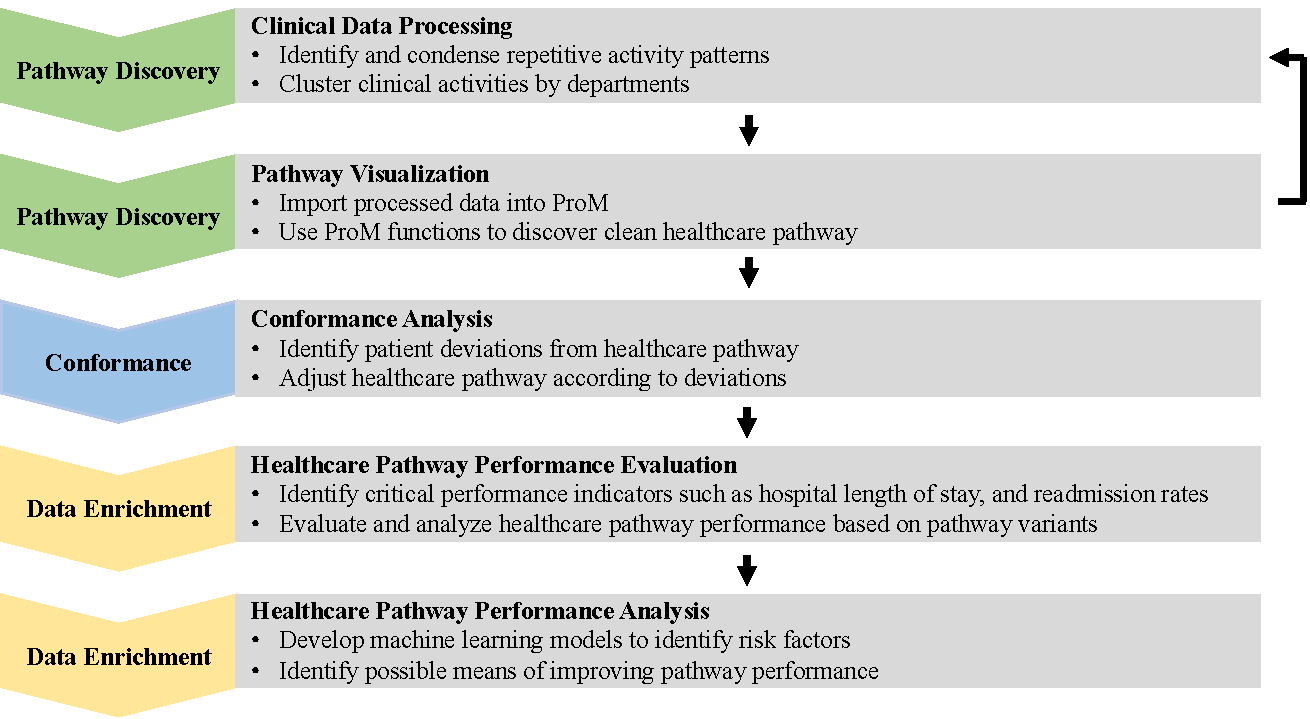
\includegraphics[width=\textwidth]{images/pipeline_diagram_journal.pdf}
\caption{The process mining pipeline comprises three sections, which
  are subdivided into five steps: Clinical data processing, pathway
  visualization, conformance analysis, healthcare pathway conformance
  evaluation, and prescriptive analytics of healthcare pathways. The
  first three steps are connected in two iterative cycles.}
\label{fig:pipeline}
\end{figure}

This study evaluates ProM (version 6.7) as the main process mining tool\footnote{\url{http://www.promtools.org}}. 
ProM is an open-source process mining software that is effective for construction of business models from input data files. ProM is chosen for this study because it has an intuitive user interface and supports many process mining plug-ins \cite{VanDongen2005}. The process mining and conformance analysis plug-ins supported by ProM are well documented. All these features of ProM make it easy for the process mining steps in the pipeline (see Fig.~\ref{fig:pipeline}) to be repeated by users with no background in process mining. The process mining techniques used in this paper are selected based on their ease for clinical interpretation and their potential to be combined with machine learning models. 

\subsection{Healthcare Pathway Discovery}
Healthcare pathway discovery is the first phase of the proposed process mining pipeline. It consists of two steps: clinical data processing and pathway visualization, which are conducted iteratively until a concise model is produced.
The aim is to use patient healthcare records stored in hospital information systems to design a concise pathway model that is easy for clinical interpretation. Therefore, clinical input is critical to the selection of appropriate processing methods. 
 
Healthcare pathways generally have much higher levels of complexity than standard business processes, and unprocessed clinical data contains too many clinical variations for a clean and concise pathway model to be mined \cite{Huang2013, Veiga2010}. Each pathway variant is a unique event sequence of a complete patient trace. The ProM plug-in \plugin{Explore Event Log} (from the Log Enhancement package) extracts pathway variants from patient traces, and the total number of pathway variants is an indicator of the level of clinical variation between patient traces. The basic format of an example pathway variant extracted by \plugin{Explore Event Log} is demonstrated in  Fig.~\ref{fig:example pathway variant}.

\begin{figure}[t]
\centering

\includegraphics[width=\textwidth]{images/example_pathway_variant_format2.jpg}
\caption{Basic format of example pathway variant visualized by ProM's
  plugin \plugin{Explore Event Log}. The same colour represents the same activity, and each activity is composed of a start event and a stop event.}
\label{fig:example pathway variant}
\end{figure}

In order to reduce healthcare pathway variations to a meaningful pathway model, the pathway variants visualized by the plug-in \plugin{Explore Event Log} are examined closely to determine the most suitable processing methods. 
There are three effective methods for reducing clinical variations without filtering patient traces:

\begin{description}
    \item[Cluster clinical activities] that are similar in nature so that the range of activities is reduced to a manageable size, e.g., `Abdomen CT scan' and `Pelvis CT scan' could be clustered into a single activity under `CT scan'.
    \item[Merge consecutive clinical activities] that are performed consecutively into a single activity, e.g., a patient receiving the same medication five times on the same day could be regarded as a single activity.
    \item[Condense repetitive activity patterns] 
         that repeat but exhibit variable cycle length. These patterns indicate an activity that must be performed periodically while the patient is waiting for a different activity to begin, e.g., lab tests to monitor a patient’s condition, medication to prevent infection. These repetitive patterns could be condensed into a single, parallel activity.
\end{description}
Clinical input is highly recommended at this step particularly for complex or unfamiliar healthcare pathways. 

%\subsubsection{Pathway Visualization}

\subsection{Healthcare Pathway Conformance Analysis}
It is very difficult for clinicians to manually track individual patient traces through the treatment process and ensure that they are conforming to standard protocols. Identifying unwarranted deviations and making the required interventions early in the process has the potential to improve health outcomes and decrease cost. 
Conformance analysis identifies patient deviations by comparing the pathway model to clinical data. 
Accuracy of the discovered healthcare pathway model is validated if the majority of the patient traces conform to the model. Patient traces rarely all follow identical pathways, so the healthcare pathway model is not expected to capture all patient traces. The objective is to discover a healthcare pathway model that captures the fundamental structure of most patient traces and detect unexpected patient deviations. 

ProM offers tools for conformance analysis of healthcare
pathway models: Its plug-in \plugin{Inductive Visual Miner} compares
patient traces from input clinical data to a healthcare pathway model
and indicates patient traces which are deviating from the pathway
model.
For this purpose, the pathway model is visualized as a process tree,
which is a hierarchical map comprised of decision nodes and
tasks representing clinical activities
\cite{25a7fd818bf44606a903d9b78b95cdd3}.
Therefore, process trees enable the identification of pathway branches
throughout the healthcare pathway model (c.f. Sec~\ref{Sec:AppendicitisDiscoveryConformance}).

If valid patient traces deviate from a healthcare pathway model, 
adjustments are made to the model to improve patient conformance.
A typical example might be the introduction of a new form of
treatment, which has not been included into the model yet.
Including these findings into the model leads to an iterative approach
between pathway discovery and conformance analysis (Fig.~\ref{fig:pipeline}).
Conversely, conformance analysis can identify where invalid
patient traces deviate from the model and investigate the reason for
the discrepancy, e.g., clinicians following obsolete pathways or data errors.

\subsection{Healthcare Pathway Data Enrichment}
% \subsubsection{Healthcare Pathway Performance Evaluation}
Data enrichment of healthcare pathways is the third phase of the
discussed process mining pipeline (Fig.~\ref{fig:pipeline}).
It comprises two steps: Healthcare pathway performance evaluation and
healthcare pathway performance analysis.

The main objectives of evaluating healthcare pathway performance are
to understand the strengths and weaknesses of the current pathway design,
and to identify potential methods of improvement. Possible indicators
of healthcare pathway performance include waiting times of clinical
activities, hospital length of stay, recovery time, and readmission
rates \cite{Rotter2008_pathways}.
Most of these indicators can be calculated or estimated using standard clinical timestamps. Postoperative Length of Stay (PLS), which is measured from leaving operating theatre to discharge, can also be considered as patient recovery time.
For surgical healthcare pathways,  PLS is one of the critical indicators for evaluating healthcare pathway
performance \cite{Pearson2001_pathways}. 

Analysing the performance of healthcare pathways with respect to
pathway variants and other possible influencing factors like
demographics or patient specific pathway characteristics, e.g. surgery duration (SD), is the final step of the process mining pipeline
(Fig.~\ref{fig:pipeline}).
Due to the fact, that most pathway performance indicators do not
follow normal distributions, while exhibiting significant stochastic
volatility, neither classical hypotheses tests \cite{Goodman2008_p-value}, nor point-predicting
machine learning models are appropriate for analysing healthcare
pathways.
Instead, probabilistic machine learning models
\cite{Ghahramani2015_PML} are used for extracting interpretable models
from healthcare pathways (Sec.~\ref{sec:ML}).
For this purpose, feature engineering \cite{DongLiu2018_FE} from
the patients' pathway traces (e.g. SD, pathway variant),
demographics (e.g. age), as well as medical documentation like written
diagnosis, time series, or images become important.
In order to demonstrate this approach, the following case study
discusses a probabilistic machine learning model for PLS, which
takes into account pathway variants
(Sec.~\ref{Sec:AppendicitisDiscoveryConformance}), as well as demographics, and
SD (Sec.~\ref{sec:ML}).

\section{Case Study: Appendicitis and Cholecystitis Healthcare Pathways}
This section discusses the healthcare pathway discovery process for the appendicitis and cholecystitis case studies. For this purpose, two years’ worth of data
from 2015 to 2017 on 448 appendicitis patients and 52 cholecystitis patients have been analysed. These case studies are selected because clinicians confirmed they are relatively simple surgical pathways with clear start and end points.

\subsection{Data Description}
\label{Sec:DataDescription}
The patient records for both case studies were collected from North Shore Hospital in Auckland, New Zealand.
The data were de-identified and an ethics approval for this research was obtained. All data sets collected from the hospital's information system on appendicitis and cholecystitis patients are summarized in Tab.~\ref{table:data description table}. Theatre encounter is the system ID used to identify patient traces, and clinical activities are categorized by clinical departments (e.g. radiology, pharmacy). Unfortunately, patient demographics data is only available for appendicitis patients. These data sets are processed and imported into ProM for pathway discovery and conformance analysis.

\newcommand{\tabitem}{~~\llap{\textbullet}~~}

\begin{table}[t]
\centering
\caption{Description of all data sets collected from North Shore Hospital for the appendicitis and cholecystitis case studies.}
\label{table:data description table}
\begin{tabular}{lll}
  \hline
  \hline
EMR  &     Columns of Interest & Data Type  \\
\hline
Acute Theatre   &    \tabitem Theatre Encounter & String\\  &\tabitem Surgery Start Time & Datetime\\  &\tabitem Surgery End Time & Datetime\\  &\tabitem Into Theatre Time & Datetime\\  &\tabitem Out of Theatre Time & Datetime\\
  \hline
General Surgery   &    \tabitem Theatre Encounter & String\\  &\tabitem Admission Time & Datetime\\  &\tabitem Discharge Time & Datetime\\
  \hline
Radiology/Pharmacy   &    \tabitem Theatre Encounter & String\\  /Lab/Anesthesia & \tabitem Clinical Activity & String\\  &\tabitem Clinical Activity Start Time  & Datetime\\
  \hline
Patient    &    \tabitem Theatre Encounter & String\\(specific to appendicitis patients)  &\tabitem Patient Age & Integer\\  &\tabitem Patient Gender  & String\\  &\tabitem Patient Ethnicity  & String\\
  \hline
  \hline
\end{tabular}
\end{table}

\subsection{Appendicitis Pathway Discovery and Conformance Analysis}
\label{Sec:AppendicitisDiscoveryConformance}
The appendicitis pathway model, which has been generated by ProM's
plugin \plugin{Explore Event Log}, is shown in
Fig.~\ref{fig:appendicitis pathway variants} in the form of a pathway
variant plot.
The pathway variants are extracted without activities related to medication (i.e. preoperative and postoperative cefuroxime/metronidazole) because the clinicians confirmed that antibiotics are usually taken while the patient is waiting for surgery or discharge. The duration of these activities are therefore highly variable and result in a high number of unique pathway variants.

%The variant specific numbers of patient traces given in  Fig.~\ref{fig:appendicitis pathway variants} are repeated in Tab.~\ref{table:appendicitis variant table}.
The pathway variant plot visualizes the 13 pathway variants of the
appendicitis model sorted from the most common pathway (index 0) to
the least common pathway (index 12).
The top four variants account for approximately 88\% of the patient
traces (Tab.~\ref{table:appendicitis variant table}).
All clinical activities are represented by a start event and a stop
event.
The activities are colour coded such that the same colour refers to the same clinical activity. The most common pathway variant (index 0) only consists of anesthesia and surgery, while the second most common variant (index 1) also includes preoperative X-ray.
The pathway variant indices are used in Sec.~\ref{sec:ML} as one-hot
encoded feature of the probabilistic machine learning model.

\begin{figure}[t]
\hspace{-2cm}
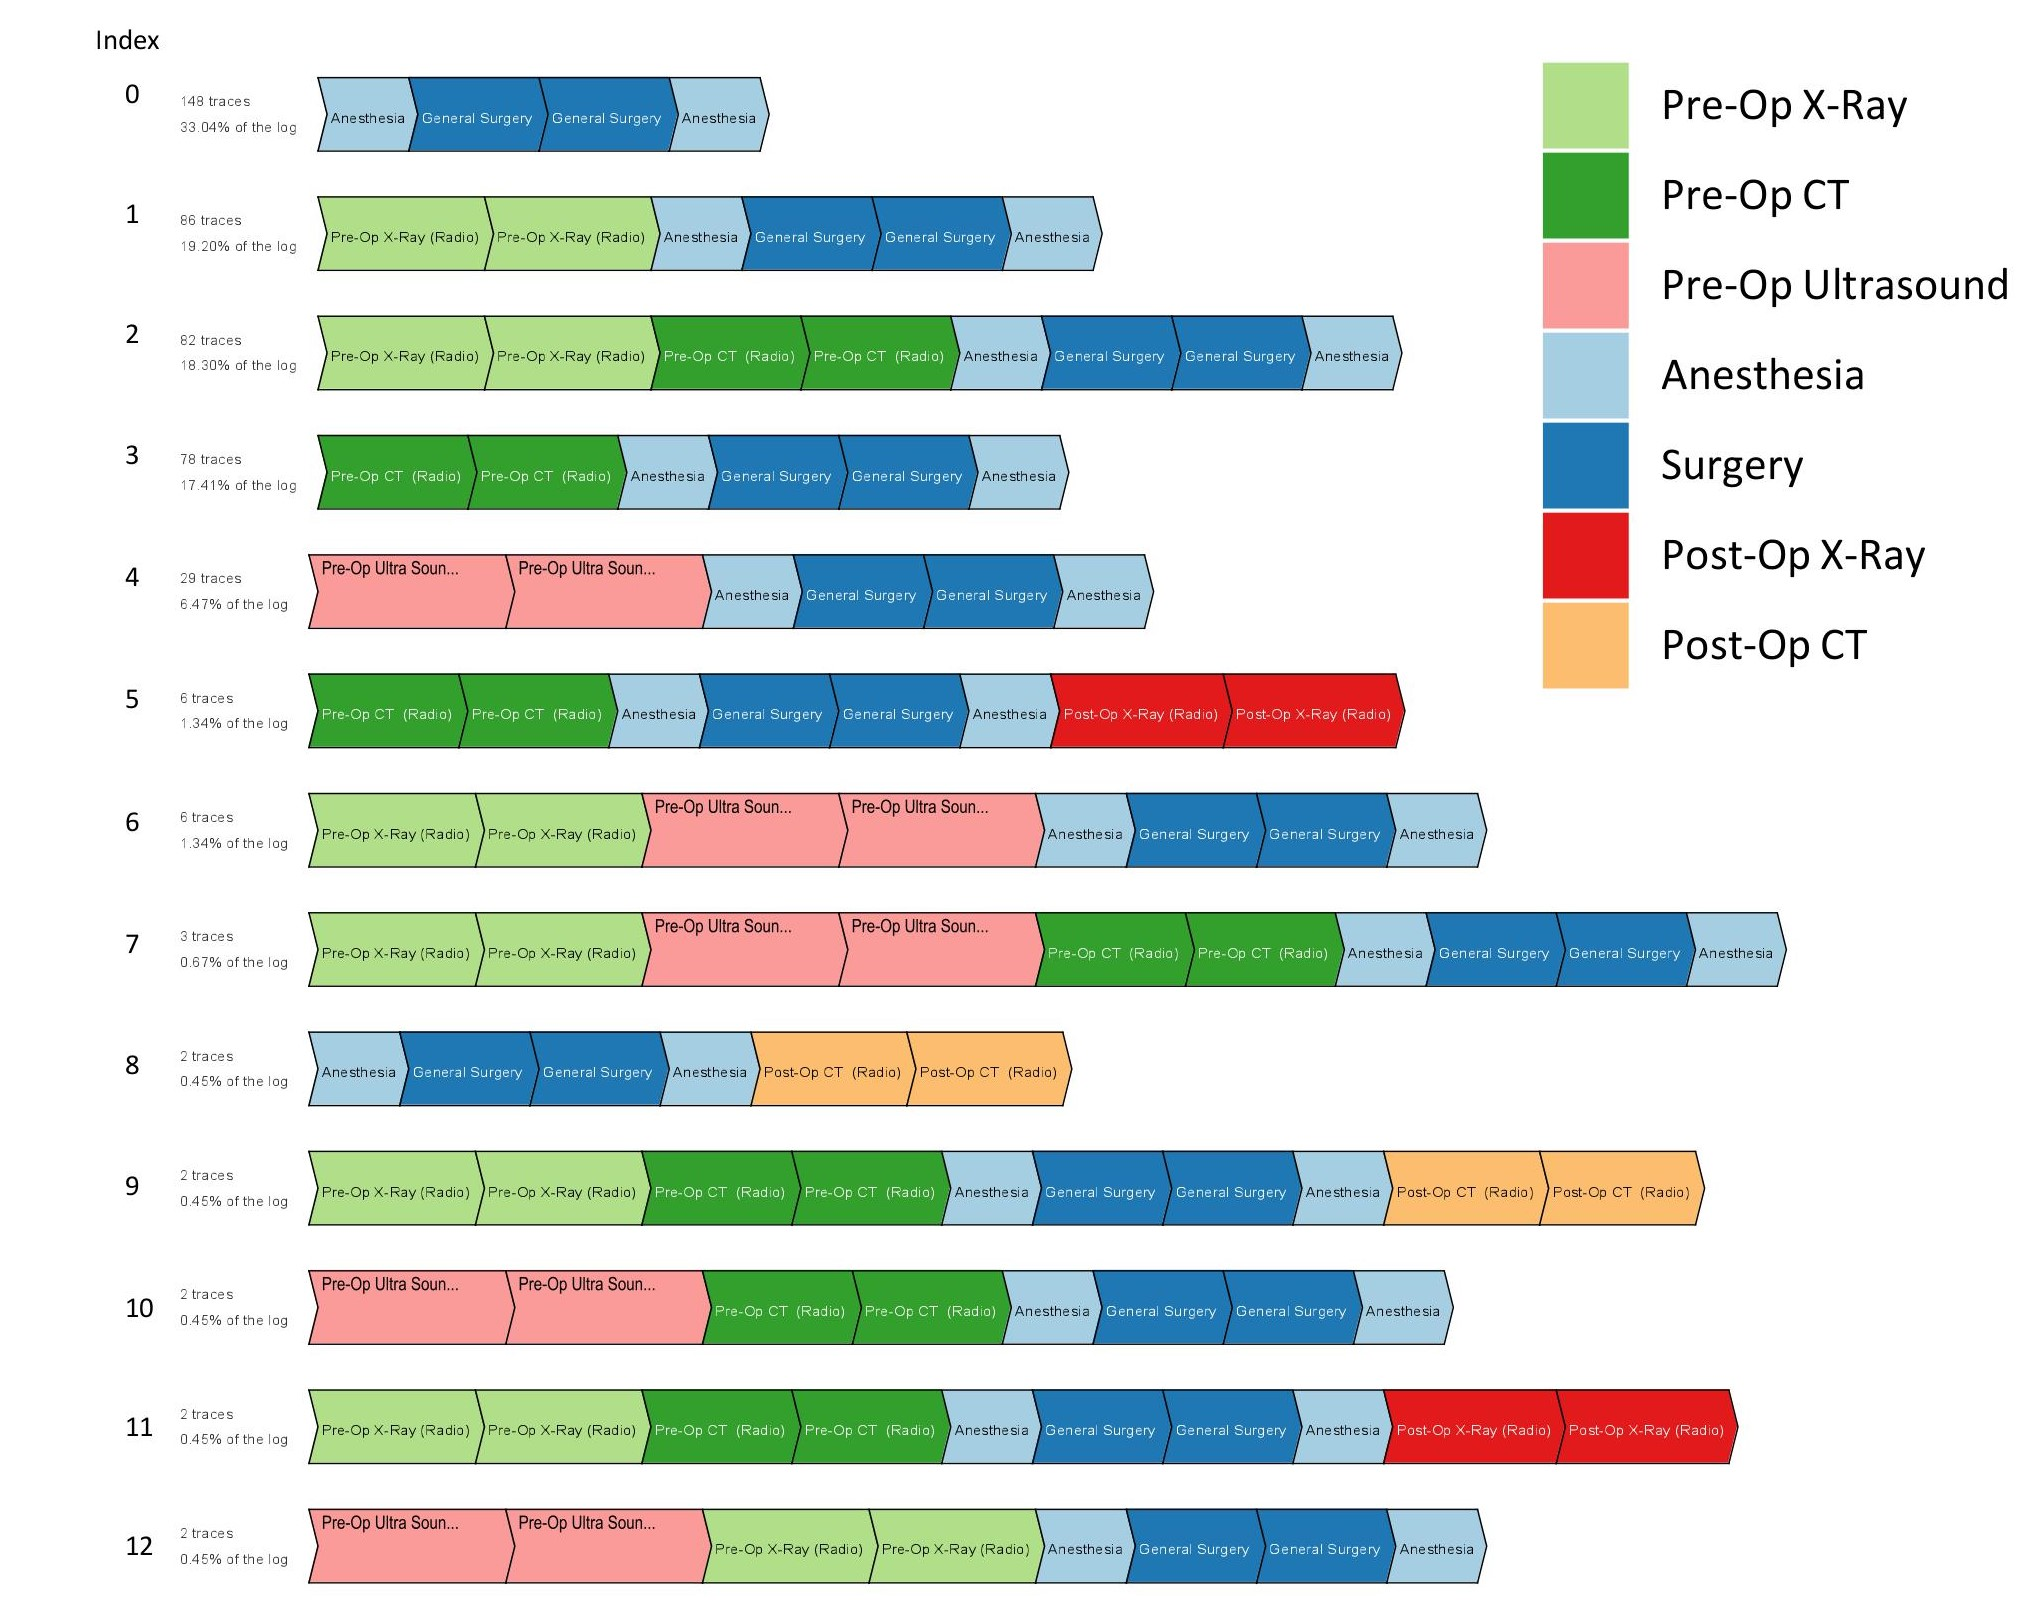
\includegraphics[width=1.5\textwidth]{images/appendicitis_variant_index_anes.jpg}
\caption{Appendicitis pathway variant plot auto-generated by ProM's
  plugin \plugin{Explore Event Log}. 
  The plot visualizes the sequences of start and stop events for the different pathways.
  For the purpose of readability the legend was added and the
  statistics on the left are repeated in Tab.~\ref{table:appendicitis variant table}.
 The top four variants account for approximately 88\% of the patient
 traces. They are modelled as one-hot encoded features V0, V1, V2, and V3
 in Sec.~\ref{sec:ML}, while pathway variants V4--V12 together represent
 the base model.
 }
\label{fig:appendicitis pathway variants}
\end{figure}
\clearpage

\begin{table}[t]
\centering
\caption{Statistics of appendicitis patient traces shown in Fig.~\ref{fig:appendicitis pathway variants}.}
\label{table:appendicitis variant table}
\begin{tabular}{llllllll}
  \hline
  \hline
Variant &     0  &     1  &     2  &     3  &    4  &    5  &    6  \\
\hline
Patients   &    148 &     86 &     82 &     78 &    29 &     6 &     6 \\
  Percentage &  33.04\% &  19.20\% &  18.30\% &  17.41\% &  6.47\% &  1.34\% &  1.34\%\\
  \hline
  \hline
Variant &     7  &    8  &    9  &    10 &    11 &    12 \\
\hline
Patients   &   3 &     2 &     2 &     2 &     2 &     2 \\
Percentage &  0.67\% &  0.45\% &  0.45\% &  0.45\% &  0.45\% &  0.45\% \\
  \hline
  \hline
\end{tabular}
\end{table}

The first stage of the appendicitis pathway model visualized by \plugin{Inductive Visual Miner} is shown in Fig.~\ref{fig:ivm pathway model example}.
Unlike the pathway variants, this appendicitis pathway model incorporates activities representing antibiotics. The model indicates that 42 patients perform ultrasound and 183 patients perform X-ray upon admission. 

\begin{figure}[t]
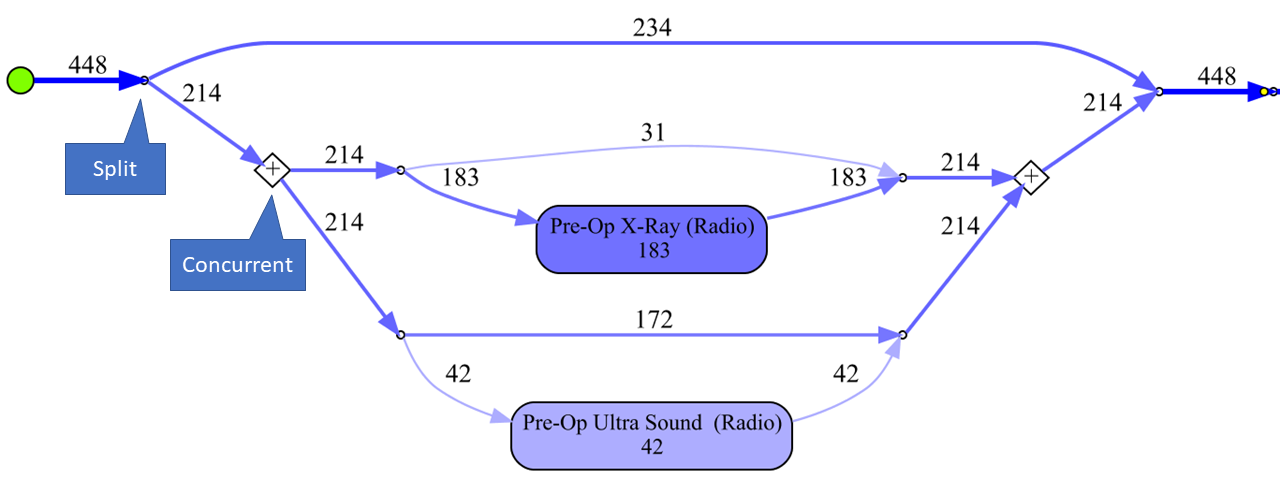
\includegraphics[width=\textwidth]{images/ivm_appendicitis_first_stage_example.png}
\caption{First stage of the appendicitis pathway model generated by
  ProM. The following stages have been omitted for the purpose of
  readability.
  The process indicates that 234 patients do not have any preoperative
  imaging diagnostics, while 214 patients enter the imaging
  diagnostics branch.
  Please refer to Leeman's manual on \plugin{Inductive Visual Miner} for details on the model notations \cite{leemansinductive}.}
\label{fig:ivm pathway model example}

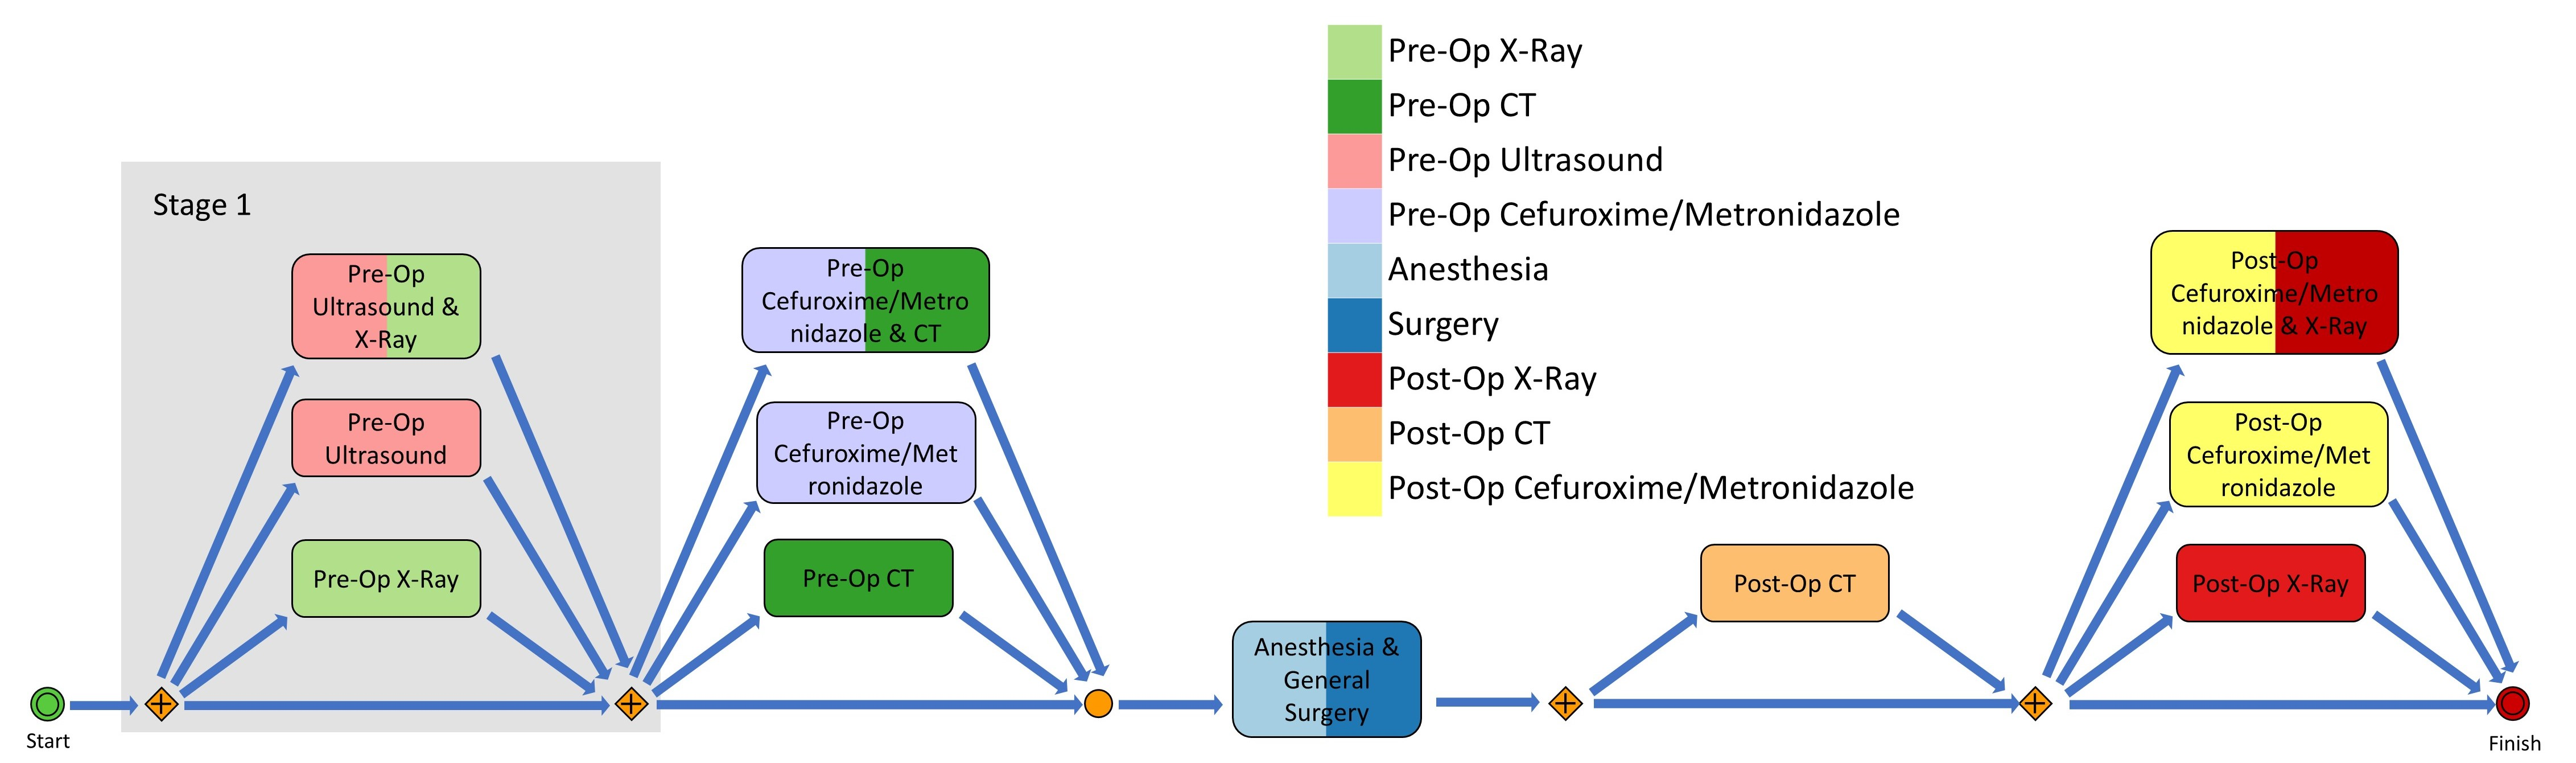
\includegraphics[width=\textwidth]{images/communicative_appendicitis_process_models_anes.jpg}
\caption{Appendicitis pathway model using nomenclature of Tab.~\ref{table:notation table}. All preoperative and
  postoperative activities belong to radiology and pharmacy
  departments. Preoperative antibiotics are taken in the second stage
  of the treatment pathway.}
\label{fig:appendicitis pathway model}
\end{figure}

While the complex process tree notation of ProM's \plugin{Inductive
  Visual Miner} plugin is optimal for detailed analysis, it has been
reformulated under new notations for easy clinical interpretation.
The new model notations are summarized in Table \ref{table:notation
  table}, and the reformulated appendicitis pathway model is shown in
Fig.~\ref{fig:appendicitis pathway model}. The section of the model
labelled as `Stage 1' in Fig.~\ref{fig:appendicitis pathway model}
corresponds to the process tree shown in Fig.~\ref{fig:ivm pathway
  model example}.
This is the final pathway model that has been compiled based on
clinical input to account for valid patient deviations, and all
patient traces conform to the updated pathway.
The most common pathway variant (index 0) shown in Fig.~\ref{fig:appendicitis pathway variants} corresponds to the horizontal path from start to finish in Fig.~\ref{fig:appendicitis pathway model}.

\begin{table}[t]
\centering
\caption{Definitions of new pathway model notations.}
\label{table:notation table}
\begin{tabular}{ l c l }
 \hline
 \hline
 Notation & Symbol & Definition \\ 
 \hline
 Orange Diamond 
 &
%\raisebox{-\totalheight}{\includegraphics[width=0.3\textwidth, height=60mm]{images/myLboro.png}}
 \raisebox{-3pt}{
\includegraphics[width=0.5cm]{images/decision_node.png}}
 & Decision Point, indicating exclusive choice \\ 
 \hline
 Orange Connector 
 & 
 \raisebox{-3pt}{
\includegraphics[width=0.5cm]{images/connection_node.png}}
 & Pathway Connection Point \\
 \hline
 Green Connector 
 & 
 \raisebox{-3pt}{
\includegraphics[width=0.5cm]{images/start_node.png}}
 & Starting Point \\
 \hline
 Red Connector 
 & 
 \raisebox{-3pt}{
\includegraphics[width=0.5cm]{images/finish_node.png}} 
 & Finishing Point \\
 \hline
 \hline
\end{tabular}
\end{table}

\subsection{Length of Stays of Appendicitis Pathway Variants}
Length of stays in hospital are analyzed based on the 13 identified appendicitis pathway variants shown in Fig.~\ref{fig:appendicitis pathway variants}. Hospital length of stay, measured from admission to discharge, for each of the 13 appendicitis pathway variants are shown in Fig.~\ref{fig:hospital length of stay appendicitis}. Postoperative length of stay, measured from leaving theatre to discharge, for each pathway variant is shown in Fig.~\ref{fig:post op length of stay appendicitis}. Pathway variant 9 has the longest length of stay for both measures. Pathway variants 5, 7 and 11 also have relatively long length of stays. Out of these four pathway variants, only pathway variant 7 consists of no postoperative activities. The number of patient traces that follow each pathway variant is limited, and more samples are required to identify rate-determining steps. Probabilistic machine learning models are used to further investigate factors influencing postoperative length of stay (Sec.~\ref{sec:ML}).

\begin{figure}[t]
\centering
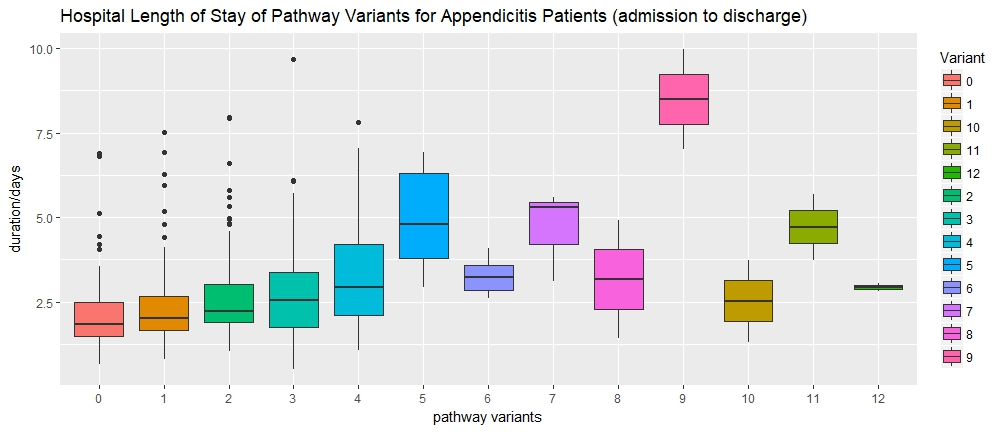
\includegraphics[width=\textwidth]{images/hospital_length_of_stay_appendicitis_210518.jpeg}
\caption{Hospital length of stay of the 13 appendicitis pathway variants, measured from admission to discharge.}
\label{fig:hospital length of stay appendicitis}
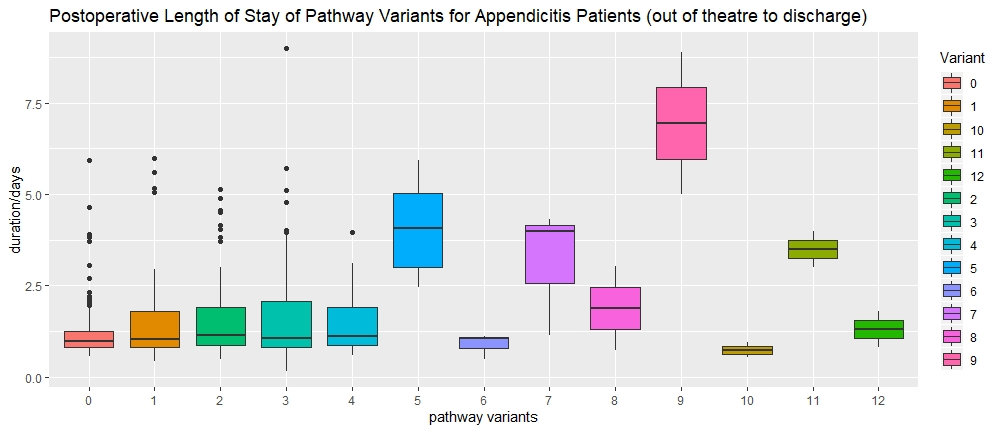
\includegraphics[width=\textwidth]{images/postoperative_length_of_stay_appendicitis.jpeg}
\caption{Postoperative length of stay of the 13 appendicitis pathway variants, measured from leaving theatre to discharge.}
\label{fig:post op length of stay appendicitis}
\end{figure}

\subsection{Cholecystitis Pathway Discovery and Conformance Analysis}
\label{Sec:CholecystitisDiscoveryConformance}
This section shows the cholecystitis pathway variant plot auto-generated by ProM. Cholecystitis pathway variants are analyzed without activities from the `antibiotics' sub-process and the `monitoring labs' sub-process (see Fig.~\ref{fig:cholecystitis pathway model} for the activities from the two sub-processes). Clinicians confirmed that these sub-processes are standard monitoring and maintenance systems while the patient is waiting for further diagnosis. Only analyzing activities from the primary cholecystitis pathway significantly reduces the level of clinical variation between patient traces.

The cholecystitis pathway model consists of 10 pathway variants. The 10 pathway variants of the cholecystitis pathway model are shown in Fig.~\ref{fig:cholecystitis pathway variants}, and the number of patient traces that follow each pathway variant are listed in Table \ref{table:cholecystitis variant table}. Pathway variants from Fig.~\ref{fig:cholecystitis pathway variants} are sorted from the most common pathway (index 0) to the least common pathway (index 9). The most common pathway variant (index 0) consists of anesthesia, surgery, and surgical pathology lab. The second pathway variant (index 1) includes surgery without anesthesia because of faulty clinical data. 

\begin{figure}[t]
\hspace{-2cm}
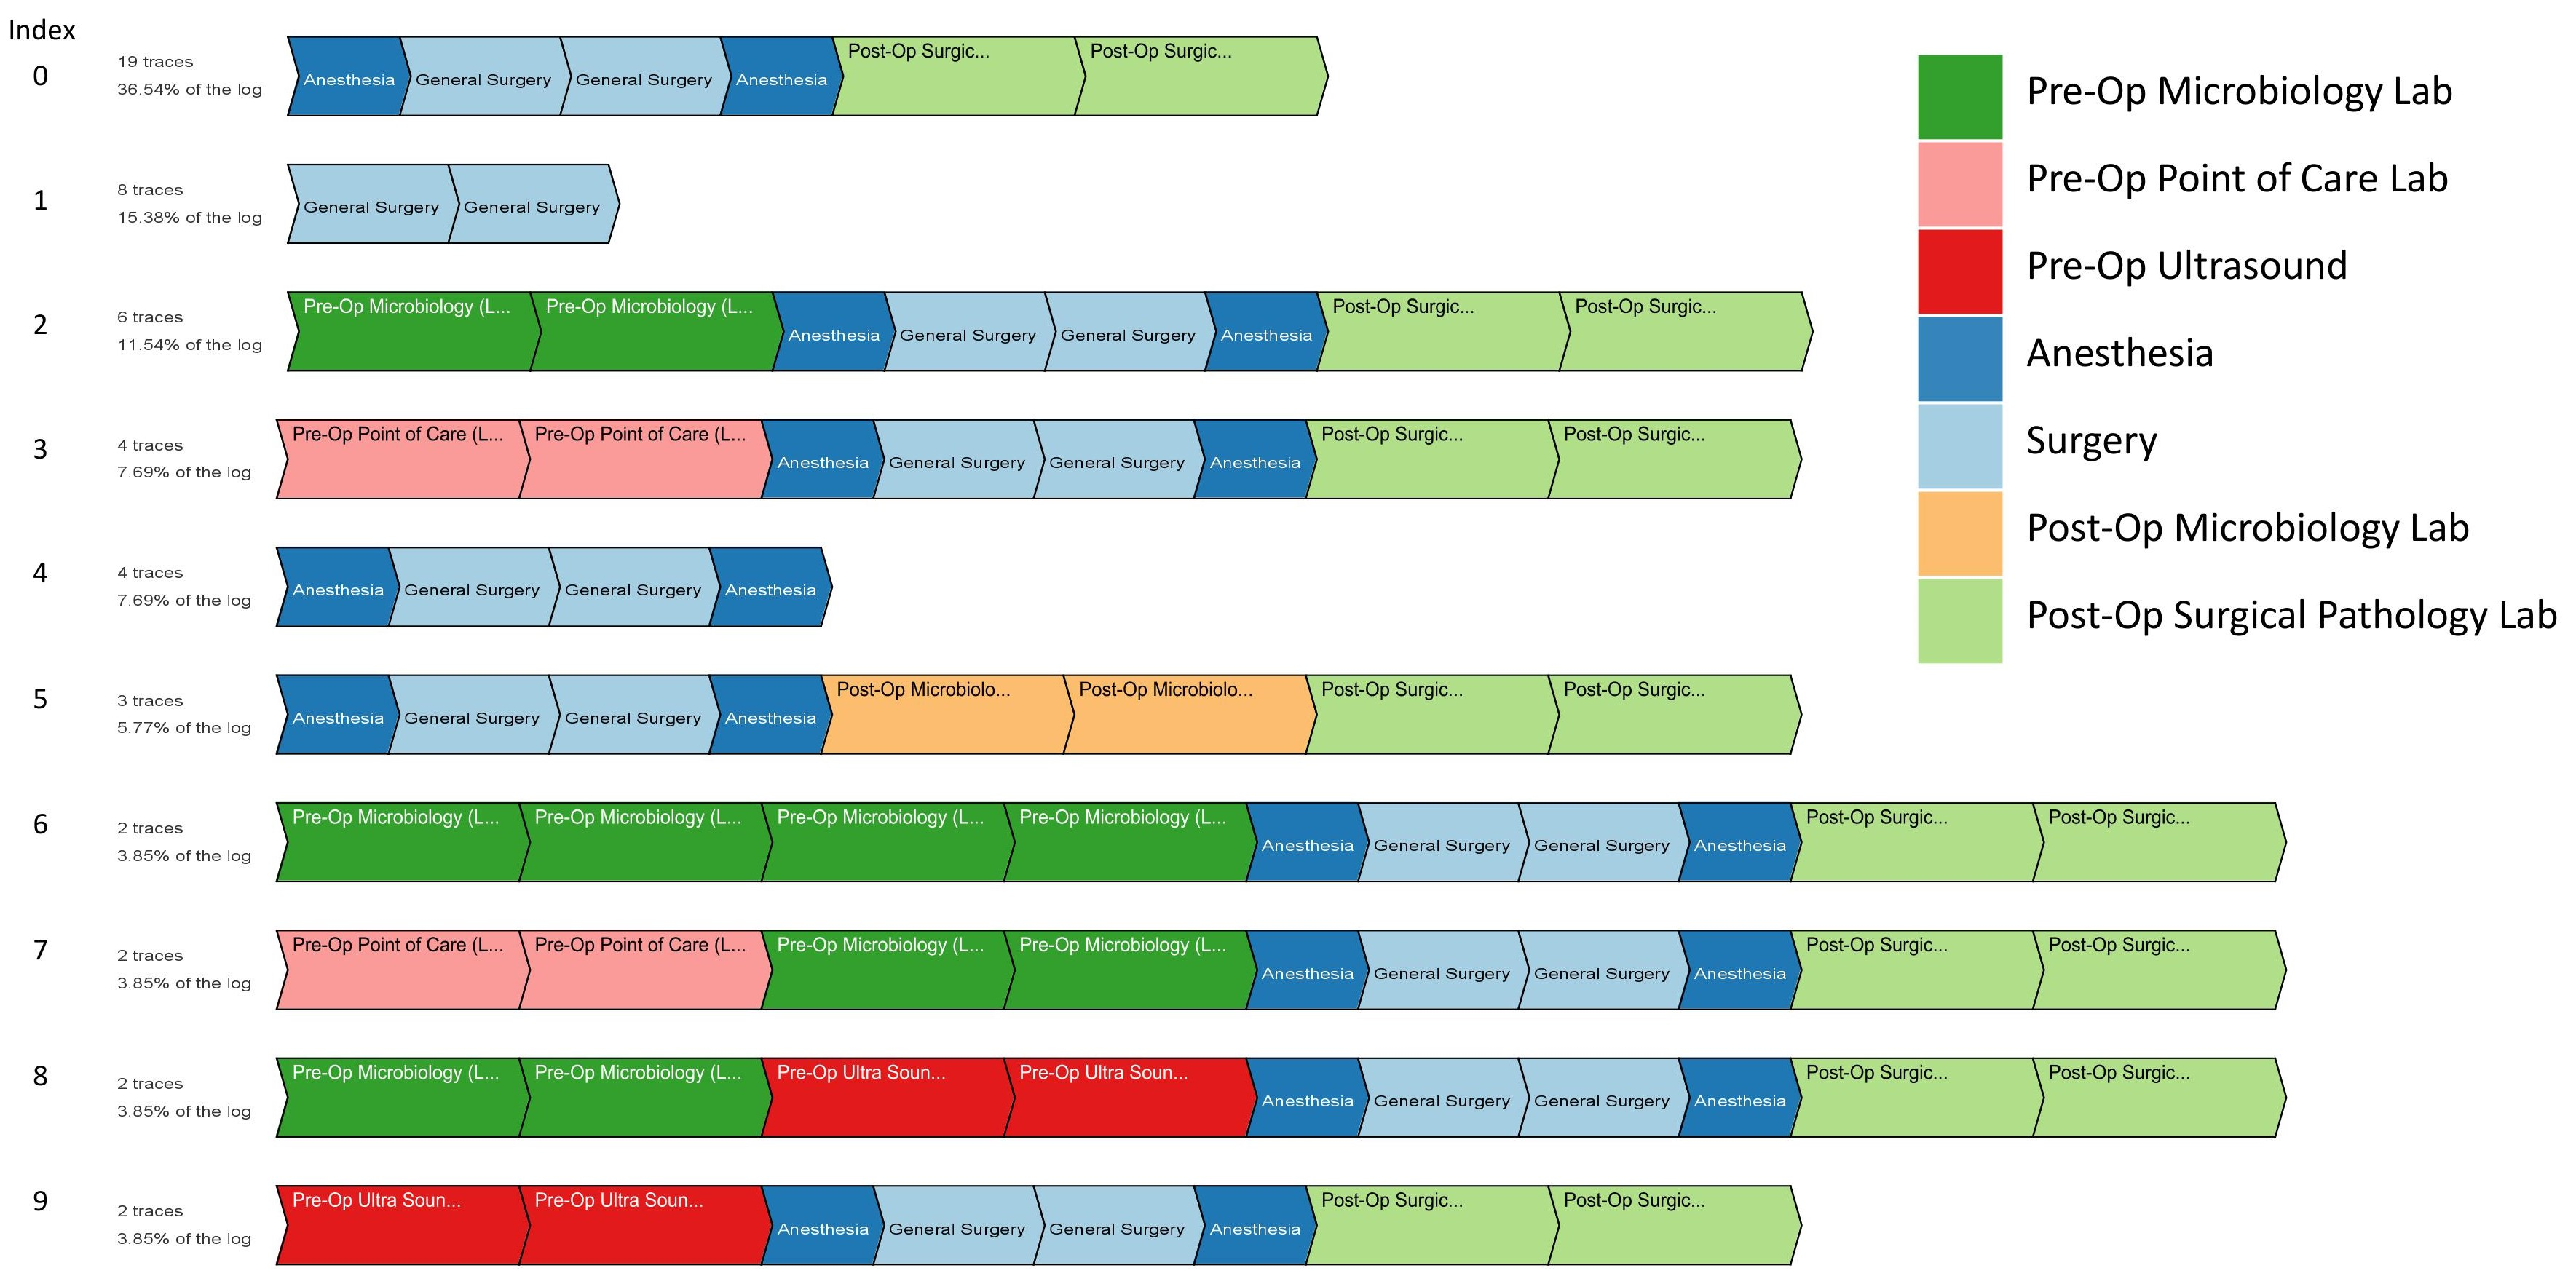
\includegraphics[width=1.5\textwidth]{images/cholecystitis_variant_index_anes.jpg}
\caption{Cholecystitis pathway variant plot auto-generated by ProM's plugin \plugin{Explore Event Log}. For the purpose of readability the legend was added and the statistics on the left are repeated in Tab.~\ref{table:cholecystitis variant table}.
The top three variants account for approximately 63\% of the patient traces.}
\label{fig:cholecystitis pathway variants}
\end{figure}

\begin{table}[t]
\centering
\caption{Statistics of cholecystitis patient traces shown in Fig.~\ref{fig:cholecystitis pathway variants}.}
\label{table:cholecystitis variant table}
\begin{tabular}{llllll}
  \hline
  \hline
Variant &     0  &     1  &     2  &     3  &    4\\
\hline
Patients   &    19 &     8 &     6 &     4 &    4\\
  Percentage &  36.54\% &  15.38\% &  11.54\% &  7.69\% &  7.69\%\\
  \hline
  \hline
Variant &     5  &    6  &    7  &    8 &    9\\
\hline
Patients   &   3 &     2 &     2 &     2 &     2 \\
Percentage &  5.77\% &  3.85\% &  3.85\% &  3.85\% &  3.85\% \\
  \hline
  \hline
\end{tabular}
\end{table}

The cholecystitis pathway model visualized by \texttt{`Inductive Visual Miner'} incorporates activities from the `antibiotics' sub-process and the `monitoring labs' sub-process. A breakdown of the cholecystitis pathway model into one primary pathway and two concurrent sub-processes is shown in Fig.~\ref{fig:cholecystitis pathway model}, and the model notations are summarized in Table \ref{table:notation table}. The first pathway model in Fig.~\ref{fig:cholecystitis pathway model} is the primary pathway, followed by the `antibiotics’ sub-process and the `monitoring labs’ sub-process. Patient traces can execute any combination of the two sub-processes concurrently with the primary pathway. Based on this model, preoperative haematology and chemistry labs tend to span the entire preoperative process, while preoperative antibiotics are taken closer to surgery. The eight patient traces that follow the second pathway variant (index 1) do not conform to this pathway model because of faulty clinical data. These eight patients suffer from both appendicitis and cholecystitis. Appendicitis and cholecystitis are studied as separate healthcare pathways in this study, and activity ‘Anesthesia’ is only recorded in the appendicitis data sets for the eight patients that suffer from both appendicitis and cholecystitis. This demonstrates that conformance analysis is able to detect flaws in the hospital's information system.

\begin{figure}[t]
\centering
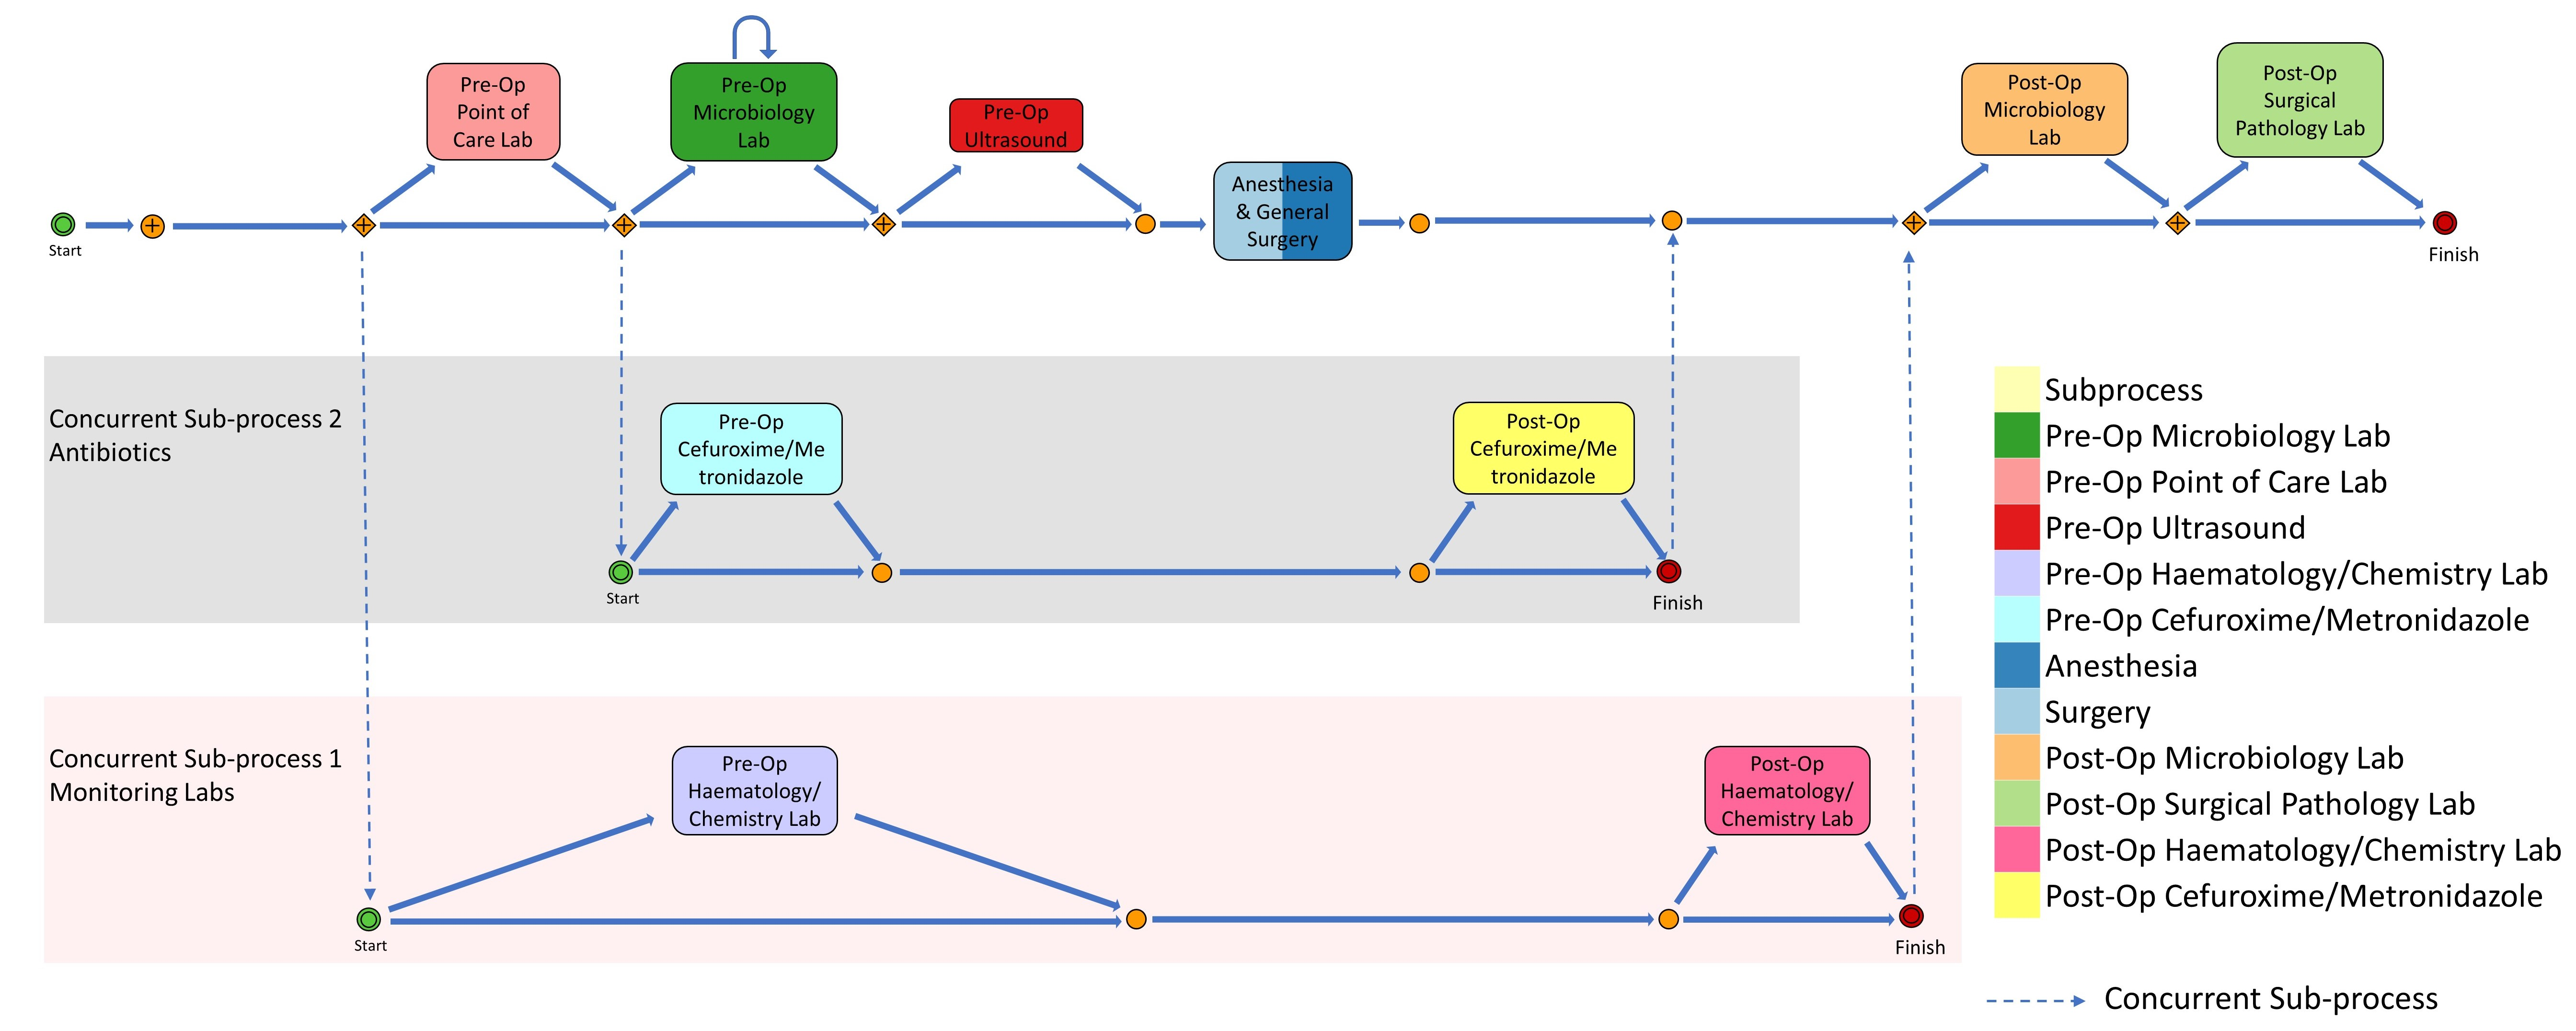
\includegraphics[width=18cm,angle=270]{images/communicative_cholecystitis_process_models_anes.jpg}
\caption{Cholecystitis pathway model using nomenclature of Tab.~\ref{table:notation table}. The model is broken down into one primary pathway and two sub-processes.}
\label{fig:cholecystitis pathway model}
\end{figure}

\subsection{Length of Stays of Cholecystitis Pathway Variants}
Length of stays are analyzed based on the 10 identified cholecystitis pathway variants shown in Fig.~\ref{fig:cholecystitis pathway variants}. Hospital length of stay, measured from admission to discharge, for each of the 10 cholecystitis pathway variants are shown in Fig.~\ref{fig:hospital length of stay cholecystitis}. Postoperative length of stay, measured from leaving theatre to discharge, for each pathway variant is shown in Fig.~\ref{fig:post op length of stay cholecystitis}. Pathway variant 1 appears to have the longest total postoperative length of stay even though it consists of no postoperative activities. All patients that follow pathway variant 1 suffer from both appendicitis and cholecystitis, and the clinicians confirmed that the long total postoperative length of stay could be due to a prolonged recovery time.  

\begin{figure}[t]
\centering
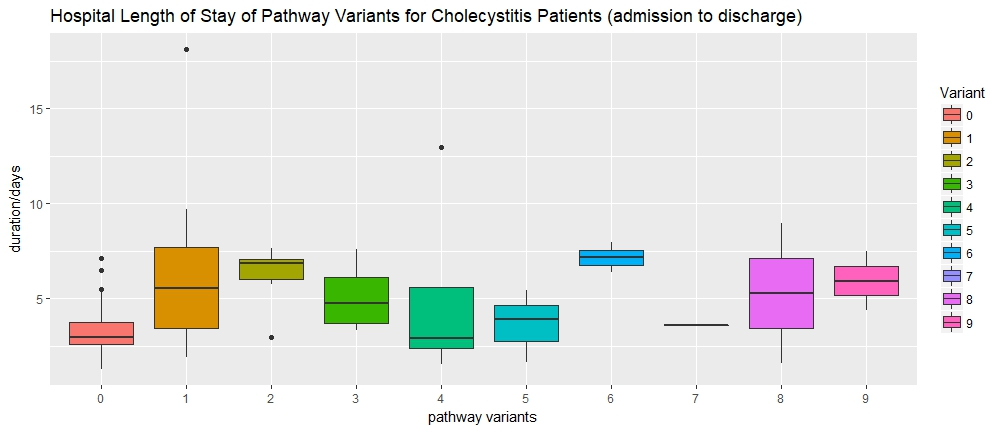
\includegraphics[width=\textwidth]{images/hospital_length_of_stay_cholecystitis_210518.jpeg}
\caption{Hospital length of stay of the 10 cholecystitis pathway variants, measured from admission to discharge.}
\label{fig:hospital length of stay cholecystitis}
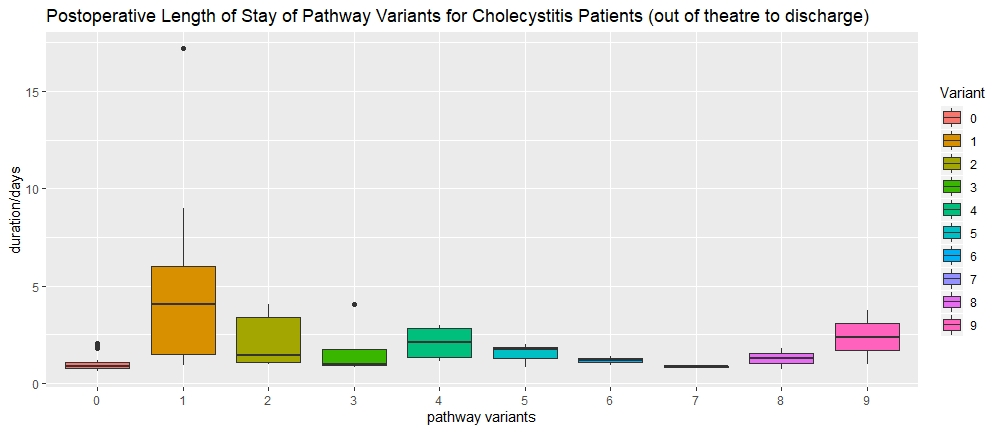
\includegraphics[width=\textwidth]{images/postoperative_length_of_stay_cholecystitis.jpeg}
\caption{Postoperative length of stay of the 10 cholecystitis pathway variants, measured from leaving theatre to discharge.}
\label{fig:post op length of stay cholecystitis}
\end{figure}

\subsection{Probabilistic Machine Learning Model for Postoperative Length of Stay of Appendicitis Patients}
\label{sec:ML}
The following section investigates the question of whether the pathway
variants of the appendicitis case study are relevant features or
covariates for explaining the stochastic volatility of PLS (Fig.~\ref{fig:Geom}a).
This is quite a challenging task, because the individual healing process is expected to depend on personal factors like age \cite{polanczyk2001impact} as well as the individual severity of the appendicitis inflammation, which in general is unknown at this stage of the data analysis, but might be captured by proxies like surgery duration (SD). As mentioned in Sec.~\ref{Sec:DataDescription}, demographics data on cholecystitis patients is unavailable so probabilistic models are only built for appendicitis patients.

\begin{figure}
  \centering
  \begin{tabular}{ll}
    (a) & (b) \\
    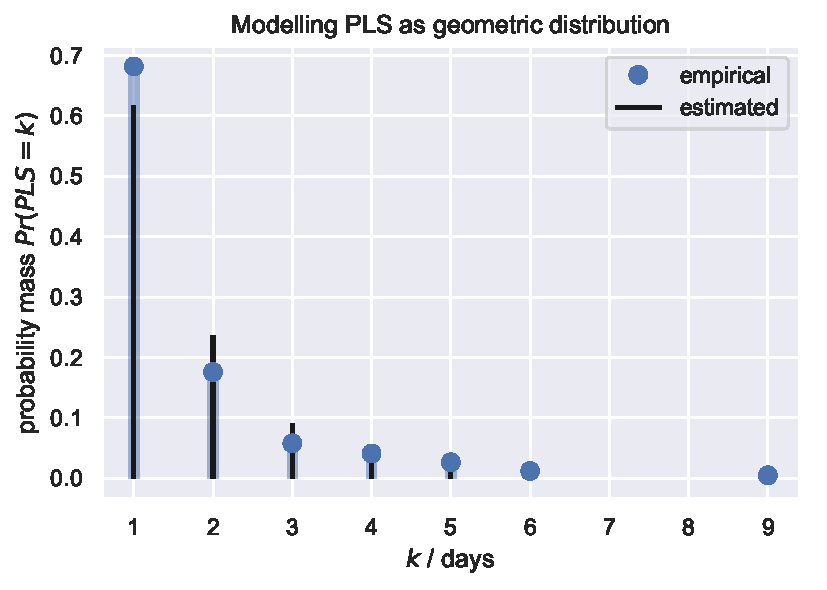
\includegraphics[width=0.5\textwidth]{images/DS19eH1_G0__empirical_geometric.pdf}
    &
    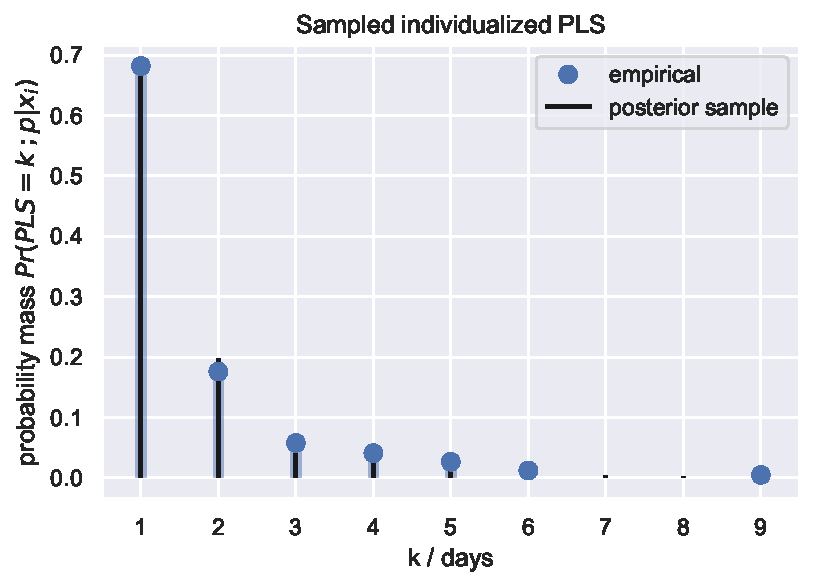
\includegraphics[width=0.5\textwidth]{images/DS19fk1_c0__sampled_posterior.pdf}\\
  \end{tabular}
    \caption{Modelling PLS as geometric distribution without patient
      specific model (a) and with individualised posterior (b) from
      model B (Eq. \eqref{modelB}). Sampling from patient specific
      posterior distributions replicates the observed PLS quite well.
      }
    \label{fig:Geom}
\end{figure}

For the purpose of this analysis, patients' traces with complete
demographic information (415 samples) are selected and
the patients' $PLS$, which is
calculated as the time interval between leaving operating theatre and discharge, is
converted into the number of days after surgery. Therefore, a $PLS$ of
one corresponds to a patient who has been discharged the day after
surgery. Three of the $N=415$  %DS19fA0
patient traces had a PLS of zero, because the surgery ended shortly after midnight and the patients were discharged on the same day. In order to simplify our analysis, the interpretation of PLS was broadened to the number of night rests after surgery, such that the PLS of these three patients could be projected to one.

Analysing the PLS of the 415 appendicitis patients reveals a
histogram which closely resembles a Geometric distribution (Fig.~\ref{fig:Geom}a)
\begin{equation}
Pr(PLS=k) = \text{Geom}(k; p) = (1-p)^{k-1}p^{k},
\end{equation}
parameterized by probability $p$ of being discharged on the $k^\text{th}$ day, respectively $k$ nights of rest after surgery. 
However, estimating $p$ as inverse mean of the observed PLS to 
\begin{equation}
 \hat{p} = \frac{N}{\sum\limits_{i=1}^N PLS_i} \approx 61.8\%	
\end{equation}
reveals that the average discharge probability $\hat{p}$ does not
generalize well over the cohort (Fig.~\ref{fig:Geom}a), because the number of patients being discharged on the first day after surgery is underestimated and the number of patients being discharged on the second and third day after surgery is overestimated.

For the following probabilistic machine learning models, the individualized discharge probability $p_i$ is modelled as a generalized linear model (GLM) using the inverse logistic function (logit) as a link function and the geometric distribution for generating the likelihood. 
For the following analysis, we are comparing two different models of
discharge probability $p_i$ as
\begin{equation}\label{modelA}
  \begin{split}
  \text{logit}(p_i) \sim & \;SD_i + \text{log}(age_i) + 
                            V_{0,i} + V_{1,i} + V_{2,i} + V_{3,i} + V_{0,i}\times\text{log}(age_i) +\\
  &   V_{1,i}\times\text{log}(age_i) + V_{2,i}\times\text{log}(age_i) + V_{3,i}\times\text{log}(age_i),\\
  \end{split}
\end{equation}
which we refer to as \textit{model A}, and
\begin{equation}\label{modelB}
  \begin{split}
  \text{logit}(p_i) \sim & \;SD_i + \text{log}(age_i) +
                                                         V_{0,i} + V_{1,i} + V_{2,i} + V_{3,i} + V_{0,i}\times\text{log}(age_i) +\\
  &    V_{1,i}\times\text{log}(age_i),\\
  \end{split}
\end{equation}
which we refer to as \textit{model B}.
These two models have been selected because they were the most
credible based on the widely applicable information criterion
(WAIC) and leave-one-out cross-validation (LOO) statistics
\cite{Vehtari2017_WAIC_LOO}.
The explanatory variables $V_{j,i}$ are categorical with 
\begin{equation}
V_{j,i} = \begin{cases}
	1: & V_{j,i} = j,\\
        0: & \text{otherwise}.
\end{cases}
\end{equation}
Therefore, the case $V_{0,i}=V_{1,i}=V_{2,i}=V_{3,i}=0$ corresponds to variants V4--V12 of Fig.~\ref{fig:appendicitis pathway variants}.
Models A and B make the simplifying assumption that the individualised
probability of discharge $Pr(PLS_i=k|x_i)$ can be estimated from 
\begin{equation}
x_i = (SD_i, \text{log}(age_i), V_{0,i}, V_{1, i}, V_{2, i}, V_{3, i}).
\end{equation}
 being available at the end of surgery, when future treatment steps and therefore the complete pathway variant for the respective $i^\text{th}$ patient have been decided on:
\begin{equation}
\begin{split}
Pr(PLS_i=k|x_i) & = \text{Geom}\left(k;p(x_i)\right) \\
& = \left(1-p(x_i)\right)^{k-1}\left(p(x_i)\right)^{k} \\
%& = \left(1-\mathbb{E}_{x_i}[p]\right)^{k-1}\left(\mathbb{E}_{x_i}[p]\right)^{k} \\
          %        & = \left(1-\text{logistic}(f(x_i))\right)^{k-1}\text{logistic}(f(x_i))^{k} \\
          %        & = \left(1+e^{f(x_i)}\right) \left(2 + e^{-f(x_i)} + e^{f(x_i)}\right)^{-k}
\end{split}
\end{equation}
with $p(x_i)$ being modelled either by Eq. \eqref{modelA} or
\eqref{modelB}.
    
The statistical model has been fitted using PyMC3
\citep{Salvatier2016_PyMC3} version 0.24.2 using the No-U-Turn Sampler
(NUTS) with 20,000 samples, 2,000 tuning steps, 2 chains, and an
acceptance rate of 90\%. The 95\% credible intervals of the estimated
model coefficients are shown in Fig.~\ref{fig:forest_plots}. The
Gelman-Rubin convergence statistic Rhat is close to one for all
coefficients (Tab.~\ref{tab:coeff}). 
However, for Model A the coefficients of the interaction terms
$\text{log}(age_i)\times V_2$ and $\text{log}(age_i)\times V_3$ are
close to zero with negative expectation values but a 25\% and 15\%
probability of being larger than zero (Tab.~\ref{tab:coeff}). 
Therefore, we have decided to focus the following analysis of the
fitted model on Eq.~\eqref{modelB} for which all credible intervals
exclude zero (Fig.~\ref{fig:forest_plots}b).
However, this does not change the overall trend depicted in Fig.~\ref{fig:posterior}.
It is important to note that both the coefficients of $SD$ and $\text{log}(age)$ are negative. This means that for the base model of variants V4--V12 as well as variants V2 and V3, the probability of discharge decreases with increasing SD and age. 
Compared to the base model, Variants V2 and V3 have a higher discharge probability because both coefficients are positive. 
The situation is more complicated for variants V0 and V1, because their coefficients are negative but the coefficients of their interaction terms with $\text{log}(age)$ are positive, which basically counterbalances the effect of $\text{log}(age)$.

\begin{figure}
  \centering
    \begin{tabular}{ll}
(a) Model A \eqref{modelA} & (b) Model B \eqref{modelB}\\
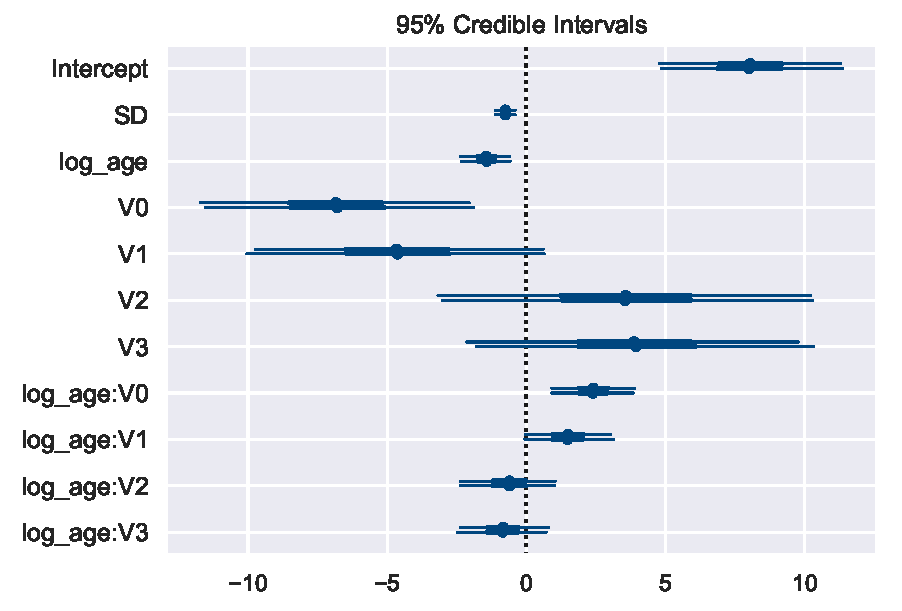
\includegraphics[width=0.5\textwidth]{images/DS19fm0_c0__forestplot_model_A.pdf}&
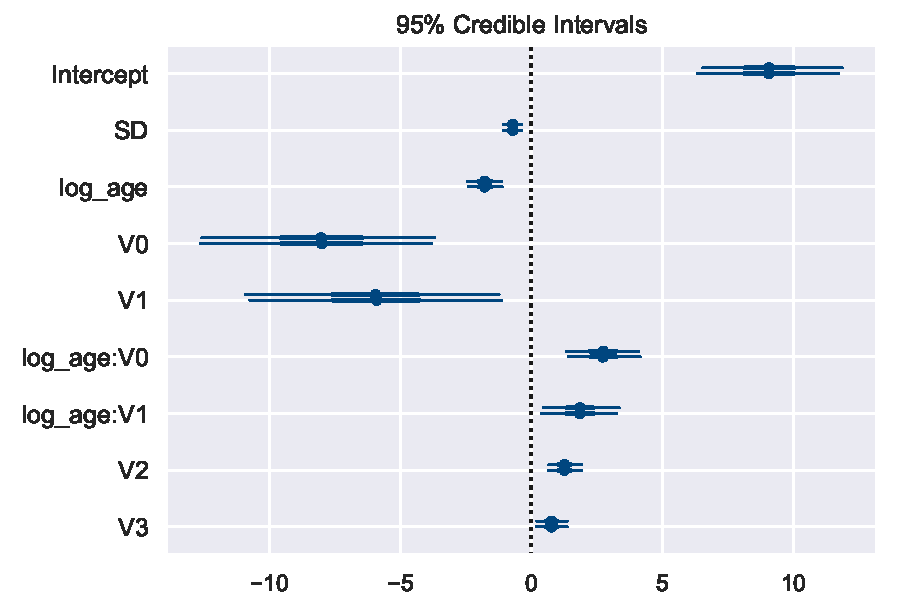
\includegraphics[width=0.5\textwidth]{images/DS19fk1_c0__forestplot_model_B}\\
\end{tabular}
    \caption{Credible intervals for models A \eqref{modelA} and B \eqref{modelB}.}
    \label{fig:forest_plots}
\end{figure}

\begin{table}
\caption{\label{tab:coeff} Coefficients of model B. Rhat is the
  potential scale reduction factor. A value of one indicates
  convergence.}
\centering
\begin{tabular}{lrrrr}
\hline
\hline
{} &      mean &    hpd\_2.5 &   hpd\_97.5 &      Rhat \\
\hline
Intercept  &  9.09 &   6.48 &  11.85 &  0.999988 \\
SD        & -0.71 &  -1.059 &  -0.371 &  0.999987 \\
log\_age    & -1.781 &  -2.46 &  -1.154 &  0.999988 \\
V0         & -8.04 & -12.56 &  -3.70 &  0.999980 \\
V1         & -5.95 & -10.82 &  -1.186 &  1.000013 \\
log\_age:V0 &  2.75 &   1.365 &   4.12 &  0.999980 \\
log\_age:V1 &  1.864 &   0.423 &   3.32 &  1.000013 \\
V2         &  1.267 &   0.646 &   1.901 &  1.000062 \\
V3         &  0.766 &   0.199 &   1.363 &  1.000046 \\
\hline
\hline
\end{tabular}
\end{table}


\begin{figure}
    \centering
    \begin{tabular}{ll}
(a)  & (b) \\
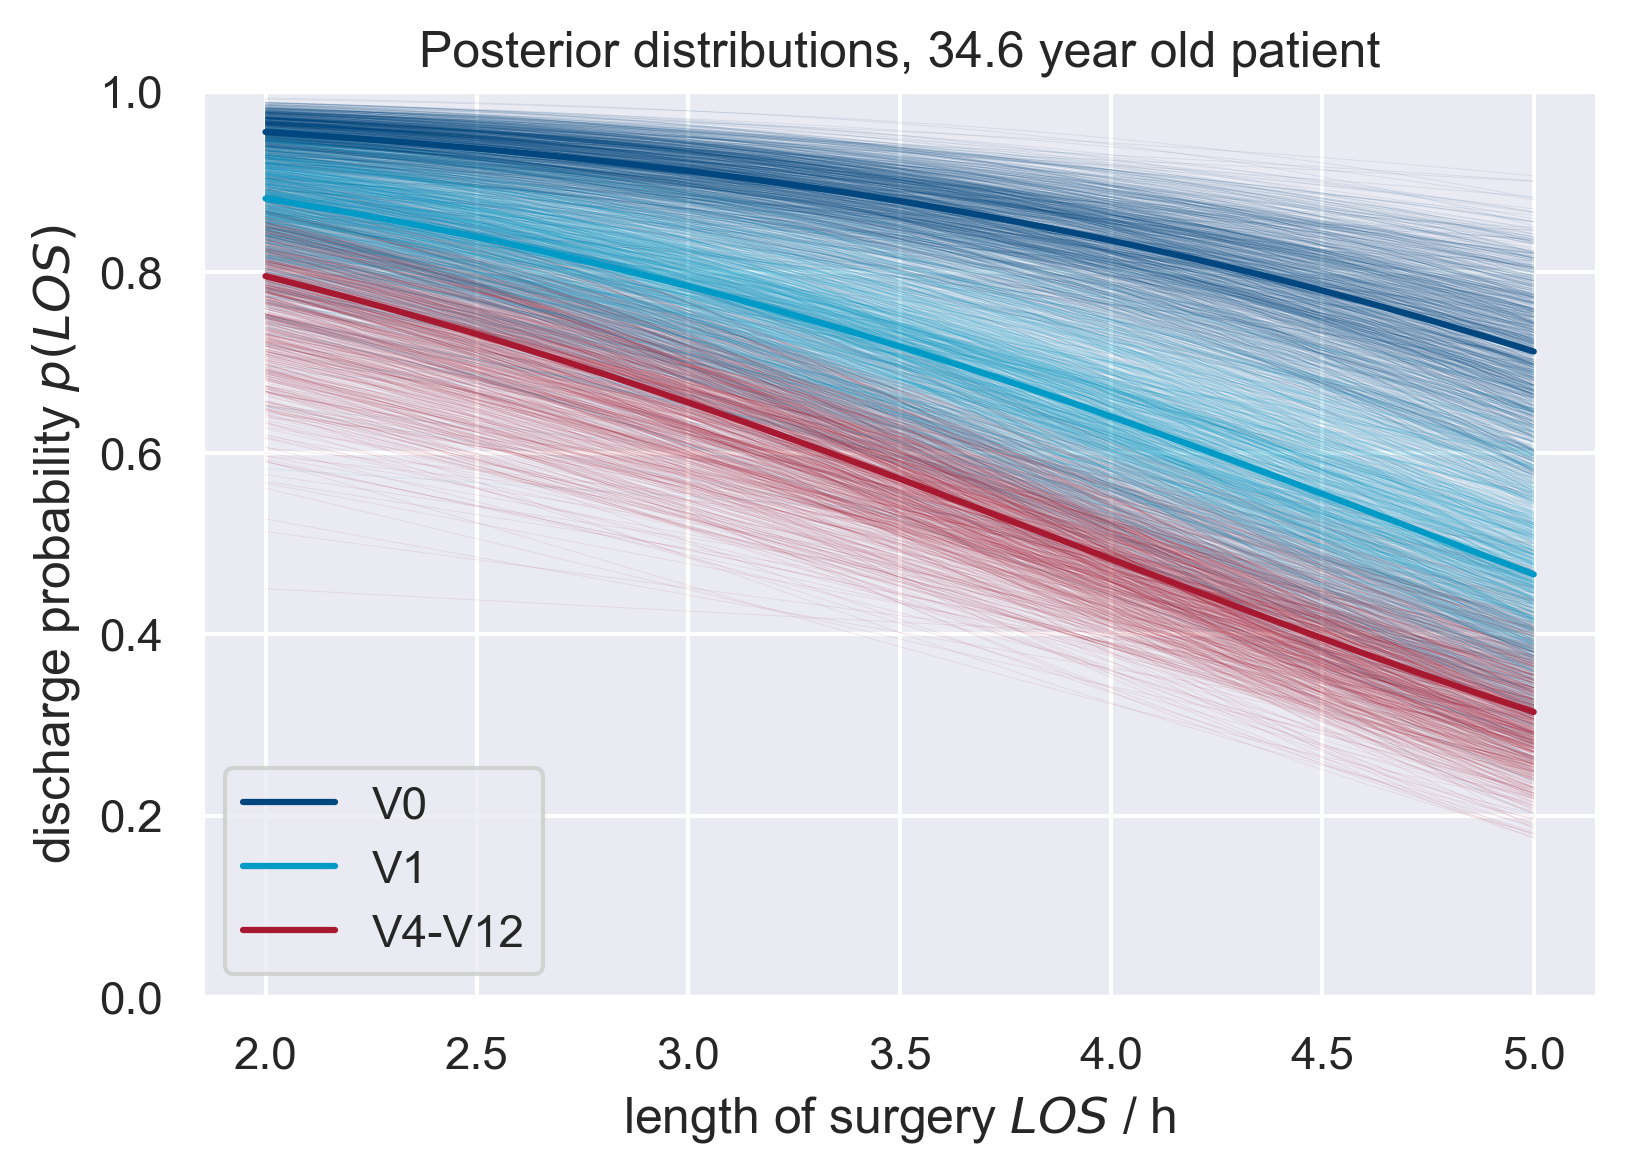
\includegraphics[width=0.5\textwidth]{images/DS19fk1_c0__p_LoS__model_B__traces_V0_V4-12__age_mean.png}&
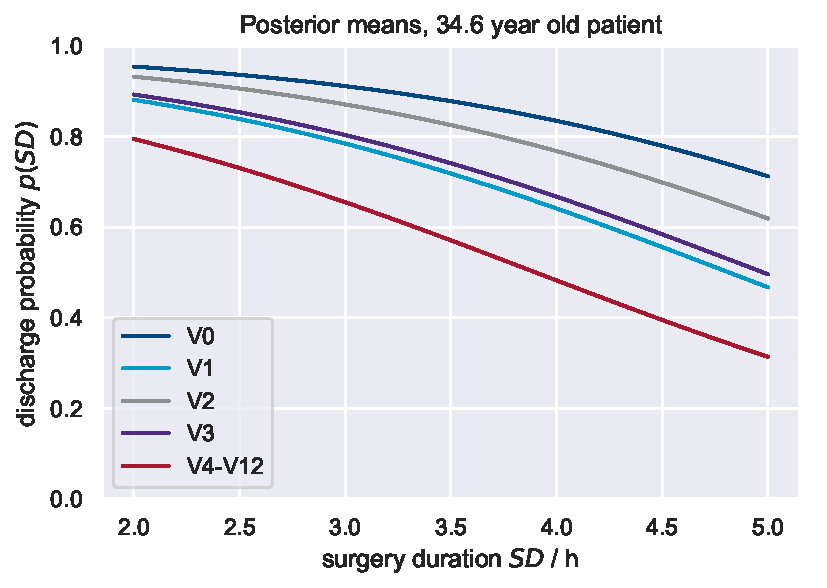
\includegraphics[width=0.5\textwidth]{images/DS19fk1_c0__p_LoS__model_B__mean__age_mean.pdf}\\
(c) & (d) \\
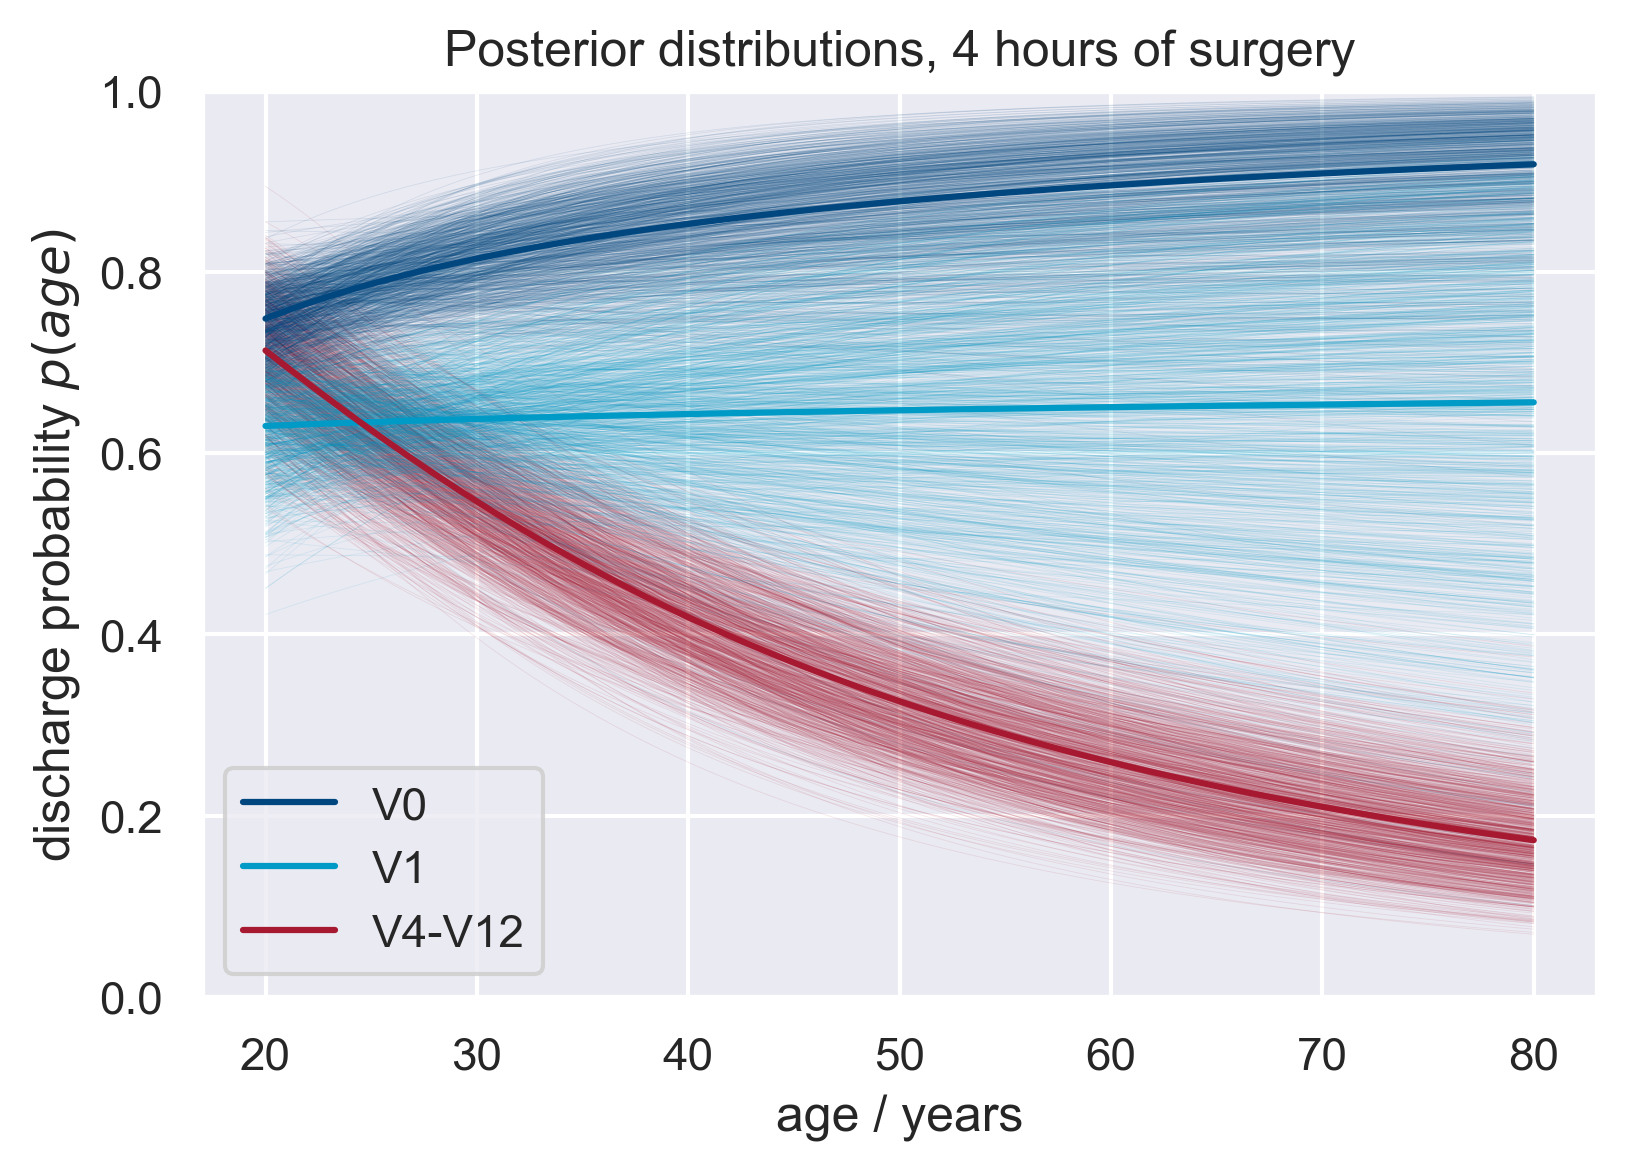
\includegraphics[width=0.5\textwidth]{images/DS19fk1_c0__p_age__model_B__traces__LoS_4h.png}&
\includegraphics[width=0.5\textwidth]{images/DS19fk1_c0__p_age__model_B__mean__LoS_4h.pdf}\\
\end{tabular}
    \caption{Posterior distributions and corresponding means for
      different pathway variants of model B \eqref{modelB}. Trends with respect to
      SD and age are similar for model A \eqref{modelB}.}
    \label{fig:posterior}
\end{figure}

This is visualized in Fig.~\ref{fig:posterior}, which shows the posterior distributions of discharge probability $p_i$ as function of SD (Fig.~\ref{fig:posterior}(a)) and age (Fig.~\ref{fig:posterior}(c)). While the discharge probability decreases with increasing SD for all pathway variants (Fig.~\ref{fig:posterior}(b)), the effect is different for age. 
The discharge probability $p_i$ decreases for Variants V2, V3, and V4-V12 with increasing age of the patients, while its expectation value is constant for $V1$ and even increases by nearly 10\% for V0. Note, that the corresponding graphics for model A \eqref{modelA}, which are not shown here, resemble nearly the same correlations. 
From the clinical perspective, the difference in effects of age with
respect to the pathway variants might be related to the fact that the
most common pathway variants V0 and V1 are predominantly followed by younger patients (Fig.~\ref{Fig:boxplot}) and possibly older patients, for whom no complications are expected. 
However, the uncertainty of discharge probabilities for V1 is significantly larger compared to V0.

\begin{figure}
  \centering
  \includegraphics[width=0.618\textwidth]{images/DS19fA0_Lin20180730a__boxplot_age_variant.pdf}
\caption{Boxplot of patients' age for pathway variants of the
  appendicitis model.}
\label{Fig:boxplot}
\end{figure}
%\subsection{Cholecystitis Pathway Variants}
This section shows the cholecystitis pathway variant plot auto-generated by ProM. Cholecystitis pathway variants are analyzed without activities from the `antibiotics' sub-process and the `monitoring labs' sub-process (see section 3.7 for the activities from the two sub-processes). Clinicians confirmed that these sub-processes are standard monitoring and maintenance systems while the patient is waiting for further diagnosis. Only analyzing activities from the primary cholecystitis pathway significantly reduces the level of clinical variation between patient traces.

The cholecystitis pathway model consists of 10 pathway variants. The 10 pathway variants from the cholecystitis pathway model are shown in Fig.~\ref{fig:cholecystitis pathway variants}, and the number of patient traces that follow each pathway variant are listed in Table \ref{table:cholecystitis variant table}. Pathway variants from Fig.~\ref{fig:cholecystitis pathway variants} are ordered from the most frequent (index 0) to the least frequent (index 9). The most frequent pathway variant (index 0) consists of anesthesia, surgery, and surgical pathology lab. The second pathway variant (index 1) includes surgery without anesthesia because of faulty clinical data.

\begin{figure}[t]
\hspace{-2cm}
\includegraphics[width=1.5\textwidth]{images/cholecystitis_variant_index_anes.jpg}
\caption{Cholecystitis pathway variants auto-generated by ProM and appended with a legend. The top three pathway variants account for approximately 63\% of the patient traces. The statistics on the left are not readable in this reproduction but are listed in Table \ref{table:cholecystitis variant table}.}
\label{fig:cholecystitis pathway variants}
\end{figure}

\begin{table}[t]
\centering
\caption{Number of patient traces that follow each cholecystitis pathway variant.}
\label{table:cholecystitis variant table}
\begin{tabular}{ l l l }
 \hline
 Index & Number of Patient Traces & Percentage of Patients \% \\ 
 \hline
 0 & 19 & 36.54\\ 
 \hline
 1 & 8 & 15.38\\ 
 \hline
 2 & 6 & 11.54\\ 
 \hline
 3 & 4 & 7.69\\ 
 \hline
 4 & 4 & 7.69\\ 
 \hline
 5 & 3 & 5.77\\ 
 \hline
 6 & 2 & 3.85\\ 
 \hline
 7 & 2 & 3.85\\ 
 \hline
 8 & 2 & 3.85\\ 
 \hline
 9 & 2 & 3.85\\ 
 \hline
\end{tabular}
\end{table}

\subsection{Cholecystitis Pathway Model}
The cholecystitis pathway model visualized by \texttt{`Inductive Visual Miner'} incorporates activities from the `antibiotics' sub-process and the `monitoring labs' sub-process. A breakdown of the reformulated cholecystitis pathway model into one primary pathway and two concurrent sub-processes is shown in Fig.~\ref{fig:cholecystitis pathway model}, and the model notations are summarized in Table \ref{table:notation table}. The first pathway model in Fig.~\ref{fig:cholecystitis pathway model} is the primary pathway, followed by the `antibiotics’ sub-process and the `monitoring labs’ sub-process. Patient traces can execute any combination of the two sub-processes concurrently with the primary pathway. The eight patient traces that follow the second pathway variant (index 1) do not conform to this pathway model because of faulty clinical data. Based on this model, pre-operation haematology and chemistry labs tend to span the entire pre-operation process, while pre-operation antibiotics are taken closer to surgery.

\begin{figure}[t]
\centering
\includegraphics[width=18cm,angle=270]{images/communicative_cholecystitis_process_models_anes.jpg}
\caption{Cholecystitis pathway model. The model is broken down into one primary pathway and two sub-processes.}
\label{fig:cholecystitis pathway model}
\end{figure}

\section{Discussion from Thesis}
The aim of this study is to use business process modelling methods to design a process mining pipeline that supports discovery, conformance analysis, and enrichment of healthcare pathways from hospital health records, and to apply the designed pipeline to two clinical case studies. Results from the two case studies indicate that the designed pipeline with ProM as the main process mining tool is effective for mining both simple and complex healthcare pathway models to produce a concise form that is easy for clinical interpretation. This chapter discusses the advantages and limitations of the proposed healthcare pathway mining method for the three stages of analysis (i.e. healthcare pathway discovery, conformance, and enrichment). Future research directions that would maximize this study’s potential for industrial implementation are also discussed.

The discovery stage of the designed process mining pipeline provides an unbiased view of real patient experiences through the treatment process. The proposed approach to pathway discovery is data-based, so the accuracy of the output healthcare pathway model is highly dependent on data accuracy. Incorrectly logged health records in hospital information systems can lead to an inaccurate representation of real patient experiences through the treatment process, so clinicians must be consulted to determine if unexpected results are caused by faulty data. The main advantage of the proposed approach is that healthcare pathway visualization is automatic, and this means that the healthcare pathway mining pipeline has the potential to be fully automated in the future. Health records from the same hospital usually follow systematic formats and notations, so the process of converting electronic health records to clinical event logs compatible with business process mining software can be automated. The main challenge to automating the entire healthcare pathway discovery process is the event log processing steps required to reduce clinical variations. Even though the chapter on healthcare pathway mining methodology (Chapter 2) provides guidelines on processing steps that are effective for reducing unnecessary clinical variations in event logs, a certain level of clinical input is still required to ensure that no crucial information is filtered. In the first case study (see Chapter 3), appendicitis and cholecystitis pathways both contain repetitive activity patterns (i.e. antibiotics and monitoring labs) that result in incomprehensible spaghetti-models, and these patterns are identified by manual inspection of the pathway variants. There is potential for the process mining pipeline proposed in this study to be combined with clinical pattern mining algorithms developed in previous studies (e.g. the SCP-Miner and CCP-Miner developed by Huang, Lu, and Duan [16]) so that repetitive activity patterns can be identified and condensed automatically. Further research is required to determine the compatibility of the proposed process mining pipeline with various pattern mining algorithms.

The appendicitis and cholecystitis pathway models, from the first clinical case study, and the ambulatory cardiac care pathway model, from the second clinical case study, are all confirmed by clinicians to be easy to interpret and clinically meaningful, but one major limitation of the proposed pathway discovery approach is that the discovered healthcare pathway models can contain pathways that are not executed by any patient traces in the clinical event log. This is because the process mining software arranges all activities into a coherent pathway model by a configuration that summarizes all pathway variants, but a configuration that summarizes pathway variants does not guarantee that all pathways in the final healthcare pathway model make sense clinically. This also means that the pathway representation of models discovered by the proposed pipeline is unable to accurately capture all relations between activities. For example, the ambulatory cardiac care pathway model from the second case study (see Figure 56) shows that it is possible for patients to perform activity ‘Coronary Angiogram’ without performing ‘First Cardiology’ first. Close inspection of the event log revealed that patients who perform ‘Coronary Angiogram’ always perform ‘First Cardiology’ first, but this relation between the two activities is not evident in the discovered pathway model. Analysis of pathway variants instead of the pathway model does portray the true relations between all activities but this is not a realistic approach for complex healthcare pathways. For relatively simple healthcare pathways like the appendicitis and cholecystitis case study, patient traces can be organized into a manageable number of unique pathway variants and all variants can be analyzed individually. For complex healthcare pathways like the ambulatory cardiac care case study, patient traces cannot be organized into a manageable number of pathway variants because the level of variation between patients is too high. The healthcare pathway discovery stage of the methods presented here provides a concise overview of the fundamental structure of the overall pathway but does not always effectively capture the true relations between clinical activities. 
The conformance analysis stage of the designed process mining pipeline effectively identifies and visualizes patient deviations from the discovered healthcare pathway models. Even though this study only analyzes patient conformance to the discovered healthcare pathways, the same method could be applied analyze patient conformance to predefined ideal pathways or new pathway designs. The proposed approach to conformance analysis could be extended in the future to a monitoring tool to maintain quality of care for all patients. It is very difficult for clinicians to manually track individual patient traces through the treatment process and ensure that they are conforming to standard protocols. Identifying unwarranted deviations and making the required interventions early in the process has the potential to improve health outcomes and decrease cost. Even though the proposed approach effectively visualizes patient deviations, it cannot distinguish between clinically significant deviations and minor deviations that have no influence on patient health outcome. For example, some deviations are the results of scheduling availability and the order in which a required set of clinical activities are executed is not always relevant to health outcome. The proposed conformance analysis approach cannot automatically identify clinically significant deviations, and reasons for all deviations must be investigated manually. This is a major obstacle to future hospital implementation of the proposed pipeline, because it is inefficient and impractical to alert clinicians to minor patient deviations. Further research is required to develop a more specialized tool for conformance analysis that is able to classify patient deviations according to their association with patient health outcome.

The enrichment stage of the designed process mining pipeline is effective for identification of bottlenecks and treatment delays in healthcare pathways. The enrichment stage of the ambulatory cardiac care case study revealed that waiting times for transthoracic echo are exceedingly long (see §4.7), and resource reallocation is recommended to reduce the treatment delay. The effects of the delay on patient health outcome can be further investigated by computer simulations, but more clinical data is required for this approach. Analysis of waiting times and hospital length of stays is based on the assumption that the occurring timestamps of clinical activities are accurate. North Shore Hospital has an automated information system that stores patient records in real time and accuracy of the timestamps in the two case studies is therefore high, but the precision of activity timestamps is not always consistent across hospital systems. For example, one clinical department could record the exact time of day an activity is executed, while another department only records the date of execution. This leads to a margin of error of 24 hours, and this margin of error must be taken into account when interpreting the results. Accuracy and precision of clinical data must be assessed when the proposed pipeline is applied to new clinical case studies.

Analysis of pathway performance based on pathway variants reveals associations between clinical activities and performance indicators, but associations do not necessarily indicate causation. For example, the appendicitis pathway variants from the first case study that consist of postoperative imaging activities generally have longer postoperative length of stays, even though larger samples are required to confirm this connection (see §3.9). One possible explanation is that appendicitis patients that develop extra complications are more likely to require postoperative imaging activities. These are also the patients that remain under monitoring for a longer time period and hence have a delayed discharge date. Similarly, the ambulatory cardiac care pathway variants from the second case study that consist of visits to the emergency department generally have higher mortality rates (see §4.84.8). In both of these cases, patient condition is the main factor that influences the pathway performance indicators.
Dr. Andreas W. Kempa-Liehr’s work on developing probabilistic models to predict postoperative length of stay using information from the discovered healthcare pathway has the potential to improve the efficiency of hospital scheduling and resource allocation. This also shows that the proposed process mining pipeline has the potential to support the development of machine learning models for the prediction of performance indicators. A future improvement that could be made to the proposed pipeline is the incorporation of clinical diagnosis into the healthcare pathway models. Incorporating clinical diagnosis into pathway models allows for the identification of critical decision points where pathway variants diverge, but the main challenge is obtaining access to clinical diagnostic data. Overall, there is potential for the use of business process modelling techniques to improve the method of analysis of healthcare pathways, but the capability of other more specialized business process mining software should also be explored.

\section{Conclusion}
Healthcare pathways are critical for maintaining quality of care and
improving health outcome for all patients, but there is no consensus
on a healthcare pathway mining pipeline suitable for hospital
implementation that supports pathway discovery from hospital health
records.
Business process modelling methods are used to design a process mining
pipeline that produces concise and comprehensible healthcare pathway
models from hospital records, and supports conformance analysis and
enrichment of the discovered pathways.
The proposed process mining pipeline successfully constructs concise
pathway models for the appendicitis and cholecystitis case studies.
The produced healthcare pathway models are easy for clinical
interpretation and provide an unbiased overview of real patient traces
through the treatment process.
Probabilistic machine learning models for predicting postoperative
length of stay, using information extracted by the process mining
pipeline, is showing promising results.
This means that the proposed mining pipeline has the potential to
support the development of machine learning models to further relate
healthcare pathways to performance indicators.
This study has established the use of business process modelling methods for the improvement of healthcare pathway mining methods, and there is value in investigating the capabilities of other business process modelling tools for healthcare pathway mining purposes.

\begin{table}[h]
\centering
\begin{tabular}{p{11cm}} 
 Summary points\\ 
 What was already known:
 \begin{itemize}
     \item Healthcare pathways are critical for reducing clinical variability, affecting operational excellence, and thereby maximizing health outcomes.
     \item  Most healthcare pathways result from clinician-led practice rather than explicit pathway design via a consensus model and systems approach. 
     \item  There is currently no consensus on a systematic healthcare pathway mining method that supports explicit design and conformance analysis of concise and comprehensible healthcare pathway models.
 \end{itemize}
 What this study adds:
 \begin{itemize}
     \item  The use of business process modelling methods improves the automatic mapping of healthcare pathways from clinical data.
     \item The application of business process modelling methods to
       healthcare pathway enables deviations from typical treatment
       pathways to be identified, all using standard clinical data
       timestamps.
     \item Probabilistic machine learning models enable the prediction
       of patient specific discharge probabilities, which lead to
       patient specific postoperative
       length of stay distributions.
 \end{itemize}
\end{tabular}
\end{table}


\section*{Author Contributions}
All authors have made substantial contribution to this study and approved the final manuscript.

\section*{Acknowledgements}
This research has been funded by the Precision Driven Health research partnership (project number 1209).

\section*{Declaration of Competing Interests}
The authors declare that they have no competing interests for this study.

\bibliography{mybibfile}

\begin{appendix}
\subsection{Cholecystitis Pathway Variants}
This section shows the cholecystitis pathway variant plot auto-generated by ProM. Cholecystitis pathway variants are analyzed without activities from the `antibiotics' sub-process and the `monitoring labs' sub-process (see section 3.7 for the activities from the two sub-processes). Clinicians confirmed that these sub-processes are standard monitoring and maintenance systems while the patient is waiting for further diagnosis. Only analyzing activities from the primary cholecystitis pathway significantly reduces the level of clinical variation between patient traces.

The cholecystitis pathway model consists of 10 pathway variants. The 10 pathway variants from the cholecystitis pathway model are shown in Fig.~\ref{fig:cholecystitis pathway variants}, and the number of patient traces that follow each pathway variant are listed in Table \ref{table:cholecystitis variant table}. Pathway variants from Fig.~\ref{fig:cholecystitis pathway variants} are ordered from the most frequent (index 0) to the least frequent (index 9). The most frequent pathway variant (index 0) consists of anesthesia, surgery, and surgical pathology lab. The second pathway variant (index 1) includes surgery without anesthesia because of faulty clinical data.

\begin{figure}[t]
\hspace{-2cm}
\includegraphics[width=1.5\textwidth]{images/cholecystitis_variant_index_anes.jpg}
\caption{Cholecystitis pathway variants auto-generated by ProM and appended with a legend. The top three pathway variants account for approximately 63\% of the patient traces. The statistics on the left are not readable in this reproduction but are listed in Table \ref{table:cholecystitis variant table}.}
\label{fig:cholecystitis pathway variants}
\end{figure}

\begin{table}[t]
\centering
\caption{Number of patient traces that follow each cholecystitis pathway variant.}
\label{table:cholecystitis variant table}
\begin{tabular}{ l l l }
 \hline
 Index & Number of Patient Traces & Percentage of Patients \% \\ 
 \hline
 0 & 19 & 36.54\\ 
 \hline
 1 & 8 & 15.38\\ 
 \hline
 2 & 6 & 11.54\\ 
 \hline
 3 & 4 & 7.69\\ 
 \hline
 4 & 4 & 7.69\\ 
 \hline
 5 & 3 & 5.77\\ 
 \hline
 6 & 2 & 3.85\\ 
 \hline
 7 & 2 & 3.85\\ 
 \hline
 8 & 2 & 3.85\\ 
 \hline
 9 & 2 & 3.85\\ 
 \hline
\end{tabular}
\end{table}

\subsection{Cholecystitis Pathway Model}
The cholecystitis pathway model visualized by \texttt{`Inductive Visual Miner'} incorporates activities from the `antibiotics' sub-process and the `monitoring labs' sub-process. A breakdown of the reformulated cholecystitis pathway model into one primary pathway and two concurrent sub-processes is shown in Fig.~\ref{fig:cholecystitis pathway model}, and the model notations are summarized in Table \ref{table:notation table}. The first pathway model in Fig.~\ref{fig:cholecystitis pathway model} is the primary pathway, followed by the `antibiotics’ sub-process and the `monitoring labs’ sub-process. Patient traces can execute any combination of the two sub-processes concurrently with the primary pathway. The eight patient traces that follow the second pathway variant (index 1) do not conform to this pathway model because of faulty clinical data. Based on this model, pre-operation haematology and chemistry labs tend to span the entire pre-operation process, while pre-operation antibiotics are taken closer to surgery.

\begin{figure}[t]
\centering
\includegraphics[width=18cm,angle=270]{images/communicative_cholecystitis_process_models_anes.jpg}
\caption{Cholecystitis pathway model. The model is broken down into one primary pathway and two sub-processes.}
\label{fig:cholecystitis pathway model}
\end{figure}
\end{appendix}
\end{document}

\end{document}